\documentclass[11pt,a4paper]{article}

%------------------------------------------------
% Packages and formatting
%------------------------------------------------
%================================================
% Page layout
%================================================

\usepackage[
    a4paper,
    margin=2.5cm
]{geometry}

%================================================
% Mathematics
%================================================

\usepackage{amsmath}
\usepackage{amssymb}
\usepackage{amsfonts}
\usepackage{bm}

%================================================
% Figures and tables
%================================================

\usepackage{graphicx}
\usepackage{float}
\usepackage{subcaption}
\usepackage{booktabs}
\usepackage{caption}
\usepackage{tabularx}

%================================================
% Fonts and typography
%================================================

\usepackage[T1]{fontenc}
\usepackage{lmodern}

\usepackage{setspace}
\setstretch{1.1}

\setlength{\parindent}{0pt}
\setlength{\parskip}{0.6em}

%================================================
% Section formatting
%================================================

\usepackage{titlesec}

\titleformat{\section}
{\Large\bfseries}
{\thesection.}
{0.6em}
{}

\titleformat{\subsection}
{\large\bfseries}
{\thesubsection}
{0.6em}
{}

\titlespacing*{\section}
{0pt}{18pt}{10pt}

\titlespacing*{\subsection}
{0pt}{12pt}{6pt}

%================================================
% Hyperlinks
%================================================

\usepackage[
colorlinks=true,
linkcolor=blue,
citecolor=blue,
urlcolor=blue
]{hyperref}

%================================================
% Header and footer
%================================================

\usepackage{fancyhdr}

\pagestyle{fancy}

\fancyhf{}

\fancyhead[L]{CFD Portfolio}
\fancyhead[R]{Project 03}

\fancyfoot[C]{\thepage}

\renewcommand{\headrulewidth}{0.4pt}

\setlength{\headheight}{25pt}
\setlength{\headsep}{25pt}

%================================================
% Lists
%================================================

\usepackage{enumitem}

\setlist{
itemsep=3pt,
topsep=5pt
}

%================================================
% Figure captions
%================================================

\captionsetup{
font=small,
labelfont=bf
}
\renewcommand{\arraystretch}{0.9}
\setlength{\abovecaptionskip}{4pt}
\setlength{\belowcaptionskip}{4pt}
\setlength{\intextsep}{8pt}

%================================================
% Table spacing
%================================================

\renewcommand{\arraystretch}{1.25}

%================================================
% Algorithms and pseudocode
%================================================

\usepackage{algorithm}
\usepackage{algpseudocode}


\usepackage{graphicx}
\usepackage{hyperref}

%------------------------------------------------
% Document information
%------------------------------------------------

\title{
    \Huge\textbf{Steady Temperature Distribution in a Two-Dimensional Channel Flow}\\[0.4cm]
    \Large
    A Finite-Volume Study of Convection, Thermal Diffusion, and Viscous Dissipation
}

\author{
    \Large Arian Shahnoori
}

\date{\today}

%================================================
\begin{document}
%================================================

\maketitle
\thispagestyle{empty}

\vspace{-1cm}

\begin{abstract}
A numerical solver is developed to investigate the steady-state temperature
distribution in a two-dimensional channel flow. The governing energy equation
accounts for convective transport, thermal diffusion, and viscous dissipation.
It is discretized in space using a second-order, cell-centered finite-volume
formulation on a structured Cartesian grid. The resulting semi-discrete
system is advanced in pseudo-time using four numerical methods: an
approximate factorization method, a sparse direct implicit method, and
second- and fourth-order explicit Runge--Kutta methods.

The numerical study examines the stability and convergence characteristics
of the time-integration methods, including the influence of time-step
selection on computational performance. Solver performance is compared
in terms of convergence history, iteration count, and computation time.
Finally, parameter studies investigate the effects of the Peclet number,
the Brinkman number, and the convection coefficient on the resulting
temperature field. Temperature contours and wall-normal profiles are
used to examine the relative contributions of convection, thermal
diffusion, and viscous dissipation.
\end{abstract}

\vspace{0.5cm}

\begin{center}
\begin{tabular}{ll}
\toprule
Physical Problem & Two-Dimensional Channel-Flow Heat Transfer \\
Domain & Rectangular Channel ($L_x=5$, $L_y=1$) \\
Velocity Field & Prescribed Fully Developed Laminar Profile \\
Governing Equation & Convection--Diffusion Energy Equation with Viscous Dissipation \\
Spatial Discretization & Cell-Centered Finite Volume Method \\
Spatial Accuracy & Second Order \\
Time Integration & Pseudo-Time Marching to Steady State \\
Solution Methods & APF, Sparse Direct Implicit, RK2, RK4 \\
Stability Analysis & Eigenvalue Analysis and Amplification Factors \\
Parameter Study & $Pe$, $Br$, and Convection Coefficient $c$ \\
Programming Language & Python \\
Performance Evaluation & Residual Convergence, Iterations, and Computation Time \\
\bottomrule
\end{tabular}
\end{center}

\newpage

\tableofcontents

\newpage

%------------------------------------------------
% Governing equations and numerical formulation
%------------------------------------------------

\section{Problem Description}
\label{sec:problem_description}

\subsection{Physical Domain and Flow Conditions}

The objective of this project is to obtain a numerical solution
to the two-dimensional energy equation for laminar, incompressible
flow through a rectangular channel. The computational domain has
a length of $L_x=5$ and a height of $L_y=1$. A uniform,
cell-centered grid is used to discretize the domain.

The flow is assumed to be fully developed, with a prescribed
velocity profile in the streamwise direction and no velocity
component in the transverse direction. The dimensionless velocity
field is defined as
\begin{equation}
u(y)=6\overline{u}\,y(1-y),
\qquad
v(y)=0,
\label{eq:velocity_profile}
\end{equation}
where $\overline{u}$ is the mean streamwise velocity. For
$\overline{u}=3$, the velocity profile becomes
\begin{equation}
\boxed{
u(y)=18y(1-y),
\qquad v(y)=0.
}
\label{eq:velocity_profile_expanded}
\end{equation}

The nominal flow parameters are
\begin{equation}
\mathrm{Re}=25,
\qquad
\mathrm{Pr}=0.7,
\qquad
\mathrm{Ec}=0.1,
\label{eq:nominal_parameters}
\end{equation}
where $\mathrm{Re}$, $\mathrm{Pr}$, and $\mathrm{Ec}$ denote
the Reynolds, Prandtl, and Eckert numbers, respectively.

\subsection{Boundary and Initial Conditions}

The temperature field is subject to prescribed thermal
conditions at the channel boundaries. The lower and upper
walls are maintained at constant dimensionless temperatures
of zero and one, respectively:
\begin{align}
T(x,0,t)&=0,
\label{eq:bottom_wall_condition}
\\
T(x,1,t)&=1.
\label{eq:top_wall_condition}
\end{align}

At the inlet, the temperature is prescribed using the
linear profile
\begin{equation}
T(0,y,t)=T_{\mathrm{in}}(y)=y.
\label{eq:inlet_temperature_condition}
\end{equation}

At the outlet, a zero streamwise temperature gradient is
applied:
\begin{equation}
\left.\frac{\partial T}{\partial x}\right|_{x=L_x}=0.
\label{eq:outlet_temperature_condition}
\end{equation}
This condition represents zero conductive heat flux in the
streamwise direction at the outlet.

The initial temperature distribution throughout the domain
is specified as
\begin{equation}
\boxed{
T(x,y,0)=y.
}
\label{eq:initial_temperature}
\end{equation}

Thus, the initial temperature profile matches the prescribed
inlet profile and varies linearly between the lower and upper
wall temperatures. Starting from this initial condition, the
temperature field evolves under the combined effects of
advection, thermal diffusion, and viscous dissipation until
a steady-state solution is obtained.
\newpage
\section{Governing Equation and Spatial Discretization}
\label{sec:governing_equation}

\subsection{Dimensionless Energy Equation}

The objective of this project is to develop a numerical solution
for the two-dimensional energy equation of an incompressible flow.
The equation describes the evolution of temperature under the
combined effects of advection, diffusion, and viscous dissipation.
Its dimensionless form is given by
\begin{equation}
\begin{aligned}
\frac{\partial T}{\partial t}
+\frac{\partial (uT)}{\partial x}
+\frac{\partial (vT)}{\partial y}
={}&
\frac{1}{\mathrm{Re}\,\mathrm{Pr}}\nabla^2 T
\\
&+
\frac{\mathrm{Ec}}{\mathrm{Re}}
\left[
2\left(\frac{\partial u}{\partial x}\right)^2
+2\left(\frac{\partial v}{\partial y}\right)^2
+\left(
\frac{\partial u}{\partial y}
+\frac{\partial v}{\partial x}
\right)^2
\right],
\end{aligned}
\label{eq:energy}
\end{equation}
where $T$ is the dimensionless temperature, $u$ and $v$ are the
velocity components in the $x$- and $y$-directions, respectively.
The dimensionless parameters $\mathrm{Re}$, $\mathrm{Pr}$, and
$\mathrm{Ec}$ denote the Reynolds, Prandtl, and Eckert numbers.

The left-hand side of Equation~\eqref{eq:energy} contains the
temporal and advective contributions. The first term on the
right-hand side represents thermal diffusion, while the second
term accounts for viscous dissipation, which represents the
conversion of mechanical energy into thermal energy due to
velocity gradients. This contribution is treated as a source
term, denoted by $S$.

\subsection{Finite-Volume Formulation}

The governing equation is discretized using the finite-volume
method (FVM). The computational domain is divided into
rectangular control volumes, with the solution variables stored
at their centers. Integrating Equation~\eqref{eq:energy} over
a control volume and applying the divergence theorem to the
advective and diffusive terms converts the corresponding volume
integrals into surface integrals over the control-volume faces.

For a two-dimensional rectangular control volume, the surface
integrals are evaluated as contributions from the east, west,
north, and south faces. The resulting semi-discrete equation is
\begin{equation}
\begin{aligned}
\frac{d\overline{T}_{ij}}{dt}
={}&
-\frac{F^a_e-F^a_w}{\Delta x}
-\frac{F^a_n-F^a_s}{\Delta y}
\\
&+
\frac{1}{\mathrm{Re}\,\mathrm{Pr}}
\left[
\frac{F^d_e-F^d_w}{\Delta x}
+
\frac{F^d_n-F^d_s}{\Delta y}
\right]
+\overline{S}_{ij},
\end{aligned}
\label{eq:fv_semidiscrete}
\end{equation}
where $\overline{T}_{ij}$ and $\overline{S}_{ij}$ are the
control-volume averages of temperature and the source term.
The quantities $F^a$ and $F^d$ denote the normal advective
flux and the normal temperature gradient, respectively.
The subscripts $e$, $w$, $n$, and $s$ represent the east,
west, north, and south faces. The control-volume dimensions
are $\Delta x$ and $\Delta y$.

The surface integrals are approximated using values at the
face centers. Since the numerical solution is stored at
cell centers, the face values are reconstructed from the
available cell-centered quantities. Second-order central
approximations are employed for the spatial discretization.

\subsection{Spatial Discretization of the Advective Terms}

The energy equation contains both advective and diffusive
terms, whose different physical characteristics must be
considered when selecting the spatial discretization scheme.
Diffusion spreads information in all directions and is
therefore discretized using a second-order central scheme.
Although central differencing can also be used for advection,
it may produce nonphysical oscillations or instability in
convection-dominated regions, particularly when the cell
Péclet number is large. In such regions, an upwind scheme
is generally more appropriate because it respects the direction
of information transport.

In the present work, second-order central differencing is used
for the advective terms. This choice is appropriate provided
that diffusion is sufficiently strong relative to convection.

The advective terms are written in conservative form as
spatial derivatives of the products $uT$ and $vT$. In the
present discretization, each product is treated as a single
quantity. For a generic cell-centered variable $\phi$, the
first-order spatial derivatives are approximated using
second-order central differences:
\begin{align}
\left.\frac{\partial \phi}{\partial x}\right|_{ij}
&\approx
\frac{\phi_{i+1,j}-\phi_{i-1,j}}{2\Delta x},
\label{eq:first_derivative_x}
\\
\left.\frac{\partial \phi}{\partial y}\right|_{ij}
&\approx
\frac{\phi_{i,j+1}-\phi_{i,j-1}}{2\Delta y}.
\label{eq:first_derivative_y}
\end{align}

Applying these expressions directly to the products $uT$
and $vT$ gives
\begin{equation}
\left.\frac{\partial (uT)}{\partial x}\right|_{ij}
\approx
\frac{
u_{i+1,j}T_{i+1,j}
-u_{i-1,j}T_{i-1,j}
}{2\Delta x},
\label{eq:advection_x}
\end{equation}
and
\begin{equation}
\left.\frac{\partial (vT)}{\partial y}\right|_{ij}
\approx
\frac{
v_{i,j+1}T_{i,j+1}
-v_{i,j-1}T_{i,j-1}
}{2\Delta y}.
\label{eq:advection_y}
\end{equation}

For completeness, the cell-centered temperature can also be
interpolated to the control-volume faces using second-order
central interpolation:
\begin{align}
T_{i+\frac{1}{2},j}
&\approx \frac{T_{i,j}+T_{i+1,j}}{2},
&
T_{i-\frac{1}{2},j}
&\approx \frac{T_{i-1,j}+T_{i,j}}{2},
\label{eq:temperature_interpolation_x}
\\
T_{i,j+\frac{1}{2}}
&\approx \frac{T_{i,j}+T_{i,j+1}}{2},
&
T_{i,j-\frac{1}{2}}
&\approx \frac{T_{i,j-1}+T_{i,j}}{2}.
\label{eq:temperature_interpolation_y}
\end{align}
The same central interpolation can be applied to other
cell-centered variables when face values are required.
However, Equations~\eqref{eq:advection_x} and
\eqref{eq:advection_y} define the specific advective
discretization adopted here: central differences are applied
directly to the products $uT$ and $vT$.

\subsection{Spatial Discretization of the Diffusive Term}

The diffusive contribution is discretized using second-order
central differences. The first derivatives of temperature are
approximated as
\begin{align}
\left.\frac{\partial T}{\partial x}\right|_{ij}
&\approx
\frac{T_{i+1,j}-T_{i-1,j}}{2\Delta x},
\\
\left.\frac{\partial T}{\partial y}\right|_{ij}
&\approx
\frac{T_{i,j+1}-T_{i,j-1}}{2\Delta y}.
\end{align}

The second derivatives are approximated by
\begin{align}
\left.\frac{\partial^2 T}{\partial x^2}\right|_{ij}
&\approx
\frac{T_{i+1,j}-2T_{i,j}+T_{i-1,j}}{\Delta x^2},
\label{eq:second_derivative_x}
\\
\left.\frac{\partial^2 T}{\partial y^2}\right|_{ij}
&\approx
\frac{T_{i,j+1}-2T_{i,j}+T_{i,j-1}}{\Delta y^2}.
\label{eq:second_derivative_y}
\end{align}

Consequently, the Laplacian of temperature is discretized as
\begin{equation}
\begin{aligned}
\nabla^2 T\big|_{ij}
\approx{}&
\frac{T_{i+1,j}-2T_{i,j}+T_{i-1,j}}{\Delta x^2}
\\
&+
\frac{T_{i,j+1}-2T_{i,j}+T_{i,j-1}}{\Delta y^2}.
\end{aligned}
\label{eq:discrete_laplacian}
\end{equation}

\subsection{Spatial Discretization of the Viscous-Dissipation Source}

The viscous-dissipation source term is evaluated using
velocity gradients at the cell centers. The derivatives are
approximated using second-order central differences:
\begin{align}
\left.\frac{\partial u}{\partial x}\right|_{ij}
&\approx
\frac{u_{i+1,j}-u_{i-1,j}}{2\Delta x},
\\
\left.\frac{\partial v}{\partial y}\right|_{ij}
&\approx
\frac{v_{i,j+1}-v_{i,j-1}}{2\Delta y},
\\
\left.\frac{\partial u}{\partial y}\right|_{ij}
&\approx
\frac{u_{i,j+1}-u_{i,j-1}}{2\Delta y},
\\
\left.\frac{\partial v}{\partial x}\right|_{ij}
&\approx
\frac{v_{i+1,j}-v_{i-1,j}}{2\Delta x}.
\end{align}

Substituting these expressions into the source-term equation
gives
\begin{equation}
\begin{aligned}
S_{ij}
=
\frac{\mathrm{Ec}}{\mathrm{Re}}
\Bigg[
&2\left(
\frac{u_{i+1,j}-u_{i-1,j}}{2\Delta x}
\right)^2
\\
&+2\left(
\frac{v_{i,j+1}-v_{i,j-1}}{2\Delta y}
\right)^2
\\
&+\left(
\frac{u_{i,j+1}-u_{i,j-1}}{2\Delta y}
+
\frac{v_{i+1,j}-v_{i-1,j}}{2\Delta x}
\right)^2
\Bigg].
\end{aligned}
\label{eq:discrete_viscous_source}
\end{equation}

\subsection{Complete Spatially Discretized Equation}

Combining the central-difference approximations for the
advective and diffusive terms with the discretized
viscous-dissipation source gives the complete
spatially discretized energy equation:
\begin{equation}
\boxed{
\begin{aligned}
\frac{d\overline{T}_{ij}}{dt}
={}&
-\frac{1}{2\Delta x}
\left(
u_{i+1,j}T_{i+1,j}
-u_{i-1,j}T_{i-1,j}
\right)
\\[0.15cm]
&+
\frac{1}{\mathrm{Re}\,\mathrm{Pr}}
\frac{
T_{i+1,j}-2T_{i,j}+T_{i-1,j}
}{\Delta x^2}
\\[0.15cm]
&-
\frac{1}{2\Delta y}
\left(
v_{i,j+1}T_{i,j+1}
-v_{i,j-1}T_{i,j-1}
\right)
\\[0.15cm]
&+
\frac{1}{\mathrm{Re}\,\mathrm{Pr}}
\frac{
T_{i,j+1}-2T_{i,j}+T_{i,j-1}
}{\Delta y^2}
+S_{ij}
\\[0.15cm]
={}& FI_{ij}+S_{ij}
=RHS_{ij}.
\end{aligned}
}
\label{eq:complete_spatial_discretization}
\end{equation}

Here, $S_{ij}$ denotes the discretized viscous-dissipation
source term. Equation~\eqref{eq:complete_spatial_discretization}
is the spatially discretized, semi-discrete energy equation.
All spatial derivatives have been replaced by algebraic
expressions, whereas the temporal derivative remains
continuous. The resulting system of ordinary differential
equations can then be advanced in time using an appropriate
time-integration method. The temporal discretization and
the numerical solution methods used in this project are
discussed in the next section.

For the parameter study, the spatially discretized energy
equation is reformulated in terms of the Peclet number $Pe$,
the Brinkman number $Br$, and the convection coefficient
$c$. Using the definitions
\[
Pe=\mathrm{Re}\,\mathrm{Pr},
\qquad
Br=Ec\,\mathrm{Pr},
\]
the coefficient of the viscous-dissipation term becomes
\[
\frac{Ec}{\mathrm{Re}}=\frac{Br}{Pe}.
\]
The parameterized equation therefore takes the form:
\begin{equation}
\boxed{
\begin{aligned}
\frac{d\overline{T}_{ij}}{dt}
={}&
-\frac{c}{2\Delta x}
\left(
u_{i+1,j}T_{i+1,j}
-u_{i-1,j}T_{i-1,j}
\right)
\\[0.15cm]
&-\frac{c}{2\Delta y}
\left(
v_{i,j+1}T_{i,j+1}
-v_{i,j-1}T_{i,j-1}
\right)
\\[0.15cm]
&+\frac{1}{Pe}
\left[
\frac{T_{i+1,j}-2T_{i,j}+T_{i-1,j}}{\Delta x^2}
\right.
\\
&\qquad\left.
+\frac{T_{i,j+1}-2T_{i,j}+T_{i,j-1}}{\Delta y^2}
\right]
+\frac{Br}{Pe}\,\Phi_{ij}
\\[0.15cm]
={}&FI_{ij}(Pe,c)
+\frac{Br}{Pe}\,\Phi_{ij}
=RHS_{ij},
\end{aligned}
}
\label{eq:parameterized_energy}
\end{equation}
where $\Phi_{ij}$ denotes the discretized
viscous-dissipation function without its multiplicative
coefficient. The operator $FI_{ij}(Pe,c)$ contains the
advective and diffusive contributions. This formulation
provides the basis for the parameter study, in which the
effects of convection, thermal diffusion, and viscous
dissipation are examined through controlled variations of
$c$, $Pe$, and $Br$.

\subsection{Implementation of Boundary Conditions Using Ghost Cells}
\label{subsec:ghost_cell_boundary_conditions}

The spatial discretization requires temperature values at neighboring
cells, including near the boundaries of the computational domain.
However, the physical domain does not contain cells outside its
boundaries. To apply the same discrete spatial operators to boundary
cells, an additional layer of fictitious cells, known as
\textit{ghost cells}, is introduced around the physical domain.

The temperature values in ghost cells are not independent unknowns.
Instead, they are calculated from the prescribed boundary conditions
and the temperature values in adjacent physical cells. This approach
allows the discretized equations to retain a consistent stencil near
the boundaries.

In the following expressions, the physical cells are indexed by
$i=1,\ldots,n_x$ and $j=1,\ldots,n_y$. The inlet, bottom-wall,
top-wall, and outlet ghost cells are located at
$i=0$, $j=0$, $j=n_y+1$, and $i=n_x+1$, respectively.

\subsubsection{Dirichlet Boundary Conditions}

For a prescribed temperature at a boundary face, the ghost-cell
temperature is determined by assuming that the boundary-face
temperature is the average of the adjacent physical-cell and
ghost-cell temperatures. At the inlet, this relation is
\begin{equation}
T_{\mathrm{in},j}
=
\frac{T_{0,j}+T_{1,j}}{2},
\end{equation}
which gives
\begin{equation}
\boxed{
T_{0,j}=2T_{\mathrm{in},j}-T_{1,j}.
}
\label{eq:ghost_inlet}
\end{equation}

Similarly, the bottom and top walls have prescribed temperatures
$T_{\mathrm{bottom}}$ and $T_{\mathrm{top}}$. The corresponding
ghost-cell relations are
\begin{equation}
\boxed{
T_{i,0}
=
2T_{\mathrm{bottom}}-T_{i,1},
}
\label{eq:ghost_bottom}
\end{equation}
and
\begin{equation}
\boxed{
T_{i,n_y+1}
=
2T_{\mathrm{top}}-T_{i,n_y}.
}
\label{eq:ghost_top}
\end{equation}

For the present problem, the inlet temperature varies linearly
with the wall-normal coordinate, while the bottom and top wall
temperatures are zero and one, respectively:
\begin{equation}
T_{\mathrm{in}}(y)=y,
\qquad
T_{\mathrm{bottom}}=0,
\qquad
T_{\mathrm{top}}=1.
\end{equation}
Consequently, the ghost-cell values simplify to
\begin{align}
T_{0,j}&=2y_j-T_{1,j},
\label{eq:ghost_inlet_specific}
\\
T_{i,0}&=-T_{i,1},
\label{eq:ghost_bottom_specific}
\\
T_{i,n_y+1}&=2-T_{i,n_y}.
\label{eq:ghost_top_specific}
\end{align}

\subsubsection{Outlet Boundary Condition}

At the outlet, a zero streamwise temperature gradient is imposed:
\begin{equation}
\left.\frac{\partial T}{\partial x}\right|_{x=L_x}=0.
\label{eq:outlet_zero_gradient}
\end{equation}
Using a first-order approximation to the gradient between the
last physical cell and its ghost cell gives
\begin{equation}
\frac{T_{n_x+1,j}-T_{n_x,j}}{\Delta x}=0.
\end{equation}
Therefore, the outlet ghost-cell temperature is
\begin{equation}
\boxed{
T_{n_x+1,j}=T_{n_x,j}.
}
\label{eq:ghost_outlet}
\end{equation}

The ghost-cell relations are applied whenever the spatial operator
is evaluated. They provide the temperature values required by the
discrete equations near the boundaries without introducing
additional independent unknowns. In the subsequent numerical
solution methods, the same boundary conditions are retained, while
their algebraic contributions are incorporated according to the
structure of each solver.

\subsubsection{Boundary Conditions in Delta Form}

In the approximate factorization method, the unknown is the
temperature increment between consecutive time levels, defined as
\begin{equation}
\delta T_{i,j}^{n+1}
=
T_{i,j}^{n+1}-T_{i,j}^{n}.
\label{eq:delta_temperature}
\end{equation}
The ghost-cell relations must therefore also be expressed in terms
of these increments. Since the prescribed inlet and wall
temperatures are constant in time, their increments at the
boundary faces are zero. Applying the ghost-cell relations at
successive time levels and subtracting them gives the corresponding
incremental boundary conditions.

At the inlet,
\begin{equation}
\begin{aligned}
T_{0,j}^{n+1}&=2T_{\mathrm{in},j}-T_{1,j}^{n+1},\\
T_{0,j}^{n}&=2T_{\mathrm{in},j}-T_{1,j}^{n},
\end{aligned}
\end{equation}
and consequently,
\begin{equation}
\boxed{
\delta T_{0,j}^{n+1}
=
-\delta T_{1,j}^{n+1}.
}
\label{eq:delta_ghost_inlet}
\end{equation}

Similarly, for the bottom and top walls,
\begin{equation}
\boxed{
\delta T_{i,0}^{n+1}
=
-\delta T_{i,1}^{n+1},
}
\label{eq:delta_ghost_bottom}
\end{equation}
and
\begin{equation}
\boxed{
\delta T_{i,n_y+1}^{n+1}
=
-\delta T_{i,n_y}^{n+1}.
}
\label{eq:delta_ghost_top}
\end{equation}

At the outlet, the zero-gradient condition gives
\begin{equation}
T_{n_x+1,j}^{n+1}=T_{n_x,j}^{n+1},
\qquad
T_{n_x+1,j}^{n}=T_{n_x,j}^{n},
\end{equation}
so that
\begin{equation}
\boxed{
\delta T_{n_x+1,j}^{n+1}
=
\delta T_{n_x,j}^{n+1}.
}
\label{eq:delta_ghost_outlet}
\end{equation}

These incremental relations allow the spatial operator to be
evaluated consistently in terms of the unknown temperature updates.
They also ensure that the prescribed inlet and wall temperatures
remain unchanged after each update, while the zero-gradient
condition continues to hold at the outlet.
\newpage
\section{Temporal Discretization}
\label{sec:temporal_discretization}

\subsection{Approximate Factorization}
\label{subsec:approximate_factorization}

\subsubsection{Implicit Euler Discretization}

Following the spatial discretization presented in the previous
section, the energy equation can be expressed as a system of
ordinary differential equations:
\begin{equation}
\frac{dT_{ij}}{dt}=FI_{ij}+S_{ij}=RHS_{ij},
\label{eq:semi_discrete_energy}
\end{equation}
where $FI_{ij}$ denotes the combined advective and diffusive
contributions, and $S_{ij}$ is the viscous-dissipation source
term. The cell-centered temperature is denoted by $T_{ij}$,
with the control-volume average represented by the same quantity
under the present second-order approximation.

The implicit Euler method approximates the temporal derivative
using a backward difference and evaluates the spatial operator
at the next time level:
\begin{equation}
\frac{T_{ij}^{n+1}-T_{ij}^{n}}{\Delta t}
=
FI_{ij}^{n+1}+S_{ij}^{n+1}.
\label{eq:implicit_euler}
\end{equation}
Here, $n$ and $n+1$ denote the current and next time levels,
respectively, and $\Delta t$ is the time step. Since the
velocity field is prescribed in the present problem, the
viscous-dissipation source term is independent of temperature
and can be evaluated directly from the velocity gradients.

Substituting the spatially discretized expression into
Equation~\eqref{eq:implicit_euler} gives
\begin{equation}
\begin{aligned}
\frac{T_{ij}^{n+1}-T_{ij}^{n}}{\Delta t}
={}&
-\frac{
u_{i+1,j}T_{i+1,j}^{n+1}
-u_{i-1,j}T_{i-1,j}^{n+1}
}{2\Delta x}
\\[0.15cm]
&+
\frac{1}{\mathrm{Re}\,\mathrm{Pr}}
\frac{
T_{i+1,j}^{n+1}-2T_{ij}^{n+1}
+T_{i-1,j}^{n+1}
}{\Delta x^2}
\\[0.15cm]
&-
\frac{
v_{i,j+1}T_{i,j+1}^{n+1}
-v_{i,j-1}T_{i,j-1}^{n+1}
}{2\Delta y}
\\[0.15cm]
&+
\frac{1}{\mathrm{Re}\,\mathrm{Pr}}
\frac{
T_{i,j+1}^{n+1}-2T_{ij}^{n+1}
+T_{i,j-1}^{n+1}
}{\Delta y^2}
+S_{ij}.
\end{aligned}
\label{eq:implicit_euler_expanded}
\end{equation}

Although the implicit Euler method provides a direct temporal
discretization, Equation~\eqref{eq:implicit_euler_expanded}
couples the unknown temperatures at the next time level.
Solving the resulting system simultaneously for all control
volumes can be computationally expensive. The approximate
factorization method addresses this difficulty by splitting
the two-dimensional operator into directional operators,
allowing the solution to be obtained through successive
one-dimensional solves.

\subsubsection{Delta Formulation}

To formulate the approximate factorization method, the
temperature update between successive time levels is defined as
\begin{equation}
\delta T_{ij}^{n+1}
=
T_{ij}^{n+1}-T_{ij}^{n}.
\label{eq:temperature_update}
\end{equation}
Thus, the temperature at the next time level can be written as
\begin{equation}
T_{ij}^{n+1}=T_{ij}^{n}+\delta T_{ij}^{n+1}.
\label{eq:temperature_update_relation}
\end{equation}

Substituting Equation~\eqref{eq:temperature_update_relation}
into the implicit Euler equation and separating the terms
involving the unknown update from those evaluated at the
current time level yields
\begin{equation}
\begin{aligned}
\frac{\delta T_{ij}^{n+1}}{\Delta t}
+\left(\mathcal{X}\delta T^{n+1}\right)_{ij}
+\left(\mathcal{Y}\delta T^{n+1}\right)_{ij}
=
RHS_{ij}^{n},
\end{aligned}
\label{eq:delta_form}
\end{equation}
where
\begin{equation}
RHS_{ij}^{n}=FI_{ij}^{n}+S_{ij}.
\label{eq:rhs_old_time}
\end{equation}
Here, $FI_{ij}^{n}$ is evaluated using the temperature field
at time level $n$, and $S_{ij}$ is the prescribed
viscous-dissipation source term.

The directional operators $\mathcal{X}$ and $\mathcal{Y}$
contain the advective and diffusive contributions in the
$x$- and $y$-directions, respectively. They are defined by
\begin{equation}
\begin{aligned}
\left(\mathcal{X}T\right)_{ij}
={}&
\frac{
u_{i+1,j}T_{i+1,j}
-u_{i-1,j}T_{i-1,j}
}{2\Delta x}
\\
&-
\frac{1}{\mathrm{Re}\,\mathrm{Pr}}
\frac{
T_{i+1,j}-2T_{ij}+T_{i-1,j}
}{\Delta x^2},
\end{aligned}
\label{eq:x_operator}
\end{equation}
and
\begin{equation}
\begin{aligned}
\left(\mathcal{Y}T\right)_{ij}
={}&
\frac{
v_{i,j+1}T_{i,j+1}
-v_{i,j-1}T_{i,j-1}
}{2\Delta y}
\\
&-
\frac{1}{\mathrm{Re}\,\mathrm{Pr}}
\frac{
T_{i,j+1}-2T_{ij}+T_{i,j-1}
}{\Delta y^2}.
\end{aligned}
\label{eq:y_operator}
\end{equation}
With these definitions, the non-source part of the spatial
operator satisfies
\begin{equation}
FI_{ij}
=
-\left(\mathcal{X}T\right)_{ij}
-\left(\mathcal{Y}T\right)_{ij}.
\label{eq:fi_operator_relation}
\end{equation}

Multiplying Equation~\eqref{eq:delta_form} by $\Delta t$
gives
\begin{equation}
\left(
I+\Delta t\,\mathcal{X}
+\Delta t\,\mathcal{Y}
\right)\delta T^{n+1}
=
\Delta t\,RHS^n,
\label{eq:implicit_delta_operator}
\end{equation}
where $I$ denotes the identity operator. This equation is
the operator form of the implicit Euler update. Directly
solving it requires a coupled two-dimensional system because
both directional operators act on the unknown temperature
update.

\subsubsection{Approximate Factorization}

The approximate factorization method replaces the combined
operator in Equation~\eqref{eq:implicit_delta_operator}
with a product of two directional operators:
\begin{equation}
\boxed{
\left(I+\Delta t\,\mathcal{X}\right)
\left(I+\Delta t\,\mathcal{Y}\right)
\delta T^{n+1}
=
\Delta t\,RHS^n.
}
\label{eq:approximate_factorization}
\end{equation}

Expanding the product on the left-hand side gives
\begin{equation}
\begin{aligned}
\Big[
I+\Delta t\,\mathcal{X}
+\Delta t\,\mathcal{Y}
+\Delta t^2\mathcal{X}\mathcal{Y}
\Big]\delta T^{n+1}
=
\Delta t\,RHS^n.
\end{aligned}
\label{eq:factorization_expanded}
\end{equation}

Comparing Equation~\eqref{eq:factorization_expanded} with
Equation~\eqref{eq:implicit_delta_operator} shows that
the factorized formulation introduces the additional
cross term
\begin{equation}
\Delta t^2\mathcal{X}\mathcal{Y}\delta T^{n+1}.
\label{eq:factorization_error_term}
\end{equation}
This term is proportional to $\Delta t^2$. The approximation
is therefore reasonable when the time step is sufficiently
small for the additional factorization term to remain
acceptable. However, the temporal accuracy of the underlying
implicit Euler method remains first-order.

The main advantage of this approximation is computational.
Instead of solving one coupled two-dimensional system, the
factorized equation can be solved through two successive
directional systems. This procedure is commonly implemented
using an alternating-direction implicit (ADI) strategy.

\subsubsection{Alternating-Direction Implicit Solution}

To solve Equation~\eqref{eq:approximate_factorization}
sequentially, an intermediate temperature update
$\widetilde{\delta T}^{\,n+1}$ is introduced as
\begin{equation}
\widetilde{\delta T}^{\,n+1}
=
\left(I+\Delta t\,\mathcal{Y}\right)
\delta T^{n+1}.
\label{eq:intermediate_update}
\end{equation}

Substituting this definition into
Equation~\eqref{eq:approximate_factorization} yields
the first directional system:
\begin{equation}
\boxed{
\left(I+\Delta t\,\mathcal{X}\right)
\widetilde{\delta T}^{\,n+1}
=
\Delta t\,RHS^n.
}
\label{eq:adi_step_x}
\end{equation}
After solving for the intermediate update, the second
directional system is solved:
\begin{equation}
\boxed{
\left(I+\Delta t\,\mathcal{Y}\right)
\delta T^{n+1}
=
\widetilde{\delta T}^{\,n+1}.
}
\label{eq:adi_step_y}
\end{equation}

The first step treats the $x$-direction operator implicitly,
while the second treats the $y$-direction operator
implicitly. Since each directional operator couples a
cell only to its immediate neighbors along one coordinate
direction, the resulting linear systems have tridiagonal
coefficient matrices along the respective grid lines.
These systems can be solved efficiently using a
tridiagonal matrix algorithm.

Finally, after obtaining the temperature update, the
temperature field is advanced according to
\begin{equation}
\boxed{
T_{ij}^{n+1}=T_{ij}^{n}+\delta T_{ij}^{n+1}.
}
\label{eq:temperature_update_final}
\end{equation}

The approximate factorization method thus reduces the
solution of a two-dimensional implicit problem to two
successive one-dimensional solves. When the objective is
to obtain a steady-state temperature field, this procedure
can be used for pseudo-time marching until the residual
falls below the prescribed convergence tolerance.

\paragraph{Treatment of Boundary Conditions}

The ghost-cell relations derived in
Section~\ref{subsec:ghost_cell_boundary_conditions}, including
their incremental forms, are incorporated into the directional
systems before they are solved. Since the unknown is the
temperature increment $\delta T^{n+1}$, the prescribed inlet
and wall temperatures lead to homogeneous incremental
boundary relations, whereas the zero-gradient outlet condition
requires the ghost-cell increment to equal the adjacent
physical-cell increment. Substituting these relations into
the directional operators eliminates ghost-cell increments
as independent unknowns and modifies the coefficients of
the corresponding tridiagonal systems. After solving the
two directional systems successively, the temperature field
is updated using
\begin{equation}
T_{ij}^{n+1}
=
T_{ij}^{n}+\delta T_{ij}^{n+1}.
\end{equation}

\subsection{Explicit Runge--Kutta Methods}
\label{subsec:runge_kutta}

The spatial discretization of the energy equation yields a system
of ordinary differential equations of the form
\begin{equation}
\frac{dT_{ij}}{dt}=RHS_{ij}(T)=FI_{ij}(T)+S_{ij},
\label{eq:rk_semidiscrete}
\end{equation}
where $FI_{ij}(T)$ represents the discretized advective and
diffusive contributions, and $S_{ij}$ is the viscous-dissipation
source term. For convenience, the complete right-hand side is
denoted by the operator $\mathcal{F}$:
\begin{equation}
\mathcal{F}_{ij}(T)=FI_{ij}(T)+S_{ij}.
\label{eq:rk_rhs_operator}
\end{equation}

The Runge--Kutta methods advance the solution explicitly by
evaluating this operator at several intermediate stages within
each time step. Unlike the approximate factorization method,
they do not require the solution of implicit linear systems.
The second- and fourth-order methods considered in this project
are described below.

\subsubsection{Second-Order Runge--Kutta Method}

The second-order Runge--Kutta method used in this project is
the explicit midpoint method. It evaluates the right-hand side
at the beginning of the time step and at an intermediate
state located halfway through the step.

First, the initial slope is evaluated using the temperature
field at time level $n$:
\begin{equation}
k_{1,ij}=\mathcal{F}_{ij}(T^n).
\label{eq:rk2_k1}
\end{equation}

An intermediate temperature field is then constructed using
a half time step:
\begin{equation}
T_{ij}^{(1)}
=
T_{ij}^{n}+\frac{\Delta t}{2}k_{1,ij}.
\label{eq:rk2_intermediate}
\end{equation}

The right-hand side is evaluated again at this intermediate
state:
\begin{equation}
k_{2,ij}=\mathcal{F}_{ij}\left(T^{(1)}\right).
\label{eq:rk2_k2}
\end{equation}

The solution at the next time level is obtained using the
intermediate slope:
\begin{equation}
\boxed{
T_{ij}^{n+1}
=
T_{ij}^{n}+\Delta t\,k_{2,ij}.
}
\label{eq:rk2_update}
\end{equation}

The explicit midpoint method is second-order accurate in
time. Its use of an intermediate evaluation provides a more
accurate approximation to the evolution of the solution over
a time step than the first-order explicit Euler method.

\subsubsection{Fourth-Order Runge--Kutta Method}

The classical fourth-order Runge--Kutta method evaluates
the right-hand side four times during each time step. These
evaluations provide estimates of the solution's slope at
the beginning, at two intermediate states, and at the end
of the time step.

The first stage evaluates the right-hand side at the
current temperature field:
\begin{equation}
k_{1,ij}=\mathcal{F}_{ij}(T^n).
\label{eq:rk4_k1}
\end{equation}

The second stage evaluates it at an intermediate state
predicted using the first slope:
\begin{equation}
k_{2,ij}
=
\mathcal{F}_{ij}
\left(
T^n+\frac{\Delta t}{2}k_1
\right).
\label{eq:rk4_k2}
\end{equation}

The third stage uses the second slope to construct another
intermediate state:
\begin{equation}
k_{3,ij}
=
\mathcal{F}_{ij}
\left(
T^n+\frac{\Delta t}{2}k_2
\right).
\label{eq:rk4_k3}
\end{equation}

Finally, the fourth stage evaluates the right-hand side
at a state predicted over the full time step:
\begin{equation}
k_{4,ij}
=
\mathcal{F}_{ij}
\left(
T^n+\Delta t\,k_3
\right).
\label{eq:rk4_k4}
\end{equation}

The four stage evaluations are combined to obtain the
updated temperature field:
\begin{equation}
\boxed{
T_{ij}^{n+1}
=
T_{ij}^{n}
+\frac{\Delta t}{6}
\left(
k_{1,ij}
+2k_{2,ij}
+2k_{3,ij}
+k_{4,ij}
\right).
}
\label{eq:rk4_update}
\end{equation}

The classical Runge--Kutta method is fourth-order accurate
in time for sufficiently smooth solutions. Although it
requires four evaluations of the spatial operator per time
step, its higher temporal accuracy can be advantageous
when the time step is sufficiently small and stability
requirements are satisfied.

\subsection{Direct Sparse Solution}
\label{subsec:direct_solution}

\subsubsection{Linearization of the Spatial Operator}

The spatially discretized energy equation can be expressed as
a system of ordinary differential equations:
\begin{equation}
\frac{d\mathbf{T}}{dt}
=
\mathcal{L}(\mathbf{T}),
\label{eq:direct_ode}
\end{equation}
where $\mathbf{T}$ is the vector of cell-centered temperatures
and $\mathcal{L}$ denotes the spatial operator, including
advection, diffusion, and viscous dissipation.

For the direct solver, the spatial operator is written in the
form
\begin{align}
\mathcal{L}_{ij}(T)
={}&
-c\frac{
u_{i+1,j}T_{i+1,j}
-u_{i-1,j}T_{i-1,j}
}{2\Delta x}
\nonumber\\
&-
c\frac{
v_{i,j+1}T_{i,j+1}
-v_{i,j-1}T_{i,j-1}
}{2\Delta y}
\nonumber\\
&+
\frac{1}{\mathrm{Pe}}
\frac{
T_{i+1,j}-2T_{i,j}+T_{i-1,j}
}{\Delta x^2}
\nonumber\\
&+
\frac{1}{\mathrm{Pe}}
\frac{
T_{i,j+1}-2T_{i,j}+T_{i,j-1}
}{\Delta y^2}
+S_{ij},
\label{eq:direct_spatial_operator}
\end{align}
where $\mathrm{Pe}$ is the Peclet number, $c$ is the convection
coefficient, and $S_{ij}$ is the viscous-dissipation source
term. The velocity field and source term are prescribed and
independent of temperature. Consequently, the discretized
spatial operator is linear in the unknown temperatures,
provided that the boundary conditions are linear.

\subsubsection{Sparse Matrix Formulation}

Collecting the temperatures of the $n_xn_y$ physical cells
into a vector gives
\begin{equation}
\boxed{
\frac{d\mathbf{T}}{dt}
=
\mathbf{A}\mathbf{T}+\mathbf{b},
}
\label{eq:direct_semidiscrete}
\end{equation}
where $\mathbf{A}$ is the sparse matrix representing the
linear spatial operator, and $\mathbf{b}$ contains the
temperature-independent contributions from the boundary
conditions and viscous dissipation.

The matrix is sparse because each discretized equation
couples a cell primarily to its immediate neighbors. The
physical-cell temperature vector is constructed by flattening
the two-dimensional temperature array in C order, with the
wall-normal index varying fastest. The corresponding
zero-based array indices are mapped to the vector index
\begin{equation}
k(i,j)=i n_y+j,
\qquad
i=0,\ldots,n_x-1,\qquad
j=0,\ldots,n_y-1.
\label{eq:direct_vector_index}
\end{equation}

The forcing vector can be obtained by evaluating the spatial
operator with all physical-cell temperatures set to zero,
while retaining the prescribed boundary conditions:
\begin{equation}
\boxed{
\mathbf{b}=\mathcal{L}(\mathbf{0}).
}
\label{eq:direct_forcing_vector}
\end{equation}
The ghost-cell relations derived in
Section~\ref{subsec:ghost_cell_boundary_conditions} are substituted
into the spatially discretized equations before assembling the
coefficient matrix. This eliminates ghost-cell temperatures as
independent unknowns. Contributions proportional to physical-cell
temperatures are incorporated into the matrix $\mathbf{A}$,
while temperature-independent contributions from prescribed
boundary values are included in the forcing vector $\mathbf{b}$.
Consequently, the resulting linear system contains only the
temperatures of the physical cells.

\subsubsection{Implicit Euler Time Integration}

The semi-discrete system is advanced in pseudo-time using
the implicit Euler method:
\begin{equation}
\frac{\mathbf{T}^{n+1}-\mathbf{T}^{n}}{\Delta t}
=
\mathbf{A}\mathbf{T}^{n+1}+\mathbf{b},
\label{eq:direct_implicit_euler}
\end{equation}
where $\Delta t$ denotes the pseudo-time step. Rearranging
the equation gives the linear system
\begin{equation}
\boxed{
\left(\mathbf{I}-\Delta t\,\mathbf{A}\right)
\mathbf{T}^{n+1}
=
\mathbf{T}^{n}+\Delta t\,\mathbf{b}.
}
\label{eq:direct_linear_system}
\end{equation}

Defining the coefficient matrix as
\begin{equation}
\mathbf{M}=\mathbf{I}-\Delta t\,\mathbf{A},
\label{eq:direct_matrix_definition}
\end{equation}
the update becomes
\begin{equation}
\mathbf{M}\mathbf{T}^{n+1}
=
\mathbf{T}^{n}+\Delta t\,\mathbf{b}.
\label{eq:direct_matrix_update}
\end{equation}

When the grid, pseudo-time step, velocity field, model
parameters, and boundary conditions remain fixed, the matrix
$\mathbf{M}$ does not change between iterations. Its sparse
LU factorization can therefore be computed once and reused
for subsequent time steps:
\begin{equation}
\mathbf{M}=\mathbf{L}_{\mathrm{LU}}\mathbf{U}_{\mathrm{LU}}.
\label{eq:direct_lu_factorization}
\end{equation}
At each iteration, the right-hand side is first solved using
the lower-triangular factor:
\begin{equation}
\mathbf{L}_{\mathrm{LU}}\mathbf{y}
=
\mathbf{T}^{n}+\Delta t\,\mathbf{b},
\label{eq:direct_forward_substitution}
\end{equation}
followed by the upper-triangular solve
\begin{equation}
\mathbf{U}_{\mathrm{LU}}\mathbf{T}^{n+1}
=
\mathbf{y}.
\label{eq:direct_backward_substitution}
\end{equation}

This procedure uses a direct linear-system solver at each
time step rather than an iterative method to solve the
coupled linear equations. Reusing the LU factorization avoids
repeating the relatively expensive matrix-factorization
stage during the pseudo-time-marching process.

In summary, the direct solver combines a sparse matrix
representation of the spatially discretized energy equation
with implicit Euler pseudo-time marching and a reusable sparse
LU factorization. This approach provides a reference numerical
solution against which the approximate factorization and
explicit Runge--Kutta methods can be compared.

\subsection{Convergence Assessment}
\label{sec:convergence_assessment}

The objective of the numerical time-marching methods is to obtain
a steady-state temperature distribution. At steady state, the
temporal derivative vanishes, and the spatially discretized
right-hand side approaches zero:
\begin{equation}
RHS_{ij}(T)=FI_{ij}(T)+S_{ij}=0.
\label{eq:steady_state_equation}
\end{equation}

Convergence is assessed using the root-mean-square (RMS)
residual of the spatially discretized energy equation over
the physical cells:
\begin{equation}
\boxed{
R_{\mathrm{RMS}}
=
\sqrt{
\frac{1}{n_xn_y}
\sum_{i=1}^{n_x}
\sum_{j=1}^{n_y}
\left[RHS_{ij}(T)\right]^2
}.
}
\label{eq:rms_residual}
\end{equation}

This residual provides a common convergence measure for all
numerical solution methods considered in this project, since
it evaluates how closely the current temperature field
satisfies the same discrete steady-state energy equation,
independently of the temporal integration scheme.

The calculation is terminated when the RMS residual falls
below a prescribed tolerance or the maximum number of
iterations is reached. The residual is therefore used to
assess convergence toward a steady-state numerical solution.
However, a small residual does not by itself quantify the
spatial discretization error or establish grid independence;
these require separate verification studies.

%------------------------------------------------
% Stability and numerical accuracy
%------------------------------------------------
\newpage
\section{Temporal Accuracy and Stability Analysis}
\label{sec:stability_analysis}

\subsection{Semi-Discrete System and Eigenvalue Analysis}

After spatial discretization and implementation of the boundary
conditions, the energy equation can be expressed as a system of
ordinary differential equations:
\begin{equation}
\boxed{
\frac{d\mathbf{T}}{dt}
=
\mathbf{A}\mathbf{T}+\mathbf{b},
}
\label{eq:stability_semidiscrete}
\end{equation}
where $\mathbf{T}$ is the vector of physical-cell temperatures,
$\mathbf{A}$ is the assembled spatial-operator matrix, and
$\mathbf{b}$ contains the temperature-independent contributions
from prescribed boundary values and viscous dissipation.

The matrix $\mathbf{A}$ depends on the spatial discretization,
grid resolution, prescribed velocity field, Peclet number,
convection coefficient, and implementation of the boundary
conditions. Since the computational domain has non-periodic
boundary conditions and a streamwise velocity that varies
across the channel, the eigenvalues cannot generally be
obtained using the Fourier-mode formula for a periodic,
constant-coefficient stencil.

Instead, the spatial matrix must first be assembled using
the actual discretized equations and boundary conditions.
Its eigenvalues are then calculated numerically from
\begin{equation}
\boxed{
\mathbf{A}\mathbf{q}_k
=
\lambda_k\mathbf{q}_k,
\qquad k=1,\ldots,N,
}
\label{eq:spatial_eigenvalue_problem}
\end{equation}
where $\lambda_k$ and $\mathbf{q}_k$ are the eigenvalues
and corresponding eigenvectors, and $N=n_xn_y$ is the
number of physical-cell temperature unknowns.

The eigenvalues characterize the modal behaviour of the
linear spatial operator and provide the basis for examining
the stability of the time-integration methods. Since the
source vector $\mathbf{b}$ is independent of temperature,
it does not directly enter the amplification factors
derived below.

\subsection{Amplification Factors and Temporal Accuracy}

Consider the scalar linear equation
\begin{equation}
\frac{dw}{dt}=\lambda w,
\label{eq:stability_test_equation}
\end{equation}
where $\lambda$ represents an eigenvalue of the spatial
operator. Define the dimensionless parameter
\begin{equation}
z=\lambda\Delta t,
\label{eq:stability_parameter}
\end{equation}
where $\Delta t$ is the time step.

The exact solution advances according to
\begin{equation}
w^{n+1}=e^z w^n.
\label{eq:exact_amplification}
\end{equation}
A numerical time-integration method produces an update of
the form
\begin{equation}
w^{n+1}=G(z)w^n,
\label{eq:numerical_amplification}
\end{equation}
where $G(z)$ is the amplification factor of the method.

Comparing the amplification factor with the Taylor expansion
of the exact solution,
\begin{equation}
e^z
=
1+z+\frac{z^2}{2!}
+\frac{z^3}{3!}
+\frac{z^4}{4!}+\cdots,
\label{eq:exact_taylor_expansion}
\end{equation}
provides a way to determine the temporal order of accuracy.
A method is of order $p$ when its amplification factor
matches the expansion of $e^z$ through the term $z^p$,
with the first unmatched term having order $z^{p+1}$.

\subsubsection{Implicit Euler}

The implicit Euler method evaluates the spatial operator
at the next time level:
\begin{equation}
\frac{w^{n+1}-w^n}{\Delta t}
=
\lambda w^{n+1}.
\end{equation}
Rearranging gives
\begin{equation}
w^{n+1}
=
\frac{1}{1-\lambda\Delta t}w^n.
\end{equation}
Therefore, its amplification factor is
\begin{equation}
\boxed{
G_{\mathrm{IE}}(z)=\frac{1}{1-z}.
}
\label{eq:implicit_euler_amplification}
\end{equation}

Expanding this expression as a power series gives
\begin{equation}
G_{\mathrm{IE}}(z)
=
1+z+z^2+z^3+\cdots.
\end{equation}
Comparison with Equation~\eqref{eq:exact_taylor_expansion}
shows agreement only through the linear term. Implicit
Euler is therefore first-order accurate in time, with a
global temporal error of order $\mathcal{O}(\Delta t)$
for sufficiently smooth solutions.

The absolute-stability condition is
\begin{equation}
\left|
\frac{1}{1-\lambda\Delta t}
\right|
\leq 1.
\label{eq:implicit_euler_stability}
\end{equation}
If $\operatorname{Re}(\lambda)\leq 0$, then
\begin{equation}
\begin{aligned}
|1-\lambda\Delta t|^2
&=
1-2\Delta t\,\operatorname{Re}(\lambda)
+\Delta t^2|\lambda|^2
\\
&\geq 1.
\end{aligned}
\end{equation}
Consequently, implicit Euler satisfies the absolute-stability
condition for every positive time step when the eigenvalues
of the spatial operator lie in the non-positive real
half-plane. This property is known as $A$-stability.

However, $A$-stability does not guarantee that an arbitrarily
large time step will produce an accurate transient solution
or efficiently converge to a steady state. The spectrum of
the actual spatial matrix and the practical convergence
behaviour must still be considered.

\subsubsection{Second-Order Runge--Kutta Method}

The explicit midpoint method advances the solution through
an intermediate state:
\begin{align}
w^{(1)}
&=
w^n+\frac{\Delta t}{2}\lambda w^n,
\\
w^{n+1}
&=
w^n+\Delta t\,\lambda w^{(1)}.
\end{align}
Substituting the intermediate value into the final update
gives
\begin{equation}
w^{n+1}
=
\left(
1+\lambda\Delta t
+\frac{(\lambda\Delta t)^2}{2}
\right)w^n.
\end{equation}
The amplification factor is therefore
\begin{equation}
\boxed{
G_{\mathrm{RK2}}(z)
=
1+z+\frac{z^2}{2}.
}
\label{eq:rk2_amplification}
\end{equation}

This polynomial matches the Taylor expansion of the exact
amplification factor through the quadratic term. The
explicit midpoint method is consequently second-order
accurate in time, with global temporal error
$\mathcal{O}(\Delta t^2)$ for sufficiently smooth solutions.

Its absolute-stability condition is
\begin{equation}
\boxed{
\left|
1+\lambda_k\Delta t
+\frac{(\lambda_k\Delta t)^2}{2}
\right|
\leq 1
\qquad \text{for every } k.
}
\label{eq:rk2_stability}
\end{equation}

Since this condition is not satisfied for arbitrary complex
values of $\lambda_k\Delta t$, the explicit midpoint method
is conditionally stable. The allowable time step depends on
the eigenvalues of the assembled spatial matrix, which in
turn depend on the grid, velocity field, Peclet number,
and convection coefficient.

\subsubsection{Fourth-Order Runge--Kutta Method}

The classical fourth-order Runge--Kutta method evaluates
the right-hand side at four stages:
\begin{align}
k_1&=\lambda w^n,
\\
k_2&=\lambda\left(w^n+\frac{\Delta t}{2}k_1\right),
\\
k_3&=\lambda\left(w^n+\frac{\Delta t}{2}k_2\right),
\\
k_4&=\lambda\left(w^n+\Delta t\,k_3\right).
\end{align}
The solution is updated according to
\begin{equation}
w^{n+1}
=
w^n+\frac{\Delta t}{6}
\left(k_1+2k_2+2k_3+k_4\right).
\end{equation}
Substitution of the four stages yields the amplification
factor
\begin{equation}
\boxed{
G_{\mathrm{RK4}}(z)
=
1+z+\frac{z^2}{2}
+\frac{z^3}{6}
+\frac{z^4}{24}.
}
\label{eq:rk4_amplification}
\end{equation}

This polynomial matches the Taylor expansion of the exact
amplification factor through the fourth-order term.
The classical Runge--Kutta method is therefore fourth-order
accurate in time, with global temporal error
$\mathcal{O}(\Delta t^4)$ for sufficiently smooth solutions.

Its absolute-stability condition is
\begin{equation}
\boxed{
\left|
1+\lambda_k\Delta t
+\frac{(\lambda_k\Delta t)^2}{2}
+\frac{(\lambda_k\Delta t)^3}{6}
+\frac{(\lambda_k\Delta t)^4}{24}
\right|
\leq 1
\qquad \text{for every } k.
}
\label{eq:rk4_stability}
\end{equation}

Like RK2, classical RK4 is conditionally stable. Its
stability region differs from that of RK2, so its allowable
time step must be assessed using its own amplification
factor rather than inferred from the RK2 stability limit.

\subsection{Numerical Assessment of Stability}

Once the spatial matrix has been assembled, the eigenvalues
can be used to assess the modal stability of the explicit
Runge--Kutta methods. For a candidate time step, define
\begin{equation}
G_{\max}(\Delta t)
=
\max_{k=1,\ldots,N}
\left|G(\lambda_k\Delta t)\right|.
\label{eq:maximum_amplification}
\end{equation}
The candidate time step satisfies the modal
absolute-stability criterion if
\begin{equation}
\boxed{
G_{\max}(\Delta t)\leq 1.
}
\label{eq:maximum_amplification_condition}
\end{equation}

The maximum stable time step can be estimated by evaluating
this condition over candidate time steps and refining the
search near the stability boundary. This calculation is
performed separately for RK2 and RK4 because their
amplification factors differ.

The direct sparse solver uses implicit Euler time integration.
Its time integrator is $A$-stable when the spectrum of the
assembled spatial operator lies in the non-positive real
half-plane. The direct linear-system solution itself does not
introduce a separate explicit time-step stability restriction.
Nevertheless, because the solver is used for pseudo-time
marching toward steady state, its practical behaviour depends
on the selected time step, the properties of the discrete
operator, and the numerical conditioning of the linear system.
These factors are assessed through numerical convergence tests.

The approximate factorization method requires a separate
assessment. Although it is derived from the implicit Euler
equation, replacing the combined spatial operator with a
product of directional operators changes the numerical
update. Its stability therefore cannot be inferred solely
from the amplification factor of fully implicit Euler.
In this project, the behaviour of the approximate
factorization method is evaluated numerically by testing
candidate time steps and monitoring the resulting residuals
and convergence behaviour.

The stability analysis therefore provides a
theoretical basis for choosing time steps, while numerical
tests and convergence histories are used to verify the
behaviour of the implemented solvers.
\newpage
\section{Numerical Accuracy Assessment}
\label{sec:numerical_accuracy}

Numerical accuracy must be assessed independently of convergence
to a steady state. A small residual indicates that the discretized
governing equation is satisfied closely, but it does not necessarily
imply that the numerical solution accurately represents the physical
problem.

The spatial accuracy of the numerical solution can be assessed
by comparing it with an exact solution, when one is available.
Otherwise, the observed order of convergence can be estimated by
comparing numerical solutions obtained on successively refined grids.

\subsection{Accuracy Assessment Using an Exact Solution}

When an exact solution is available, the numerical error is
calculated by comparing the numerical and exact solutions.
For a numerical scheme with spatial order $p$, the error in the
asymptotic range can be expressed as
\begin{equation}
E(h)\approx C h^p,
\label{eq:error_order_exact}
\end{equation}
where $h$ is a characteristic grid spacing and $C$ is a
grid-independent constant.

For two grids with spacings $h_1$ and $h_2$, the ratio of
their errors is
\begin{equation}
\frac{E_1}{E_2}
\approx
\left(\frac{h_1}{h_2}\right)^p.
\label{eq:error_ratio_exact}
\end{equation}

When the grid spacing is halved, $h_2=h_1/2$, the observed
spatial order can be estimated as
\begin{equation}
\boxed{
p\approx
\frac{\ln(E_1/E_2)}{\ln 2}.
}
\label{eq:order_exact}
\end{equation}

The error can be quantified using the root-mean-square (RMS)
norm of the difference between the numerical and exact
temperature fields:
\begin{equation}
E=
\sqrt{
\frac{1}{N_{\mathrm{CV}}}
\sum_{i=1}^{n_x}
\sum_{j=1}^{n_y}
\left[
T_{ij}-T_{\mathrm{exact}}(x_i,y_j)
\right]^2
},
\label{eq:exact_rms_error}
\end{equation}
where $N_{\mathrm{CV}}=n_xn_y$ is the total number of
control volumes, and $(x_i,y_j)$ denotes the center of
each control volume.

\subsection{Grid Convergence Without an Exact Solution}

For the present problem, an exact solution for the complete
temperature field subject to the prescribed inlet condition
is not available. Therefore, the numerical error cannot be
calculated directly using Equation~\eqref{eq:exact_rms_error}.
Instead, the observed spatial order of convergence is estimated
by comparing solutions obtained on three successively refined
grids.

Assuming that the numerical solutions approach the same limiting
solution as the grid is refined, the solution on a grid with
characteristic spacing $h$ can be expressed as
\begin{equation}
T_h=T_{\mathrm{exact}}+C h^p,
\label{eq:grid_solution_error}
\end{equation}
where $T_{\mathrm{exact}}$ represents the limiting solution,
$C$ is the leading error coefficient, and $p$ is the observed
spatial order of convergence.

Let $T_{M_1}$, $T_{M_2}$, and $T_{M_3}$ denote the numerical
solutions on three grids whose characteristic spacings satisfy
\begin{equation}
h_2=\frac{h_1}{2},
\qquad
h_3=\frac{h_2}{2}.
\label{eq:grid_refinement_ratio}
\end{equation}

The differences between successive solutions are defined as
\begin{equation}
D_{12}=\left\|T_{M_1}-T_{M_2}\right\|_2,
\qquad
D_{23}=\left\|T_{M_2}-T_{M_3}\right\|_2,
\label{eq:grid_difference_norms}
\end{equation}
where $\|\cdot\|_2$ denotes the discrete RMS norm. Since the
solutions are defined on different cell-centered grids, their
temperature fields must first be interpolated onto common
physical locations before the differences are calculated.

Assuming that the solutions are in the asymptotic convergence
range, the differences between successive grids satisfy
\begin{equation}
\frac{D_{23}}{D_{12}}\approx\frac{1}{2^p}.
\label{eq:grid_convergence_ratio}
\end{equation}

Taking logarithms gives the observed spatial order:
\begin{equation}
\boxed{
p_{\mathrm{obs}}
=
\frac{\ln(D_{12}/D_{23})}{\ln 2}.
}
\label{eq:observed_spatial_order}
\end{equation}

This approach estimates the spatial convergence order without
requiring an exact solution. Its reliability depends on the
solutions exhibiting consistent convergence and the leading
spatial discretization error dominating other numerical errors.
Therefore, all grids must be sufficiently converged to steady
state so that the remaining pseudo-time convergence error does
not significantly affect the differences between solutions.

Finally, the observed order of convergence does not by itself
establish the absolute accuracy of the finest-grid solution.
It indicates how rapidly the numerical solution approaches
its limiting value as the grid is refined.

%------------------------------------------------
% Computational implementation and solvers
%------------------------------------------------
\newpage
\section{Computational Implementation}
\label{sec:computational_implementation}

The computational implementation is organized into separate
procedures for grid generation, initialization of the solution
fields, and enforcement of boundary conditions. This separation
allows the same computational setup to be used by all numerical
solution methods.

\subsection{Grid Generation}

The computational grid is uniform and cell-centered. The grid
generation procedure calculates the grid spacings and the
coordinates of the cell centers from the domain dimensions and
the number of physical cells in each direction.

\begin{algorithm}[H]
\caption{Grid Generation}
\label{alg:grid_generation}
\begin{algorithmic}[1]
\Require Domain dimensions $L_x,L_y$ and cell counts $n_x,n_y$
\Ensure Cell-center coordinates $x_i,y_j$ and grid spacings
$\Delta x,\Delta y$
\State $\Delta x \gets L_x/n_x$
\State $\Delta y \gets L_y/n_y$
\For{$i=0,\ldots,n_x-1$}
    \State $x_i \gets (i+\frac{1}{2})\Delta x$
\EndFor
\For{$j=0,\ldots,n_y-1$}
    \State $y_j \gets (j+\frac{1}{2})\Delta y$
\EndFor
\State \Return $x,y,\Delta x,\Delta y$
\end{algorithmic}
\end{algorithm}

\subsection{Initialization of the Solution Fields}

The initial temperature distribution is prescribed as
$T(x,y,0)=y$. The temperature is therefore initialized using
the wall-normal coordinate, while the same profile is assigned
at every streamwise location. The velocity components are
calculated from the prescribed fully developed velocity profile
and remain fixed throughout the simulation.

\begin{algorithm}[H]
\caption{Initialization of Temperature and Velocity Fields}
\label{alg:field_initialization}
\begin{algorithmic}[1]
\Require Grid coordinates $y_j$, cell counts $n_x,n_y$,
and mean velocity $\overline{u}$
\Ensure Initial temperature field $T$ and velocity fields $u,v$
\State Allocate the temperature array, including ghost cells
\For{each physical cell $(i,j)$}
    \State $T_{ij} \gets y_j$
    \State $u_{ij} \gets 6\overline{u}\,y_j(1-y_j)$
    \State $v_{ij} \gets 0$
\EndFor
\State Apply the temperature boundary conditions
\State \Return $T,u,v$
\end{algorithmic}
\end{algorithm}

\subsection{Boundary-Condition Implementation}

The temperature array includes one layer of ghost cells around
the physical domain. The function
\texttt{apply\_temperature\_boundary\_conditions} updates these
values using the relations established in
Section~\ref{subsec:ghost_cell_boundary_conditions}. The
ghost-cell temperatures are calculated from the adjacent
physical-cell temperatures and the prescribed boundary values.

\begin{algorithm}[H]
\caption{Application of Temperature Boundary Conditions}
\label{alg:temperature_boundary_conditions}
\begin{algorithmic}[1]
\Require Temperature array $T$, grid dimensions $n_x,n_y$,
grid spacing $\Delta y$, inlet profile $T_{\mathrm{in}}(y)$,
and wall temperatures $T_{\mathrm{bottom}},T_{\mathrm{top}}$
\Ensure Updated temperature array $T$
\For{each streamwise index $i$, including ghost-cell indices}
    \State $T_{i,0}\gets 2T_{\mathrm{bottom}}-T_{i,1}$
    \State $T_{i,n_y+1}\gets 2T_{\mathrm{top}}-T_{i,n_y}$
\EndFor
\For{$j=1,\ldots,n_y$}
    \State $y_j\gets (j-\frac{1}{2})\Delta y$
    \State $T_{0,j}\gets 2T_{\mathrm{in}}(y_j)-T_{1,j}$
    \State $T_{n_x+1,j}\gets T_{n_x,j}$
\EndFor
\State \Return $T$
\end{algorithmic}
\end{algorithm}

The same boundary-condition procedure is reused during the
numerical solution whenever updated temperature values require
consistent ghost-cell values. The ghost cells are not independent
unknowns; they provide the values needed to evaluate the spatial
operator near the boundaries.

\subsection{Convergence Monitoring and Diagnostics}
\label{subsec:diagnostics}

Two complementary quantities are used to assess the numerical
solutions: the normalized error relative to a reference temperature
field and the residual of the discrete steady energy equation.
The error measures the difference between two temperature fields,
whereas the residual measures how closely the computed solution
satisfies the discretized governing equation.

\subsubsection{Normalized $L_p$ Error}

The error between the numerical and reference solutions is defined
for each control volume as
\begin{equation}
E_i = T_i - T_i^{\mathrm{ref}},
\end{equation}
where $T_i$ and $T_i^{\mathrm{ref}}$ denote the numerical and
reference temperatures in control volume $i$, respectively.
A normalized, area-weighted $L_p$ error measure is defined as
\begin{equation}
L_p =
\left(
\frac{
\displaystyle\sum_{i=1}^{N_{cv}}
A_i |E_i|^p
}{
\displaystyle\sum_{i=1}^{N_{cv}} A_i
}
\right)^{1/p},
\label{eq:normalized_lp_error}
\end{equation}
where $N_{cv}$ is the number of physical control volumes,
$A_i$ is the area of control volume $i$, and $p$ specifies the
error measure. The denominator represents the total computational
domain area, so the expression measures an area-weighted average
of the error magnitude raised to the power $p$, followed by the
corresponding root.

For $p=2$, Equation~\eqref{eq:normalized_lp_error} becomes
\begin{equation}
L_2 =
\sqrt{
\frac{
\displaystyle\sum_{i=1}^{N_{cv}} A_i |E_i|^2
}{
\displaystyle\sum_{i=1}^{N_{cv}} A_i
}
}.
\label{eq:normalized_l2_error}
\end{equation}
This measure is the area-weighted root-mean-square (RMS) error.
It assigns greater weight to larger local errors because the
differences are squared before averaging.

In the present study, the computational grid is uniform, such
that every control volume has area $A_i=\Delta x\Delta y$.
The cell areas therefore cancel in
Equation~\eqref{eq:normalized_l2_error}, giving
\begin{equation}
L_2 =
\sqrt{
\frac{1}{N_{cv}}
\sum_{i=1}^{N_{cv}} |E_i|^2
}.
\label{eq:rms_error}
\end{equation}
Accordingly, the error is evaluated in the implementation as
the square root of the mean squared difference between the two
temperature arrays. Only physical-cell values are included;
ghost cells are excluded from the comparison.

\begin{algorithm}[H]
\caption{Normalized $L_2$ Error Evaluation}
\label{alg:l2_error}
\begin{algorithmic}[1]
\Require Reference temperature field $T^{\mathrm{ref}}$
and numerical temperature field $T$
\Ensure Normalized error $L_2$
\State Convert both fields to floating-point arrays
\If{$\operatorname{shape}(T^{\mathrm{ref}})
\neq \operatorname{shape}(T)$}
    \State Raise a shape-mismatch error
\EndIf
\State $E \gets T-T^{\mathrm{ref}}$
\State $L_2 \gets \sqrt{\operatorname{mean}(|E|^2)}$
\State \Return $L_2$
\end{algorithmic}
\end{algorithm}

This normalized error measure is useful for comparing temperature
fields obtained on different uniform grid resolutions because
its value is not directly increased merely by increasing the
number of control volumes. Its interpretation nevertheless depends
on the reference solution and on comparing the fields over the
same physical domain.

\subsubsection{Steady-State Residual}

The steady-state residual is evaluated using the discrete spatial
operator implemented in \texttt{build\_rhs}. For each physical
wall-normal index, the function evaluates the right-hand side
of the semi-discrete energy equation and stores the resulting
values in an auxiliary array. The residual is then extracted
over the physical computational domain, excluding ghost cells.

Writing the semi-discrete equation as
\begin{equation}
\frac{\mathrm{d}T_{ij}}{\mathrm{d}t}
=
\mathcal{R}_{ij}(T),
\end{equation}
the steady-state residual at cell $(i,j)$ is
$\mathcal{R}_{ij}(T)$, corresponding to the discrete right-hand
side evaluated using the current temperature field. The RMS
residual is defined as
\begin{equation}
R_{\mathrm{RMS}}
=
\sqrt{
\frac{1}{n_x n_y}
\sum_{i=1}^{n_x}
\sum_{j=1}^{n_y}
\left[\mathcal{R}_{ij}(T)\right]^2
},
\label{eq:steady_residual_rms}
\end{equation}
where $n_x$ and $n_y$ are the numbers of physical cells in the
streamwise and wall-normal directions, respectively.

At steady state, the time derivative vanishes and the discrete
right-hand side approaches zero throughout the computational
domain. Consequently, a decreasing RMS residual indicates
convergence toward a solution of the discrete steady energy
equation.

\begin{algorithm}[H]
\caption{Steady-State Residual Evaluation}
\label{alg:steady_state_residual}
\begin{algorithmic}[1]
\Require Mesh dimensions $n_x,n_y$, temperature field $T$,
velocity fields $u,v$, $\mathrm{Pe}$, $\mathrm{Br}$,
domain dimensions $L_x,L_y$, and convection coefficient
$\alpha_c$
\Ensure RMS residual $R_{\mathrm{RMS}}$
\State Allocate a zero-filled auxiliary array $\mathcal{R}$
\For{$j=1,\ldots,n_y$}
    \State Evaluate the discrete right-hand side using
    \texttt{build\_rhs} at wall-normal index $j$
    \State Store the returned values in column $j$ of
    $\mathcal{R}$
\EndFor
\State Extract the physical-cell residuals
$\mathcal{R}_{\mathrm{phys}}
\gets \mathcal{R}_{1:n_x,\,1:n_y}$
\State $R_{\mathrm{RMS}} \gets
\sqrt{\operatorname{mean}
\left(\mathcal{R}_{\mathrm{phys}}^2\right)}$
\State \Return $R_{\mathrm{RMS}}$
\end{algorithmic}
\end{algorithm}

The RMS residual assesses convergence of the discrete governing
equation, whereas the normalized $L_2$ error assesses agreement
with a reference temperature field. These quantities are
complementary: a small residual indicates that the discrete
equation is nearly satisfied, but it does not by itself establish
the accuracy of the numerical solution or grid independence.



\subsection{Approximate Factorization Method}
\label{subsec:apf}

The approximate factorization (APF) method advances the
semi-discrete energy equation in pseudo-time by splitting the
two-dimensional update into two successive one-dimensional
linear systems. This approach avoids solving a single
multidimensional system at every iteration. Instead, the
resulting systems are tridiagonal and can be solved efficiently
using the Thomas algorithm.

\subsubsection{Approximate Factorization Formulation}

Let the temperature correction during one pseudo-time step be
defined as
\begin{equation}
\delta T_{ij}
=
T_{ij}^{n+1}-T_{ij}^{n},
\label{eq:apf_temperature_correction}
\end{equation}
where $n$ and $n+1$ denote the current and next pseudo-time
levels, respectively.

The semi-discrete energy equation is written as
\begin{equation}
\frac{\mathrm{d}T_{ij}}{\mathrm{d}t}
=
\mathcal{L}_x(T)_{ij}
+
\mathcal{L}_y(T)_{ij}
+
S_{ij}
=
\mathcal{R}_{ij}(T),
\label{eq:apf_residual}
\end{equation}
where $\mathcal{L}_x$ and $\mathcal{L}_y$ represent the
streamwise and wall-normal transport operators, respectively,
and $S_{ij}$ is the viscous-dissipation source term. The
spatial derivatives are approximated using the central
finite-difference expressions introduced in the previous section.

For compactness, the two spatial operators are expressed as
\begin{align}
\mathcal{L}_x(T)_{ij}
={}&
-\frac{
\alpha_c
\left(
u_{i+1,j}T_{i+1,j}
-u_{i-1,j}T_{i-1,j}
\right)
}{2\Delta x}
\nonumber\\
&+
\frac{1}{\mathrm{Pe}}
\frac{
T_{i+1,j}-2T_{ij}+T_{i-1,j}
}{\Delta x^2},
\label{eq:apf_x_operator}
\\[0.25cm]
\mathcal{L}_y(T)_{ij}
={}&
-\frac{
\alpha_c
\left(
v_{i,j+1}T_{i,j+1}
-v_{i,j-1}T_{i,j-1}
\right)
}{2\Delta y}
\nonumber\\
&+
\frac{1}{\mathrm{Pe}}
\frac{
T_{i,j+1}-2T_{ij}+T_{i,j-1}
}{\Delta y^2},
\label{eq:apf_y_operator}
\end{align}
where
\begin{equation}
\mathrm{Pe}=\mathrm{Re}\,\mathrm{Pr},
\qquad
\mathrm{Br}=\mathrm{Ec}\,\mathrm{Pr},
\end{equation}
and $\alpha_c$ is the convection coefficient used in the
implementation, with default value $\alpha_c=1$.

The viscous-dissipation source term is evaluated from the
prescribed velocity field:
\begin{equation}
\boxed{
S_{ij}
=
\frac{\mathrm{Br}}{\mathrm{Pe}}
\left[
2\left(\frac{\partial u}{\partial x}\right)^2
+
2\left(\frac{\partial v}{\partial y}\right)^2
+
\left(
\frac{\partial v}{\partial x}
+
\frac{\partial u}{\partial y}
\right)^2
\right]_{ij}.
}
\label{eq:apf_viscous_source}
\end{equation}
The velocity gradients are approximated using central differences.
Since $\mathrm{Br}/\mathrm{Pe}=\mathrm{Ec}/\mathrm{Re}$,
Equation~\eqref{eq:apf_viscous_source} is consistent with the
source term in the governing energy equation.

The residual at the current pseudo-time level is therefore
\begin{equation}
\boxed{
\mathcal{R}_{ij}^{n}
=
\mathcal{L}_x(T^n)_{ij}
+
\mathcal{L}_y(T^n)_{ij}
+
S_{ij}.
}
\label{eq:apf_current_residual}
\end{equation}

The APF formulation approximates the multidimensional
correction equation through the factorized system
\begin{equation}
\boxed{
\left(I-\Delta t\,\mathcal{L}_x\right)
\left(I-\Delta t\,\mathcal{L}_y\right)
\delta T
=
\Delta t\,\mathcal{R}^{n},
}
\label{eq:apf_factorized_equation}
\end{equation}
where $I$ denotes the identity operator and $\Delta t$ is
the pseudo-time step. The product of the two operators
introduces a cross term proportional to $\Delta t^2$.
Consequently, the factorized equation approximates the
corresponding unfactorized multidimensional correction equation.

Introducing an intermediate correction
$\delta\widetilde{T}$, the factorized equation is solved in
two stages:
\begin{align}
\left(I-\Delta t\,\mathcal{L}_x\right)
\delta\widetilde{T}
&=
\Delta t\,\mathcal{R}^{n},
\label{eq:apf_x_stage}
\\[0.2cm]
\left(I-\Delta t\,\mathcal{L}_y\right)
\delta T
&=
\delta\widetilde{T}.
\label{eq:apf_y_stage}
\end{align}

The first stage solves for the intermediate correction along
the streamwise direction. The second stage uses this
intermediate field to obtain the final correction along the
wall-normal direction. The temperature is then updated as
\begin{equation}
\boxed{
T_{ij}^{n+1}
=
T_{ij}^{n}+\delta T_{ij}.
}
\label{eq:apf_temperature_update}
\end{equation}

\subsubsection{Construction of the Spatial Residual}

The right-hand side of the first factorized system is
constructed using the function \texttt{build\_rhs}. For each
physical wall-normal index $j$, this function evaluates the
streamwise and wall-normal convective and diffusive
contributions, calculates the viscous-dissipation source,
and assembles the residual vector.

Defining the transport contribution as
\begin{equation}
F_{ij}
=
\mathcal{L}_x(T)_{ij}
+
\mathcal{L}_y(T)_{ij},
\label{eq:apf_transport_contribution}
\end{equation}
the residual is
\begin{equation}
\mathcal{R}_{ij}(T)=F_{ij}+S_{ij}.
\label{eq:apf_residual_assembly}
\end{equation}

The source term is calculated using Equation~\eqref{eq:apf_viscous_source}. The resulting algorithm corresponds to the implementation
of \texttt{build\_rhs}.

\begin{algorithm}[H]
\caption{Construction of the Spatial Residual Vector}
\label{alg:apf_build_rhs}
\begin{algorithmic}[1]
\Require Mesh dimensions $n_x,n_y$, wall-normal index $j$,
temperature field $T$, velocity fields $u,v$, parameters
$\mathrm{Pe}$ and $\mathrm{Br}$, domain dimensions $L_x,L_y$,
and convection coefficient $\alpha_c$
\Ensure Residual vector $\mathbf{r}^{(j)}$
\State $\Delta x \gets L_x/n_x$
\State $\Delta y \gets L_y/n_y$
\State Initialize $\mathbf{r}^{(j)}$ as a zero vector of
length $n_x+2$
\For{$i=1,\ldots,n_x$}
    \State Evaluate the transport contribution
    $F_{ij}$ using Equation~\eqref{eq:apf_transport_contribution}
    \State Calculate the four velocity gradients using
    central differences
    \State Evaluate the source term $S_{ij}$ using
    Equation~\eqref{eq:apf_viscous_source}
    \State $\mathbf{r}^{(j)}_i \gets F_{ij}+S_{ij}$
\EndFor
\State \Return $\mathbf{r}^{(j)}$
\end{algorithmic}
\end{algorithm}

The returned vector contains residual values at physical
streamwise indices; its ghost-cell entries remain zero.
Accordingly, the right-hand side of the first factorized
system is $\Delta t\,\mathbf{r}^{(j)}$.

\subsubsection{Boundary Conditions in the Factorized Systems}

The boundary conditions are imposed through the boundary rows
of the factorized systems. In terms of temperature corrections,
the four boundary conditions are

\begin{align}
\text{Inlet:}\qquad
&\delta T_{0,j}+\delta T_{1,j}=0,
\\
\text{Outlet:}\qquad
&\delta T_{n_x,j}-\delta T_{n_x+1,j}=0,
\\
\text{Bottom wall:}\qquad
&\delta T_{i,0}+\delta T_{i,1}=0,
\\
\text{Top wall:}\qquad
&\delta T_{i,n_y}+\delta T_{i,n_y+1}=0.
\end{align}

The inlet and outlet conditions are incorporated into the
streamwise system, while the wall conditions are imposed in the
wall-normal system. The corresponding matrix rows contain two
nonzero coefficients: $(1,1)$ for prescribed-temperature
boundaries and $(1,-1)$ for the outlet zero-gradient condition,
with the latter ordered as in the matrix implementation.

\subsubsection{Streamwise System}

For each fixed wall-normal index $j$, the first APF stage
requires the solution of
Equation~\eqref{eq:apf_x_stage} along the streamwise direction.
For a physical cell $(i,j)$, the resulting equation is
\begin{equation}
\boxed{
a^x_{W,i}\,
\delta\widetilde{T}_{i-1,j}
+
a^x_P\,
\delta\widetilde{T}_{ij}
+
a^x_{E,i}\,
\delta\widetilde{T}_{i+1,j}
=
\Delta t\,\mathcal{R}_{ij}^{n},
}
\label{eq:apf_x_tridiagonal}
\end{equation}
where the coefficients are
\begin{align}
a^x_{W,i}
&=
-\frac{\alpha_c u_{i-1,j}\Delta t}{2\Delta x}
-\frac{\Delta t}{\mathrm{Pe}\,\Delta x^2},
\label{eq:apf_x_west}
\\[0.15cm]
a^x_P
&=
1+\frac{2\Delta t}{\mathrm{Pe}\,\Delta x^2},
\label{eq:apf_x_center}
\\[0.15cm]
a^x_{E,i}
&=
\frac{\alpha_c u_{i+1,j}\Delta t}{2\Delta x}
-\frac{\Delta t}{\mathrm{Pe}\,\Delta x^2}.
\label{eq:apf_x_east}
\end{align}

For each $j$, the unknown corrections are arranged in a
vector containing the physical cells and the two streamwise
ghost cells. The coefficient matrix is tridiagonal. The
right-hand side contains the residual values at the physical
cells, scaled by $\Delta t$, with zero entries at the ghost
indices.

The corresponding matrix is assembled by
\texttt{build\_x\_matrix}, as summarized below.

\begin{algorithm}[H]
\caption{Construction of the Streamwise Coefficient Matrix}
\label{alg:apf_build_x_matrix}
\begin{algorithmic}[1]
\Require Mesh dimensions $n_x,n_y$, wall-normal index $j$,
time step $\Delta t$, Peclet number $\mathrm{Pe}$, velocity
field $u$, domain length $L_x$, and convection coefficient
$\alpha_c$
\Ensure Streamwise matrix $\mathbf{A}_x^{(j)}$
\State $\Delta x \gets L_x/n_x$
\State Initialize $\mathbf{A}_x^{(j)}$ as a zero matrix of
size $(n_x+2)\times(n_x+2)$
\State Set the inlet row:
$A^x_{0,0}\gets1$, $A^x_{0,1}\gets1$
\State Set the outlet row:
$A^x_{n_x+1,n_x}\gets1$,
$A^x_{n_x+1,n_x+1}\gets-1$
\For{$i=1,\ldots,n_x$}
    \State $A^x_{i,i}
    \gets 1+\dfrac{2\Delta t}{\mathrm{Pe}\,\Delta x^2}$
    \State $A^x_{i,i+1}
    \gets \dfrac{\alpha_c\Delta t\,u_{i+1,j}}{2\Delta x}
    -\dfrac{\Delta t}{\mathrm{Pe}\,\Delta x^2}$
    \State $A^x_{i,i-1}
    \gets -\dfrac{\alpha_c\Delta t\,u_{i-1,j}}{2\Delta x}
    -\dfrac{\Delta t}{\mathrm{Pe}\,\Delta x^2}$
\EndFor
\State \Return $\mathbf{A}_x^{(j)}$
\end{algorithmic}
\end{algorithm}

For each physical wall-normal index, the resulting linear
system is
\begin{equation}
\boxed{
\mathbf{A}_x^{(j)}
\delta\widetilde{\mathbf{T}}^{(j)}
=
\Delta t\,\mathbf{r}^{(j)}.
}
\label{eq:apf_x_matrix_system}
\end{equation}
It is solved using the Thomas algorithm, producing one row
of the intermediate correction field.

\subsubsection{Wall-Normal System}

After the intermediate correction has been obtained, the
second APF stage solves
Equation~\eqref{eq:apf_y_stage} along the wall-normal
direction. For a physical cell $(i,j)$, the corresponding
equation is
\begin{equation}
\boxed{
a^y_{S,j}\,\delta T_{i,j-1}
+
a^y_P\,\delta T_{ij}
+
a^y_{N,j}\,\delta T_{i,j+1}
=
\delta\widetilde{T}_{ij}.
}
\label{eq:apf_y_tridiagonal}
\end{equation}
The coefficients are
\begin{align}
a^y_{S,j}
&=
-\frac{\alpha_c v_{i,j-1}\Delta t}{2\Delta y}
-\frac{\Delta t}{\mathrm{Pe}\,\Delta y^2},
\label{eq:apf_y_south}
\\[0.15cm]
a^y_P
&=
1+\frac{2\Delta t}{\mathrm{Pe}\,\Delta y^2},
\label{eq:apf_y_center}
\\[0.15cm]
a^y_{N,j}
&=
\frac{\alpha_c v_{i,j+1}\Delta t}{2\Delta y}
-\frac{\Delta t}{\mathrm{Pe}\,\Delta y^2}.
\label{eq:apf_y_north}
\end{align}

For each fixed streamwise index $i$, the unknown corrections
are arranged in a vector containing the physical cells and
the two wall-normal ghost cells. The right-hand side is
obtained from the corresponding column of the intermediate
correction field, with zero right-hand-side entries for the
boundary-condition rows.

The wall-normal coefficient matrix is assembled using
\texttt{build\_y\_matrix}.

\begin{algorithm}[H]
\caption{Construction of the Wall-Normal Coefficient Matrix}
\label{alg:apf_build_y_matrix}
\begin{algorithmic}[1]
\Require Mesh dimensions $n_x,n_y$, streamwise index $i$,
time step $\Delta t$, Peclet number $\mathrm{Pe}$, velocity
field $v$, domain length $L_y$, and convection coefficient
$\alpha_c$
\Ensure Wall-normal matrix $\mathbf{A}_y^{(i)}$
\State $\Delta y \gets L_y/n_y$
\State Initialize $\mathbf{A}_y^{(i)}$ as a zero matrix of
size $(n_y+2)\times(n_y+2)$
\State Set the bottom-wall row:
$A^y_{0,0}\gets1$, $A^y_{0,1}\gets1$
\State Set the top-wall row:
$A^y_{n_y+1,n_y}\gets1$,
$A^y_{n_y+1,n_y+1}\gets1$
\For{$j=1,\ldots,n_y$}
    \State $A^y_{j,j}
    \gets 1+\dfrac{2\Delta t}{\mathrm{Pe}\,\Delta y^2}$
    \State $A^y_{j,j+1}
    \gets \dfrac{\alpha_c\Delta t\,v_{i,j+1}}{2\Delta y}
    -\dfrac{\Delta t}{\mathrm{Pe}\,\Delta y^2}$
    \State $A^y_{j,j-1}
    \gets -\dfrac{\alpha_c\Delta t\,v_{i,j-1}}{2\Delta y}
    -\dfrac{\Delta t}{\mathrm{Pe}\,\Delta y^2}$
\EndFor
\State \Return $\mathbf{A}_y^{(i)}$
\end{algorithmic}
\end{algorithm}

For each physical streamwise index, the second stage is
written in matrix form as
\begin{equation}
\boxed{
\mathbf{A}_y^{(i)}
\delta\mathbf{T}^{(i)}
=
\delta\widetilde{\mathbf{T}}^{(i)}.
}
\label{eq:apf_y_matrix_system}
\end{equation}
This system is also tridiagonal and is solved using the
Thomas algorithm. Repeating the procedure over all physical
streamwise indices yields the final temperature correction
field.

In the present problem, the prescribed velocity field has
$v=0$. Consequently, the wall-normal convective terms in
the residual and wall-normal matrix coefficients vanish,
although the wall-normal diffusion terms remain.

\subsubsection{APF Iteration and Steady-State Convergence}

The complete APF procedure consists of repeatedly evaluating
the spatial residual, solving the streamwise and wall-normal
systems, updating the temperature field, and checking the
steady-state convergence criterion.

The RMS residual is defined over physical cells as
\begin{equation}
\boxed{
R_{\mathrm{RMS}}
=
\sqrt{
\frac{1}{n_xn_y}
\sum_{i=1}^{n_x}
\sum_{j=1}^{n_y}
\left[\mathcal{R}_{ij}(T)\right]^2
}.
}
\label{eq:apf_convergence_residual}
\end{equation}
It is evaluated using the same spatial residual as
Equation~\eqref{eq:apf_current_residual}. The iteration is
terminated when
\begin{equation}
\boxed{
R_{\mathrm{RMS}}<10^{-12}.
}
\label{eq:apf_convergence_criterion}
\end{equation}

\begin{algorithm}[H]
\caption{APF Pseudo-Time Marching to Steady State}
\label{alg:apf_complete_solver}
\begin{algorithmic}[1]
\Require Initial temperature field $T^0$, velocity fields
$u,v$, mesh dimensions $n_x,n_y$, time step $\Delta t$,
parameters $\mathrm{Pe}$ and $\mathrm{Br}$, domain dimensions
$L_x,L_y$, convection coefficient $\alpha_c$, tolerance
$\varepsilon=10^{-12}$, maximum iterations $N_{\max}$,
and snapshot interval $N_s$
\Ensure Final temperature field $T$, iteration and residual
histories, computation time, and temperature snapshots

\State $T\gets T^0$
\State Initialize iteration and residual histories as empty
\State Store $T^0$ as the initial snapshot at iteration $0$
\State Start the computation timer
\State $\mathrm{converged}\gets\mathrm{false}$

\For{$n=1,\ldots,N_{\max}$}
    \State Apply the temperature boundary conditions
    \State Initialize the intermediate correction field
    $\delta\widetilde{T}$ and final correction field $\delta T$

    \Statex
    \State \textbf{First stage: streamwise solve}
    \For{$j=1,\ldots,n_y$}
        \State Construct $\mathbf{r}^{(j)}$ using
        Algorithm~\ref{alg:apf_build_rhs}
        \State Construct $\mathbf{A}_x^{(j)}$ using
        Algorithm~\ref{alg:apf_build_x_matrix}
        \State Set the boundary entries of
        $\Delta t\,\mathbf{r}^{(j)}$ to zero
        \State Solve
        $\mathbf{A}_x^{(j)}
        \delta\widetilde{\mathbf{T}}^{(j)}
        =\Delta t\,\mathbf{r}^{(j)}$
        using the Thomas algorithm, as given in
        Equation~\eqref{eq:apf_x_matrix_system}
        \State Store the solution in the corresponding row of
        $\delta\widetilde{T}$
    \EndFor

    \Statex
    \State \textbf{Second stage: wall-normal solve}
    \For{$i=1,\ldots,n_x$}
        \State Construct $\mathbf{A}_y^{(i)}$ using
        Algorithm~\ref{alg:apf_build_y_matrix}
        \State Extract the corresponding column of
        $\delta\widetilde{T}$
        \State Solve
        $\mathbf{A}_y^{(i)}\delta\mathbf{T}^{(i)}
        =\delta\widetilde{\mathbf{T}}^{(i)}$
        using the Thomas algorithm, as given in
        Equation~\eqref{eq:apf_y_matrix_system}
        \State Store the solution in the corresponding column
        of $\delta T$
    \EndFor

    \Statex
    \State Update the temperature using
    Equation~\eqref{eq:apf_temperature_update}
    \State Apply the temperature boundary conditions
    \State Evaluate $R_{\mathrm{RMS}}$ using
    Equation~\eqref{eq:apf_convergence_residual}
    \State Append $n$ to the iteration history
    \State Append $R_{\mathrm{RMS}}$ to the residual history

    \If{$n\bmod N_s=0$}
        \State Store the current temperature field as a snapshot
        \State Record snapshot iteration $n$
    \EndIf

    \If{$R_{\mathrm{RMS}}\leq\varepsilon$}
        \State $\mathrm{converged}\gets\mathrm{true}$
        \State \textbf{break}
    \EndIf
\EndFor

\State Stop the timer and calculate computation time

\If{the final iteration is not already stored as a snapshot}
    \State Store the final temperature field and iteration
\EndIf

\If{not converged}
    \State Issue a warning that the tolerance was not reached
    within $N_{\max}$ iterations
\EndIf

\State \Return $T$, iteration history, residual history,
computation time, temperature snapshots, and snapshot iterations
\end{algorithmic}
\end{algorithm}

The APF method therefore advances the temperature field through
two sets of tridiagonal solves at each pseudo-time iteration.
The RMS residual measures convergence toward a solution of the
discrete steady energy equation. A small residual indicates
that the discrete equation is nearly satisfied, but does not
by itself establish spatial accuracy or grid independence.

\subsection{Explicit Runge--Kutta Implementation}
\label{subsec:rk_implementation}

The explicit Runge--Kutta methods are implemented using a
common solver function, \texttt{\_solve\_with\_explicit\_rk}.
The method is specified through the coefficients
\texttt{rk\_a} and \texttt{rk\_b}, which determine the
intermediate stages and the final weighted update,
respectively. This allows the same implementation to be used
for both the second-order explicit midpoint method and the
classical fourth-order Runge--Kutta method derived in the
previous section.

\subsubsection{Stage Evaluation and Temperature Update}

At each pseudo-time iteration, the solver evaluates the
right-hand-side operator defined in
Equation~\eqref{eq:rk_rhs_operator} at several intermediate
temperature fields. For a method with $m$ stages, the
intermediate fields and stage evaluations are expressed
generally as
\begin{align}
T^{(s)}
&=
T^n+\Delta t
\sum_{r=1}^{s-1}a_{sr}k_r,
\qquad s=1,\ldots,m,
\label{eq:rk_implementation_stages}
\\
k_s
&=
\mathcal{F}\left(T^{(s)}\right),
\qquad s=1,\ldots,m,
\label{eq:rk_implementation_rhs}
\\
T^{n+1}
&=
T^n+\Delta t
\sum_{s=1}^{m}b_s k_s,
\label{eq:rk_implementation_update}
\end{align}
where $a_{sr}$ and $b_s$ are the Runge--Kutta coefficients,
and $T^{(1)}=T^n$. These general expressions correspond to
the specific stage equations and updates given in
Equations~\eqref{eq:rk2_k1}--\eqref{eq:rk2_update} for RK2
and Equations~\eqref{eq:rk4_k1}--\eqref{eq:rk4_update}
for RK4.

The implementation advances only the physical-cell
temperatures explicitly. At each stage, a copy of the
current temperature field is created, and the intermediate
stage contributions are added to its physical cells.
The temperature boundary conditions are then reapplied
before evaluating the spatial right-hand side. This ensures
that the ghost-cell values are consistent with the boundary
conditions at every stage.

After all stages have been evaluated, their right-hand sides
are combined using the coefficients $b_s$ to update the
physical-cell temperatures. The boundary conditions are
reapplied once more to obtain a consistent updated
temperature field.

\begin{algorithm}[H]
\caption{One Explicit Runge--Kutta Time Step}
\label{alg:rk_single_step}
\begin{algorithmic}[1]
\Require Temperature field $T^n$, time step $\Delta t$,
Runge--Kutta coefficients $a_{sr},b_s$, velocity fields
$u,v$, and spatial-operator parameters
\Ensure Updated temperature field $T^{n+1}$

\State Apply the temperature boundary conditions to $T^n$
\State Initialize an empty list of stage right-hand sides

\For{$s=1,\ldots,m$}
    \State Set $T^{(s)}\gets T^n$
    \If{$s>1$}
        \State Construct the intermediate stage using
        Equation~\eqref{eq:rk_implementation_stages}
        using only physical-cell values
    \EndIf
    \State Apply the temperature boundary conditions to $T^{(s)}$
    \State Evaluate $k_s$ using
    Equation~\eqref{eq:rk_implementation_rhs}
    \State Store $k_s$ in the stage right-hand-side list
\EndFor

\State Initialize the total increment to zero
\For{$s=1,\ldots,m$}
    \State Add $b_s k_s$ to the total increment
    over physical cells
\EndFor
\State Update the physical-cell temperatures using
Equation~\eqref{eq:rk_implementation_update}
\State Apply the temperature boundary conditions to $T^{n+1}$
\State \Return $T^{n+1}$
\end{algorithmic}
\end{algorithm}

For the explicit midpoint method, the solver uses two stages,
with coefficients $a_{21}=1/2$ and $b_1=0$, $b_2=1$.
For classical RK4, four stages are used, with
\[
\begin{gathered}
a_{21}=\frac12,\qquad
a_{32}=\frac12,\qquad
a_{43}=1,\\
b_1=\frac16,\qquad
b_2=\frac13,\qquad
b_3=\frac13,\qquad
b_4=\frac16.
\end{gathered}
\]
Thus, the two methods differ only in their stage coefficients
and the number of right-hand-side evaluations required per
iteration.

\subsubsection{Pseudo-Time Marching and Convergence}

The solver repeatedly advances the temperature field by one
Runge--Kutta step until the steady-state residual reaches the
specified tolerance or the maximum number of iterations is
exceeded. Before iteration begins, the initial temperature
field is checked for compatibility with the expected array
dimensions and the temperature boundary conditions are
applied.

After each complete time step, the RMS residual is evaluated
using Equation~\eqref{eq:steady_residual_rms}. The iteration
number and residual are recorded, and temperature snapshots
are stored at the specified interval. The initial field is
stored at iteration zero, and the final field is included
even when the final iteration does not coincide with a
snapshot interval.

The convergence criterion is
\begin{equation}
\boxed{
R_{\mathrm{RMS}}\leq\varepsilon,
\qquad \varepsilon=10^{-12}.
}
\label{eq:rk_convergence_criterion}
\end{equation}
The computation time is measured over the pseudo-time
iteration loop. If the residual tolerance is not reached
within the prescribed maximum number of iterations, a
warning is issued and the final computed solution and
diagnostic histories are returned.

\begin{algorithm}[H]
\caption{Runge--Kutta Pseudo-Time Marching to Steady State}
\label{alg:rk_complete_solver}
\begin{algorithmic}[1]
\Require Initial temperature $T^0$, time step $\Delta t$,
Runge--Kutta coefficients $a_{sr},b_s$, residual tolerance
$\varepsilon$, maximum iterations $N_{\max}$, and snapshot
interval $N_s$
\Ensure Final temperature field $T$, iteration and residual
histories, computation time, and temperature snapshots

\State Validate the time step, iteration limit, snapshot interval,
stage coefficients, and initial field dimensions
\State Apply the temperature boundary conditions to $T^0$
\State Initialize iteration and residual histories as empty
\State Store $T^0$ as the initial snapshot at iteration $0$
\State Start the computation timer
\State $\mathrm{converged}\gets\mathrm{false}$

\For{$n=1,\ldots,N_{\max}$}
    \State Advance $T$ by one Runge--Kutta step using
    Algorithm~\ref{alg:rk_single_step}
    \State Evaluate $R_{\mathrm{RMS}}$ using
    Equation~\eqref{eq:steady_residual_rms}
    \State Append $n$ to the iteration history
    \State Append $R_{\mathrm{RMS}}$ to the residual history

    \If{$n\bmod N_s=0$}
        \State Store the current temperature field as a snapshot
        \State Record snapshot iteration $n$
    \EndIf

    \If{$R_{\mathrm{RMS}}\leq\varepsilon$}
        \State $\mathrm{converged}\gets\mathrm{true}$
        \State \textbf{break}
    \EndIf
\EndFor

\State Stop the timer and calculate computation time

\If{the final iteration is not already stored as a snapshot}
    \State Store the final temperature field and iteration
\EndIf

\If{not converged}
    \State Issue a warning that the residual tolerance was
    not reached within $N_{\max}$ iterations
\EndIf

\State \Return $T$, iteration history, residual history,
computation time, temperature snapshots, and snapshot iterations
\end{algorithmic}
\end{algorithm}

The RK2 and RK4 implementations therefore share the same
boundary-condition treatment, residual evaluation, convergence
criterion, and snapshot procedure. Their main differences
are the number of stages and the associated Runge--Kutta
coefficients. Both methods are explicit and conditionally
stable; consequently, the pseudo-time step must be selected
to maintain numerical stability while allowing efficient
convergence to the steady solution.

\subsection{Direct Sparse Solver Implementation}
\label{subsec:direct_implementation}

The direct solver is implemented through three main procedures:
assembly of the sparse spatial matrix, construction of the
forcing vector, and implicit pseudo-time integration. Unlike
the APF and Runge--Kutta implementations, which retain ghost
cells in the temperature array during the solution process,
the direct solver eliminates ghost-cell temperatures from
the linear-system unknowns by substituting the boundary
relations directly into the discretized equations.

\subsubsection{Sparse Spatial Matrix Assembly}

The function \texttt{build\_spatial\_matrix} constructs the
sparse matrix $\mathbf{A}$ in
Equation~\eqref{eq:direct_semidiscrete}. The matrix is initially
stored in the list-of-lists (LIL) format, which facilitates
incremental insertion of its coefficients, and is converted
to compressed sparse row (CSR) format after assembly.

The grid spacings and diffusion coefficients are calculated as
\begin{equation}
\Delta x=\frac{L_x}{n_x},
\qquad
\Delta y=\frac{L_y}{n_y},
\qquad
D_x=\frac{1}{\mathrm{Pe}\,\Delta x^2},
\qquad
D_y=\frac{1}{\mathrm{Pe}\,\Delta y^2}.
\label{eq:direct_implementation_coefficients}
\end{equation}

For each physical cell $(i,j)$, the spatial operator can be
written in the five-point stencil form
\begin{equation}
\begin{aligned}
\mathcal{L}_{ij}(T)
={}&a_P^{(0)}T_{ij}
+a_E T_{i+1,j}
+a_W T_{i-1,j}\\
&+a_N T_{i,j+1}
+a_S T_{i,j-1}+S_{ij},
\end{aligned}
\label{eq:direct_five_point_stencil}
\end{equation}
where $a_P^{(0)}$ is the initial diagonal coefficient,
$a_E,a_W,a_N,a_S$ are the coefficients of the neighbouring
cells, and $S_{ij}$ is the viscous-dissipation source term.
The coefficients are obtained from the central-difference
discretization:
\begin{align}
a_E
&=D_x-\frac{\alpha_c u_{i+1,j}}{2\Delta x},
\label{eq:direct_coefficient_east}
\\
a_W
&=D_x+\frac{\alpha_c u_{i-1,j}}{2\Delta x},
\label{eq:direct_coefficient_west}
\\
a_N
&=D_y-\frac{\alpha_c v_{i,j+1}}{2\Delta y},
\label{eq:direct_coefficient_north}
\\
a_S
&=D_y+\frac{\alpha_c v_{i,j-1}}{2\Delta y},
\label{eq:direct_coefficient_south}
\\
a_P^{(0)}
&=-2(D_x+D_y).
\label{eq:direct_initial_diagonal}
\end{align}
Here, $\alpha_c$ is the convection coefficient, which defaults
to unity. The source term is independent of temperature
because the velocity field is prescribed; it is therefore
assembled into the forcing vector rather than the matrix
$\mathbf{A}$.

For an interior cell, the coefficients of neighbouring
physical-cell temperatures are inserted into the corresponding
matrix entries. For example, $a_E$ multiplies the temperature
of the cell immediately to the east, $T_{i+1,j}$, so it is
placed in the matrix column corresponding to that cell. The
same procedure applies to the west, north, and south
neighbours.

At a boundary, however, the neighbouring cell may be a ghost
cell whose temperature is determined by the boundary condition
rather than being an independent unknown. Its contribution
must therefore be substituted into the discrete equation
before the matrix is assembled. This substitution can modify
the diagonal coefficient and introduce a constant contribution
to the forcing vector.

\paragraph{Elimination of ghost-cell contributions.}

At the outlet, the zero-gradient condition gives
\begin{equation}
T_{\mathrm{GC}}=T_{\mathrm{BC}},
\label{eq:direct_outlet_ghost}
\end{equation}
where $T_{\mathrm{BC}}$ denotes the adjacent physical-cell
temperature. Therefore, the east-neighbour contribution from Equation~\eqref{eq:direct_five_point_stencil}
becomes
\begin{equation}
a_E T_{\mathrm{GC}}=a_E T_{\mathrm{BC}}.
\label{eq:direct_outlet_contribution}
\end{equation}
The ghost-cell temperature is replaced by the same physical
temperature already multiplying the diagonal coefficient.
Consequently, $a_E$ is added to the diagonal:
\begin{equation}
A_{k,k}\gets A_{k,k}+a_E.
\label{eq:direct_outlet_diagonal}
\end{equation}
This boundary condition introduces no additional constant
term into the forcing vector.

At a prescribed-temperature boundary, the ghost-cell relation is
\begin{equation}
T_{\mathrm{GC}}=2T_B-T_{\mathrm{BC}},
\label{eq:direct_dirichlet_ghost}
\end{equation}
where $T_B$ is the prescribed boundary temperature. Substituting
this relation into a neighbouring-cell contribution gives
\begin{equation}
\boxed{
a_{\mathrm{BC}}T_{\mathrm{GC}}
=
-a_{\mathrm{BC}}T_{\mathrm{BC}}
+2a_{\mathrm{BC}}T_B.
}
\label{eq:direct_dirichlet_contribution}
\end{equation}
The first term on the right-hand side is proportional to the
adjacent physical-cell temperature. Its coefficient is
therefore added to the diagonal with the opposite sign:
\begin{equation}
A_{k,k}\gets A_{k,k}-a_{\mathrm{BC}}.
\label{eq:direct_dirichlet_diagonal}
\end{equation}
The second term is independent of the unknown temperatures
and is incorporated into the forcing vector.

For example, at the inlet,
\begin{equation}
a_W T_{0,j}
=
-a_W T_{1,j}
+2a_W T_{\mathrm{in}}(y_j),
\end{equation}
so the west-neighbour coefficient is subtracted from the
diagonal, while the prescribed inlet-temperature contribution
is included in the forcing vector. The same procedure is
applied at the bottom and top walls using their prescribed
temperatures.

Consequently, the diagonal coefficient of a boundary cell
is not simply the initial value $a_P^{(0)}$. It is modified
by the contributions of any neighbouring ghost cells that
are eliminated through the boundary relations. At a corner
cell, the modifications associated with both adjoining
boundaries are applied. These substitutions preserve the
discretized governing equation while restricting the unknown
vector to the physical-cell temperatures.

The two-dimensional cell indices are mapped to a one-dimensional
index according to
Equation~\eqref{eq:direct_vector_index}:
\begin{equation}
k(i,j)=i n_y+j,
\qquad
0\leq i<n_x,\quad 0\leq j<n_y.
\label{eq:direct_implementation_index}
\end{equation}
This ordering corresponds to flattening the physical temperature
array using \texttt{ravel(order="C")}, with the wall-normal
index varying fastest.

The matrix assembly procedure is summarized in
Algorithm~\ref{alg:direct_matrix_assembly}.

\begin{algorithm}[H]
\caption{Assembly of the Sparse Spatial Matrix}
\label{alg:direct_matrix_assembly}
\begin{algorithmic}[1]
\Require Mesh dimensions $n_x,n_y$, domain lengths $L_x,L_y$,
Peclet number $\mathrm{Pe}$, velocity fields $u,v$, and
convection coefficient $\alpha_c$
\Ensure Sparse spatial matrix $\mathbf{A}$

\State Calculate $\Delta x,\Delta y,D_x,D_y$ using
Equation~\eqref{eq:direct_implementation_coefficients}
\State Initialize $\mathbf{A}$ as an $n_xn_y\times n_xn_y$
zero matrix in LIL format

\For{$i=0,\ldots,n_x-1$}
    \For{$j=0,\ldots,n_y-1$}
        \State Map to velocity-array indices:
        $I\gets i+1$, $J\gets j+1$
        \State $k\gets i n_y+j$
        \State Calculate $a_E,a_W,a_N,a_S$ using
        Equations~\eqref{eq:direct_coefficient_east}
        --\eqref{eq:direct_coefficient_south}
        \State $A_{k,k}\gets a_P^{(0)}$

        \If{$i<n_x-1$}
            \State $A_{k,k+n_y}\gets
            A_{k,k+n_y}+a_E$
        \Else
            \State $A_{k,k}\gets A_{k,k}+a_E$
            \Comment{Zero-gradient outlet}
        \EndIf

        \If{$i>0$}
            \State $A_{k,k-n_y}\gets
            A_{k,k-n_y}+a_W$
        \Else
            \State $A_{k,k}\gets A_{k,k}-a_W$
            \Comment{Prescribed inlet temperature}
        \EndIf

        \If{$j<n_y-1$}
            \State $A_{k,k+1}\gets A_{k,k+1}+a_N$
        \Else
            \State $A_{k,k}\gets A_{k,k}-a_N$
            \Comment{Top wall}
        \EndIf

        \If{$j>0$}
            \State $A_{k,k-1}\gets A_{k,k-1}+a_S$
        \Else
            \State $A_{k,k}\gets A_{k,k}-a_S$
            \Comment{Bottom wall}
        \EndIf
    \EndFor
\EndFor

\State Convert $\mathbf{A}$ to CSR format
\State \Return $\mathbf{A}$
\end{algorithmic}
\end{algorithm}

\subsubsection{Construction of the Forcing Vector}

The function \texttt{build\_forcing\_field} constructs the
temperature-independent vector $\mathbf{b}$ in
Equation~\eqref{eq:direct_semidiscrete}. Rather than assembling
each boundary and source contribution separately, it evaluates
the existing spatial operator with all physical-cell
temperatures set to zero while retaining the prescribed
boundary conditions.

Accordingly, the forcing vector is defined as
\begin{equation}
\boxed{
\mathbf{b}=\mathcal{L}(\mathbf{0}).
}
\label{eq:direct_implementation_forcing}
\end{equation}
A zero-valued temperature array, including ghost cells, is
first initialized. The temperature boundary conditions are
then applied, giving the appropriate ghost-cell values for
the zero physical-cell field. The function evaluates the
right-hand side using \texttt{build\_rhs} for each physical
wall-normal index and copies the residual values at the
physical streamwise cells into the corresponding column of
the forcing field.

The field is finally flattened in C order to match the
ordering used by the spatial matrix. The resulting vector
contains the constant contributions from prescribed boundary
temperatures and the viscous-dissipation source. The outlet
condition adds no independent constant contribution because
its ghost-cell temperature equals the adjacent physical-cell
temperature.

\begin{algorithm}[H]
\caption{Construction of the Forcing Vector}
\label{alg:direct_forcing_assembly}
\begin{algorithmic}[1]
\Require Mesh dimensions $n_x,n_y$, inlet-temperature profile,
parameters $\mathrm{Pe},\mathrm{Br}$, velocity fields $u,v$,
domain dimensions $L_x,L_y$, and convection coefficient $\alpha_c$
\Ensure Forcing vector $\mathbf{b}$

\State Initialize a zero temperature array including ghost cells
\State Apply the temperature boundary conditions
\State Initialize an $n_x\times n_y$ forcing field $\mathbf{B}$

\For{$j=1,\ldots,n_y$}
    \State Evaluate the discrete right-hand side using
    \texttt{build\_rhs} at wall-normal index $j$
    \State Copy its physical streamwise entries into
    column $j$ of $\mathbf{B}$
\EndFor

\State Flatten $\mathbf{B}$ in C order to obtain $\mathbf{b}$
\State \Return $\mathbf{b}$
\end{algorithmic}
\end{algorithm}

Combining the spatial matrix and forcing vector gives
\begin{equation}
\frac{\mathrm{d}\mathbf{T}}{\mathrm{d}t}
=
\mathbf{A}\mathbf{T}+\mathbf{b}.
\end{equation}
Because the velocity field is fixed and the boundary
relations are linear, the discretized spatial operator is
affine in the physical-cell temperatures and can be represented
by this matrix-vector form.

\subsubsection{Implicit Euler Integration and Sparse LU Factorization}

The function \texttt{solve\_with\_direct} advances the
semi-discrete system using implicit Euler pseudo-time integration.
As derived in Equation~\eqref{eq:direct_implicit_euler},
the temperature update satisfies
\begin{equation}
\boxed{
\left(\mathbf{I}-\Delta t\,\mathbf{A}\right)
\mathbf{T}^{n+1}
=
\mathbf{T}^{n}+\Delta t\,\mathbf{b}.
}
\label{eq:direct_implementation_update}
\end{equation}
Defining
\begin{equation}
\mathbf{M}=\mathbf{I}-\Delta t\,\mathbf{A},
\label{eq:direct_implementation_matrix}
\end{equation}
the update is obtained by solving
\begin{equation}
\mathbf{M}\mathbf{T}^{n+1}
=
\mathbf{T}^{n}+\Delta t\,\mathbf{b}.
\end{equation}

After assembling $\mathbf{A}$ and $\mathbf{b}$, the solver
converts $\mathbf{M}$ to compressed sparse column (CSC)
format and factorizes it once using the sparse LU routine
\texttt{splu}. The factorization is reused throughout the
pseudo-time iteration because the matrix remains unchanged
when the grid, time step, velocity field, and boundary
conditions are fixed.

At each iteration, the current physical-cell temperature
array is flattened in C order and used to form the right-hand
side $\mathbf{T}^{n}+\Delta t\,\mathbf{b}$. The factorized
matrix object's \texttt{solve} method returns the updated
temperature vector directly, without requiring the matrix to
be factorized again. The new vector is reshaped to an
$n_x\times n_y$ array in C order and inserted into the
physical portion of the full temperature field. The ghost-cell
values are subsequently reconstructed by applying the
temperature boundary conditions.

This procedure is repeated until the RMS residual reaches
the prescribed tolerance or the maximum iteration count is
reached. At every iteration, the solver checks that the
updated physical-cell temperatures are finite, evaluates
the residual using Equation~\eqref{eq:steady_residual_rms},
and records the iteration number and residual. Temperature
snapshots are saved at the specified interval, at convergence,
or at the final permitted iteration. Computation time includes
matrix construction, factorization, and pseudo-time marching.

\begin{algorithm}[H]
\caption{Direct Sparse Solver with Reusable LU Factorization}
\label{alg:direct_complete_solver}
\begin{algorithmic}[1]
\Require Initial temperature $T^0$, time step $\Delta t$,
mesh dimensions $n_x,n_y$, boundary conditions, parameters
$\mathrm{Pe},\mathrm{Br}$, residual tolerance $\varepsilon$,
maximum iterations $N_{\max}$, and snapshot interval $N_s$
\Ensure Final temperature field, iteration and residual histories,
computation time, and temperature snapshots

\State Validate the time step, iteration limit, snapshot interval,
and initial temperature dimensions
\State Apply the temperature boundary conditions to $T^0$
\State Construct $\mathbf{A}$ using
Algorithm~\ref{alg:direct_matrix_assembly}
\State Construct $\mathbf{b}$ using
Algorithm~\ref{alg:direct_forcing_assembly}
\State Form $\mathbf{M}=\mathbf{I}-\Delta t\,\mathbf{A}$
using Equation~\eqref{eq:direct_implementation_matrix}
\State Convert $\mathbf{M}$ to CSC format and factorize it once
using sparse LU factorization
\State Extract the physical-cell temperatures into
$\mathbf{T}^0$ using C-order flattening
\State Initialize iteration and residual histories
\State Store $T^0$ as the initial snapshot at iteration $0$
\State Start the computation timer

\For{$n=1,\ldots,N_{\max}$}
    \State $\mathbf{q}\gets
    \mathbf{T}^{n-1}+\Delta t\,\mathbf{b}$
    \State Solve $\mathbf{M}\mathbf{T}^{n}=\mathbf{q}$
    using the previously factorized matrix
    \State Check that all components of $\mathbf{T}^{n}$
    are finite; raise an error otherwise
    \State Reshape $\mathbf{T}^{n}$ in C order and insert it
    into the physical cells of the temperature array
    \State Apply the temperature boundary conditions
    \State Evaluate $R_{\mathrm{RMS}}$ using
    Equation~\eqref{eq:steady_residual_rms}
    \State Record the iteration number and residual

    \If{$n\bmod N_s=0$ or $n=N_{\max}$ or
    $(\varepsilon>0\text{ and }
    R_{\mathrm{RMS}}\leq\varepsilon)$}
        \State Store the current temperature field as a snapshot
        \State Record snapshot iteration $n$
    \EndIf

    \If{$\varepsilon>0$ and
    $R_{\mathrm{RMS}}\leq\varepsilon$}
        \State \textbf{break}
    \EndIf
\EndFor

\State Stop the timer and calculate computation time
\State \Return final temperature field, histories,
computation time, and snapshots
\end{algorithmic}
\end{algorithm}

The direct solver therefore combines the sparse representation
of the spatial operator with implicit Euler pseudo-time marching
and a reusable sparse LU factorization. Eliminating ghost-cell
unknowns keeps the linear system restricted to the physical
temperatures, while incorporating their effects through
modified boundary-cell coefficients and the forcing vector.
Reusing the factorization avoids repeating matrix construction
and factorization at every iteration, although each time step
still requires a sparse triangular solve.

\subsubsection{Verification of the Direct Solver}
\label{subsubsec:direct_verification}

The direct solver implementation was examined through several
verification tests. First, the assembled sparse matrix and
forcing vector were checked against the original spatial
operator by evaluating the residual independently using
\texttt{build\_rhs} and comparing it with
$\mathbf{A}\mathbf{T}+\mathbf{b}$ for an arbitrary temperature
field. Second, the accuracy of the implicit Euler linear-system
solution was verified by evaluating the algebraic residual
$\mathbf{M}\mathbf{T}^{n+1}-(\mathbf{T}^{n}+\Delta t\,\mathbf{b})$.
Third, the converged temperature fields obtained using the
direct and APF methods were compared on the same grid and
under identical initial and boundary conditions, using the
relative $L_2$ difference and maximum absolute difference.
Additionally, a time-step test was implemented to examine
the convergence behaviour, residual evolution, and computational
cost of the direct solver for different pseudo-time steps.

%------------------------------------------------
% Results and discussion
%------------------------------------------------
\newpage
\newpage

\section{Results}

\subsection{Grid Convergence Without an Exact Solution}
\label{subsec:apf_grid_convergence}

Since an exact solution for the complete temperature field is
unavailable, spatial convergence is assessed by comparing
solutions on three successively refined grids. Each solution
must satisfy the steady-state residual tolerance before the
grid-to-grid differences are evaluated.

The grid levels used are
\begin{equation}
M_1=(25,10),\qquad
M_2=(50,20),\qquad
M_3=(100,40),
\end{equation}
where each pair denotes the number of cells in the streamwise
and wall-normal directions. Both grid dimensions are doubled
at each refinement, giving a refinement ratio of two.

\subsubsection{Successive-Grid Differences}

Because the solutions are cell-centred and defined on different
grids, each fine-grid solution is restricted to its corresponding
coarser grid by averaging each $2\times2$ block:
\begin{equation}
T^{f\rightarrow c}_{ij}
=
\frac{1}{4}
\sum_{r=0}^{1}\sum_{s=0}^{1}
T^f_{2i+r,\,2j+s},
\label{eq:apf_grid_restriction}
\end{equation}
where the indices refer to the physical-cell arrays using
zero-based indexing.

The RMS difference between successive solutions is then
\begin{equation}
D_{k,k+1}
=
\sqrt{
\frac{1}{n_xn_y}
\sum_{i=1}^{n_x}\sum_{j=1}^{n_y}
\left(
T^{M_k}_{ij}
-
T^{M_{k+1}\rightarrow M_k}_{ij}
\right)^2
}.
\label{eq:apf_grid_difference}
\end{equation}

\begin{algorithm}[H]
\caption{APF Grid Self-Convergence Analysis}
\label{alg:apf_grid_self_convergence}
\begin{algorithmic}[1]
\Require Grid levels $M_1=(25,10)$, $M_2=(50,20)$,
$M_3=(100,40)$; residual tolerance $\varepsilon$;
pseudo-time step $\Delta t$
\Ensure Successive-grid differences $D_{12},D_{23}$,
observed order, fitted order, and convergence diagnostics

\State Initialize solution, residual, iteration, and
computation-time records

\For{each grid $M_k$, $k=1,2,3$}
    \State Initialize temperature and velocity fields
    \State Solve using APF with time step $\Delta t$
    \State Evaluate the final residual using
    Equation~\eqref{eq:steady_residual_rms}
    \If{$R_{\mathrm{RMS}}>\varepsilon$}
        \State Stop the analysis and report non-convergence
    \EndIf
    \State Store the converged temperature field,
    residual, iteration count, and computation time
\EndFor

\For{$k=1,2$}
    \State Extract physical-cell temperatures from $M_k$
    and $M_{k+1}$
    \State Restrict the fine-grid solution to the coarser
    grid using Equation~\eqref{eq:apf_grid_restriction}
    \State Calculate $D_{k,k+1}$ using
    Equation~\eqref{eq:apf_grid_difference}
\EndFor

\If{$D_{12}>0$ and $D_{23}>0$}
    \State Calculate the observed order:
    \[
    p_{\mathrm{obs}}
    =
    \frac{\ln(D_{12}/D_{23})}{\ln 2}
    \]
\Else
    \State Set the observed order to undefined
\EndIf

\State Calculate the characteristic spacings
$h_k=\sqrt{\Delta x_k\Delta y_k}$ for $k=1,2$
\State Fit $\ln D_{k,k+1}$ against $\ln h_k$
using least squares and record the fitted slope $p_{\mathrm{fit}}$
\State Plot the successive-grid differences against
characteristic spacing on logarithmic axes
\State Save the differences, observed and fitted orders,
residuals, iteration counts, computation times, and plot
\State \Return convergence results and diagnostics
\end{algorithmic}
\end{algorithm}

\subsubsection{Observed Spatial Convergence Order}

Assuming that the solutions are in the asymptotic convergence
range, their successive-grid differences approximately satisfy
\begin{equation}
\frac{D_{23}}{D_{12}}\approx \frac{1}{2^p}.
\end{equation}
The observed spatial order is therefore estimated as
\begin{equation}
\boxed{
p_{\mathrm{obs}}
=
\frac{\ln(D_{12}/D_{23})}{\ln 2}.
}
\label{eq:apf_observed_spatial_order}
\end{equation}

The fitted order $p_{\mathrm{fit}}$ is obtained from a
least-squares linear fit of $\ln D_{k,k+1}$ against $\ln h_k$.
For the three grid levels used here, this fit contains only
two successive-grid differences, so its slope equals the
pairwise observed-order estimate, apart from numerical
round-off.

These estimates indicate the rate at which successive-grid
differences decrease under refinement; they do not directly
measure the absolute error relative to an exact solution.
Their reliability depends on adequate steady-state convergence
and consistent spatial convergence across the grids.

\subsubsection{Grid-Convergence Results for All Solvers}
\label{subsec:grid_convergence_results}

The spatial self-convergence study was performed using the
APF, RK2, RK4, and direct implicit Euler methods. All methods
were tested with $\mathrm{Pe}=17.5$, $\mathrm{Br}=0.2$, and
the linear inlet condition $T_{\mathrm{in}}(y)=y$ on three
successively refined grids:
$25\times10$, $50\times20$, and $100\times40$.
The pseudo-time step was selected separately for each method.
All calculations were advanced until the steady-state RMS
residual fell below $10^{-12}$.

The resulting residuals, successive-grid differences, and
observed convergence orders are summarized in
Table~\ref{tab:all_solver_grid_convergence}.

\begin{table}[H]
\centering
\caption{Steady-state residuals and spatial self-convergence
results for the four numerical methods.}
\label{tab:all_solver_grid_convergence}
\small
\setlength{\tabcolsep}{4pt}
\renewcommand{\arraystretch}{1.3}
\resizebox{\textwidth}{!}{%
\begin{tabular}{c c c c c c c c}
\hline
Method
& $\Delta t$
& $R_{25\times10}$
& $R_{50\times20}$
& $R_{100\times40}$
& $D_{12}$
& $D_{23}$
& $p_{\mathrm{obs}}$
\\
\hline
APF
& 0.100
& $6.9352\times10^{-13}$
& $9.4180\times10^{-13}$
& $9.1306\times10^{-13}$
& $3.3837\times10^{-2}$
& $8.6219\times10^{-3}$
& 1.9725
\\

RK2
& 0.003
& $9.8784\times10^{-13}$
& $9.6466\times10^{-13}$
& $9.8259\times10^{-13}$
& $3.3837\times10^{-2}$
& $8.6219\times10^{-3}$
& 1.9725
\\

RK4
& 0.001
& $9.9859\times10^{-13}$
& $9.9082\times10^{-13}$
& $9.8579\times10^{-13}$
& $3.3837\times10^{-2}$
& $8.6219\times10^{-3}$
& 1.9725
\\

Direct
& 0.100
& $7.3997\times10^{-13}$
& $5.8316\times10^{-13}$
& $6.7761\times10^{-13}$
& $3.3837\times10^{-2}$
& $8.6219\times10^{-3}$
& 1.9725
\\
\hline
\end{tabular}%
}
\end{table}

All four methods satisfy the prescribed steady-state residual
tolerance on every grid. Moreover, the successive-grid RMS
differences are identical across the four methods to the
reported numerical precision. The observed spatial
convergence order, calculated using
Equation~\eqref{eq:apf_observed_spatial_order}, is
$p_{\mathrm{obs}}=1.9725$ in every case.

The agreement between the methods is consistent with their
convergence toward the same discrete steady-state solution.
Although their pseudo-time integration procedures and time
steps differ, they employ the same spatial discretization
and therefore approach the same steady-state equation.
The different pseudo-time steps affect the convergence
process rather than the limiting spatial solution.

Figure~\ref{fig:all_solver_grid_convergence} presents the
successive-grid differences against the characteristic
grid spacing for all four methods. The log--log plots
exhibit approximately second-order behaviour, consistent
with the expected accuracy of the central-difference
spatial discretization.

\begin{figure}[H]
\centering

\begin{minipage}[t]{0.48\textwidth}
    \centering
    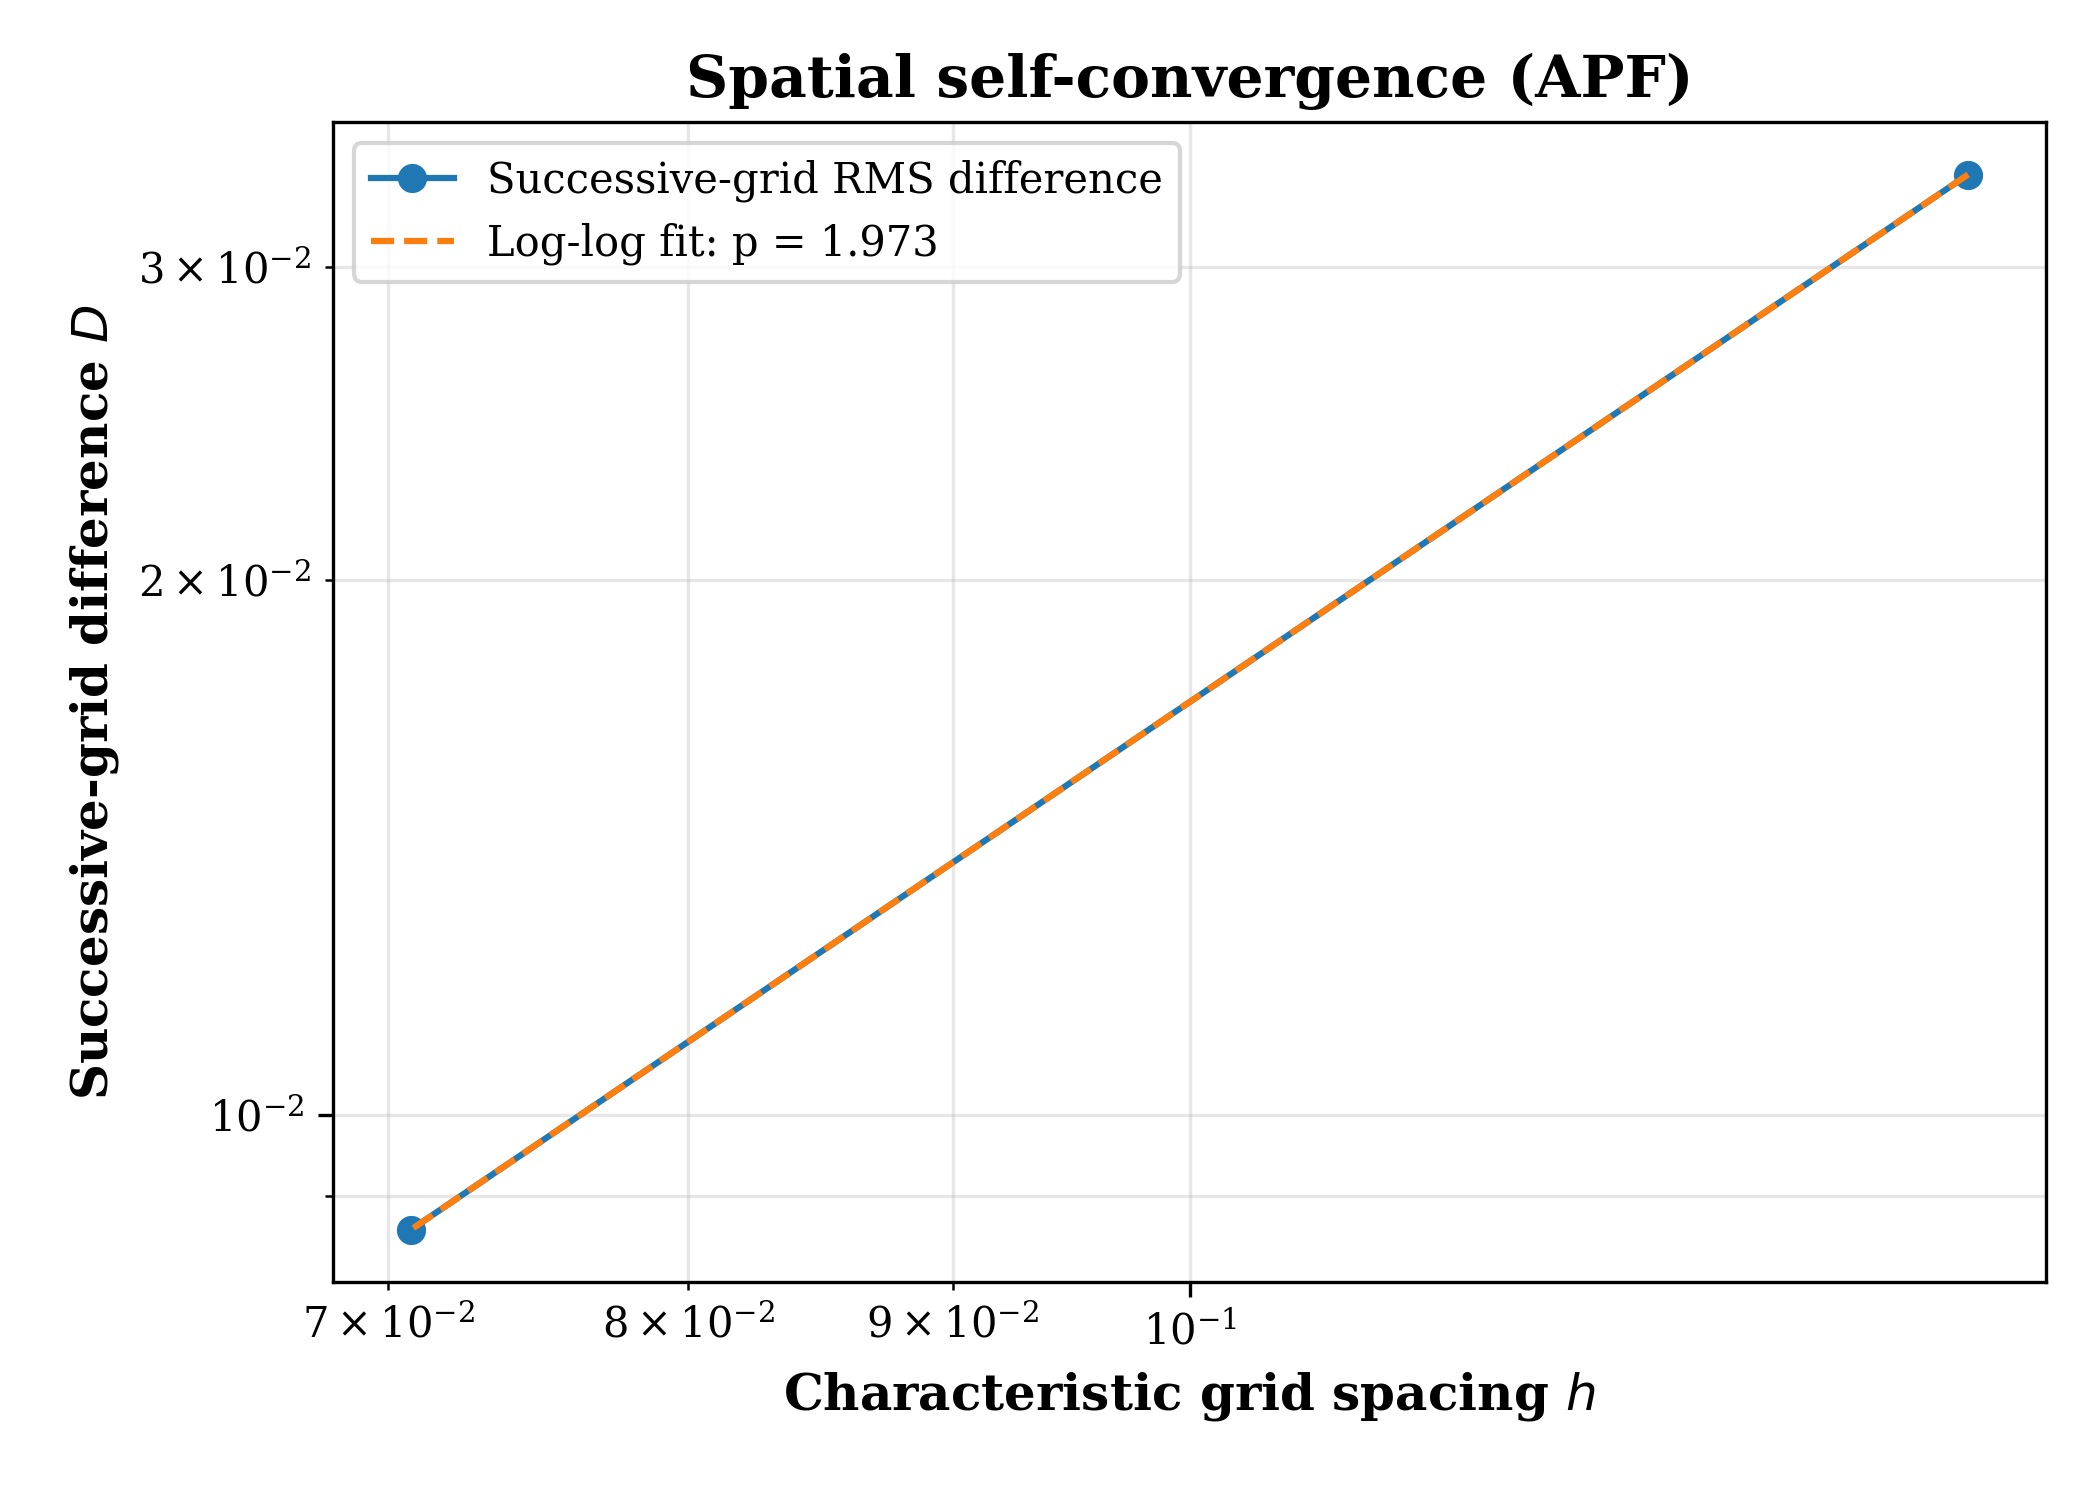
\includegraphics[width=\linewidth]
    {figures/grid_self_convergence_APF.png}

    {\small (a) APF}
\end{minipage}
\hfill
\begin{minipage}[t]{0.48\textwidth}
    \centering
    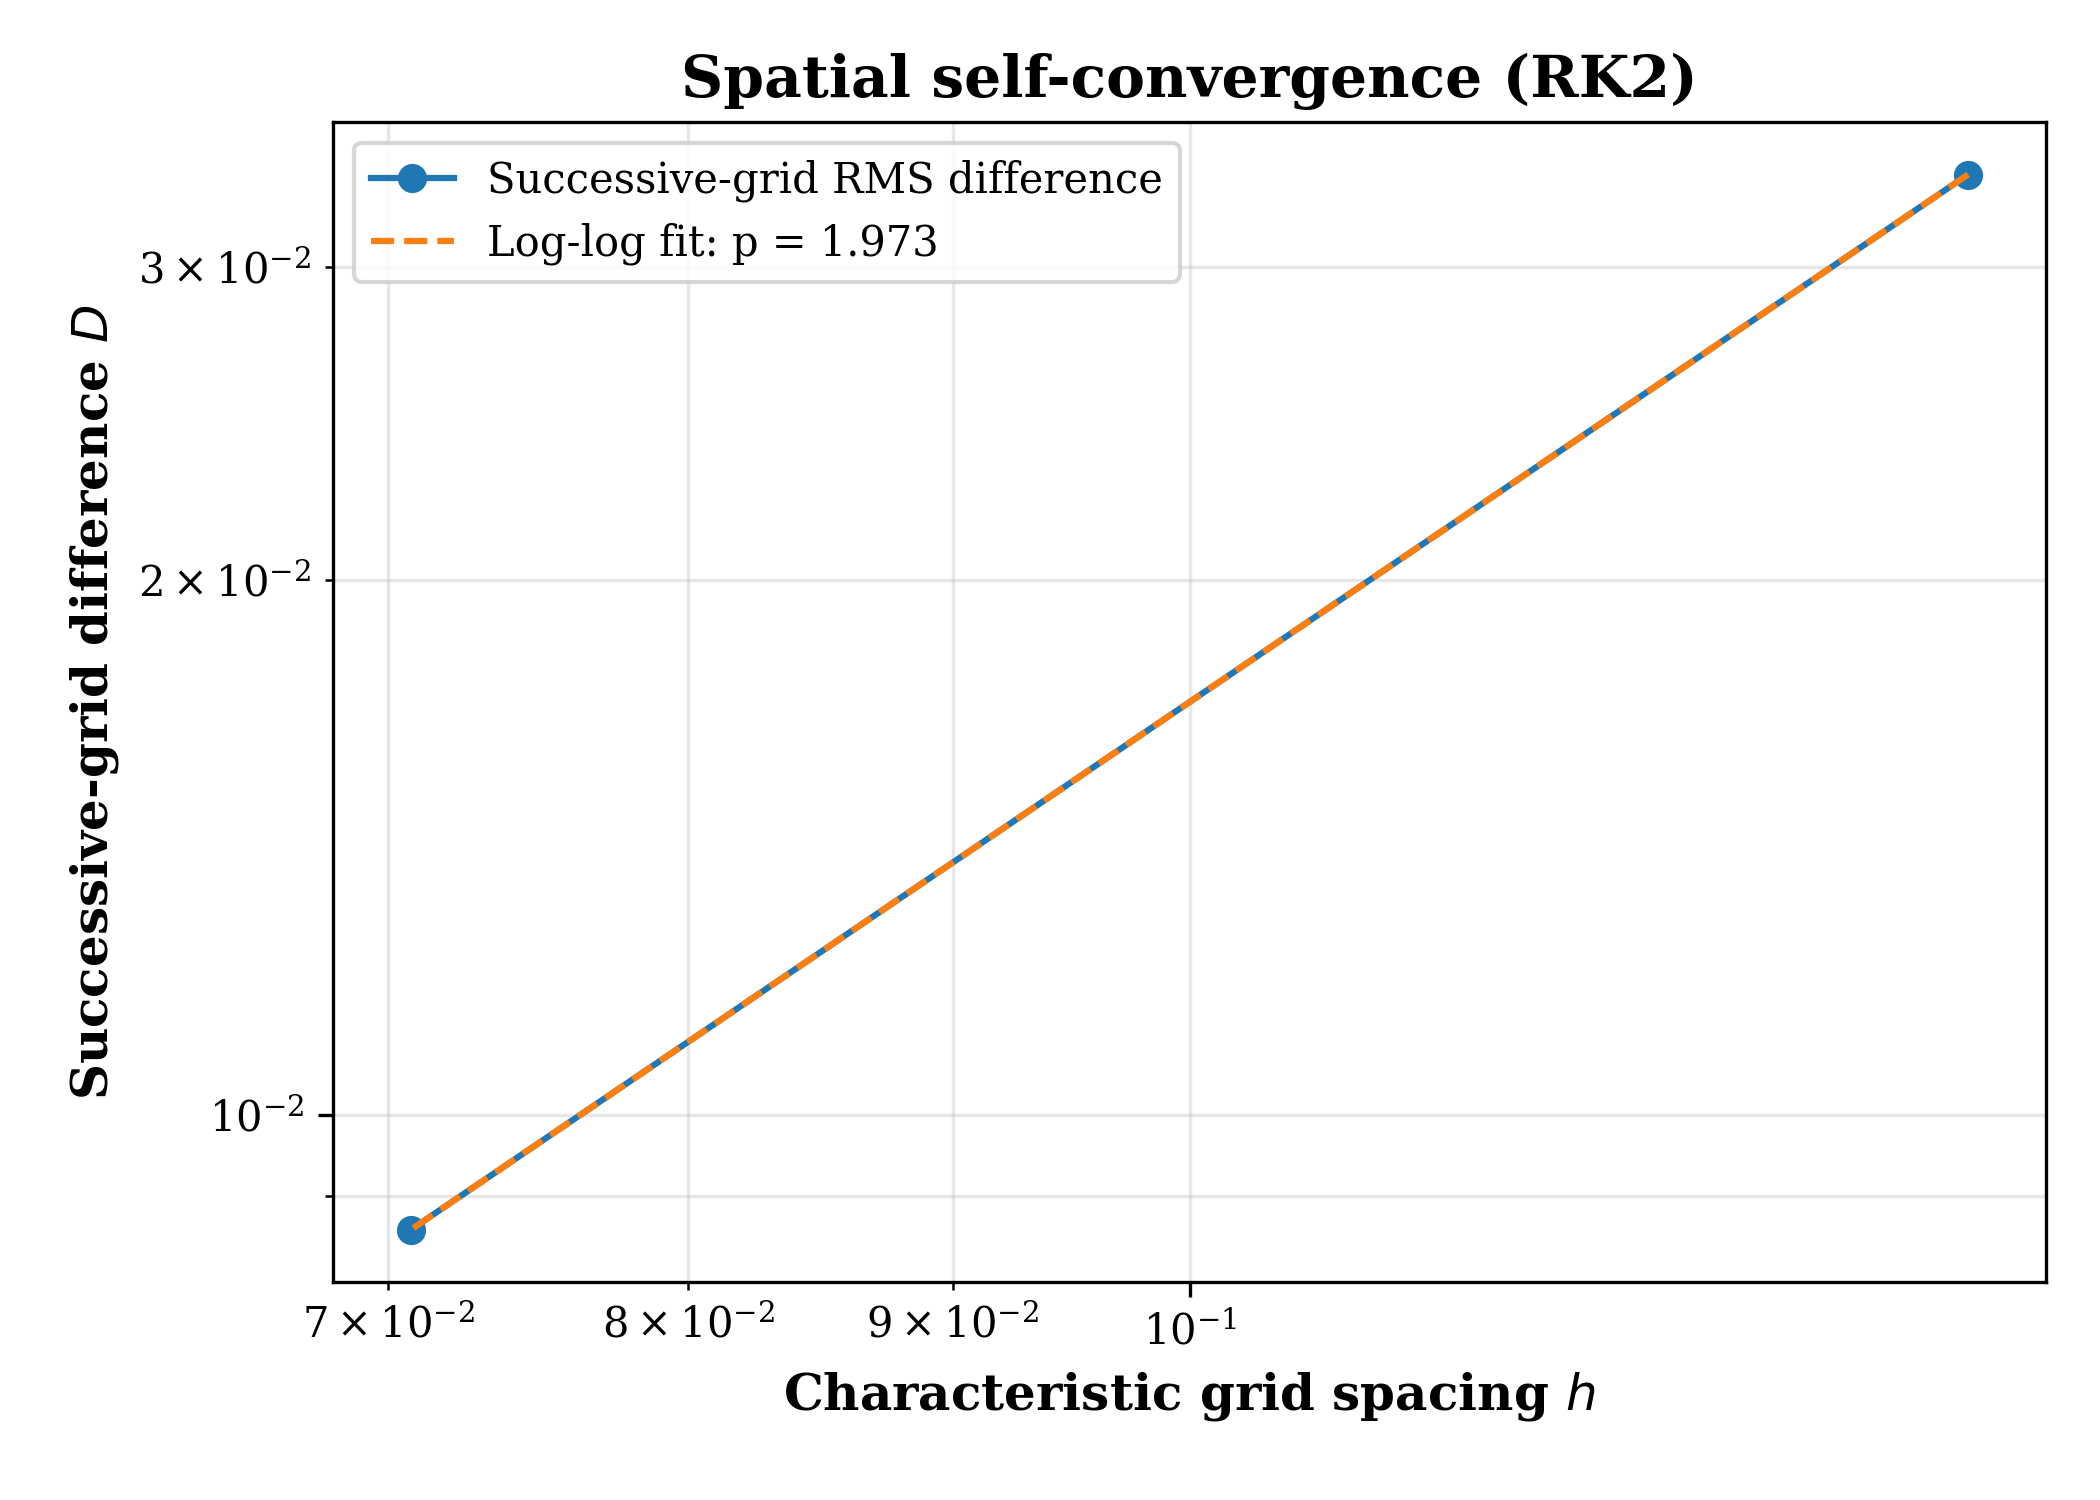
\includegraphics[width=\linewidth]
    {figures/grid_self_convergence_RK2.png}

    {\small (b) Explicit midpoint RK2}
\end{minipage}

\vspace{0.4cm}

\begin{minipage}[t]{0.48\textwidth}
    \centering
    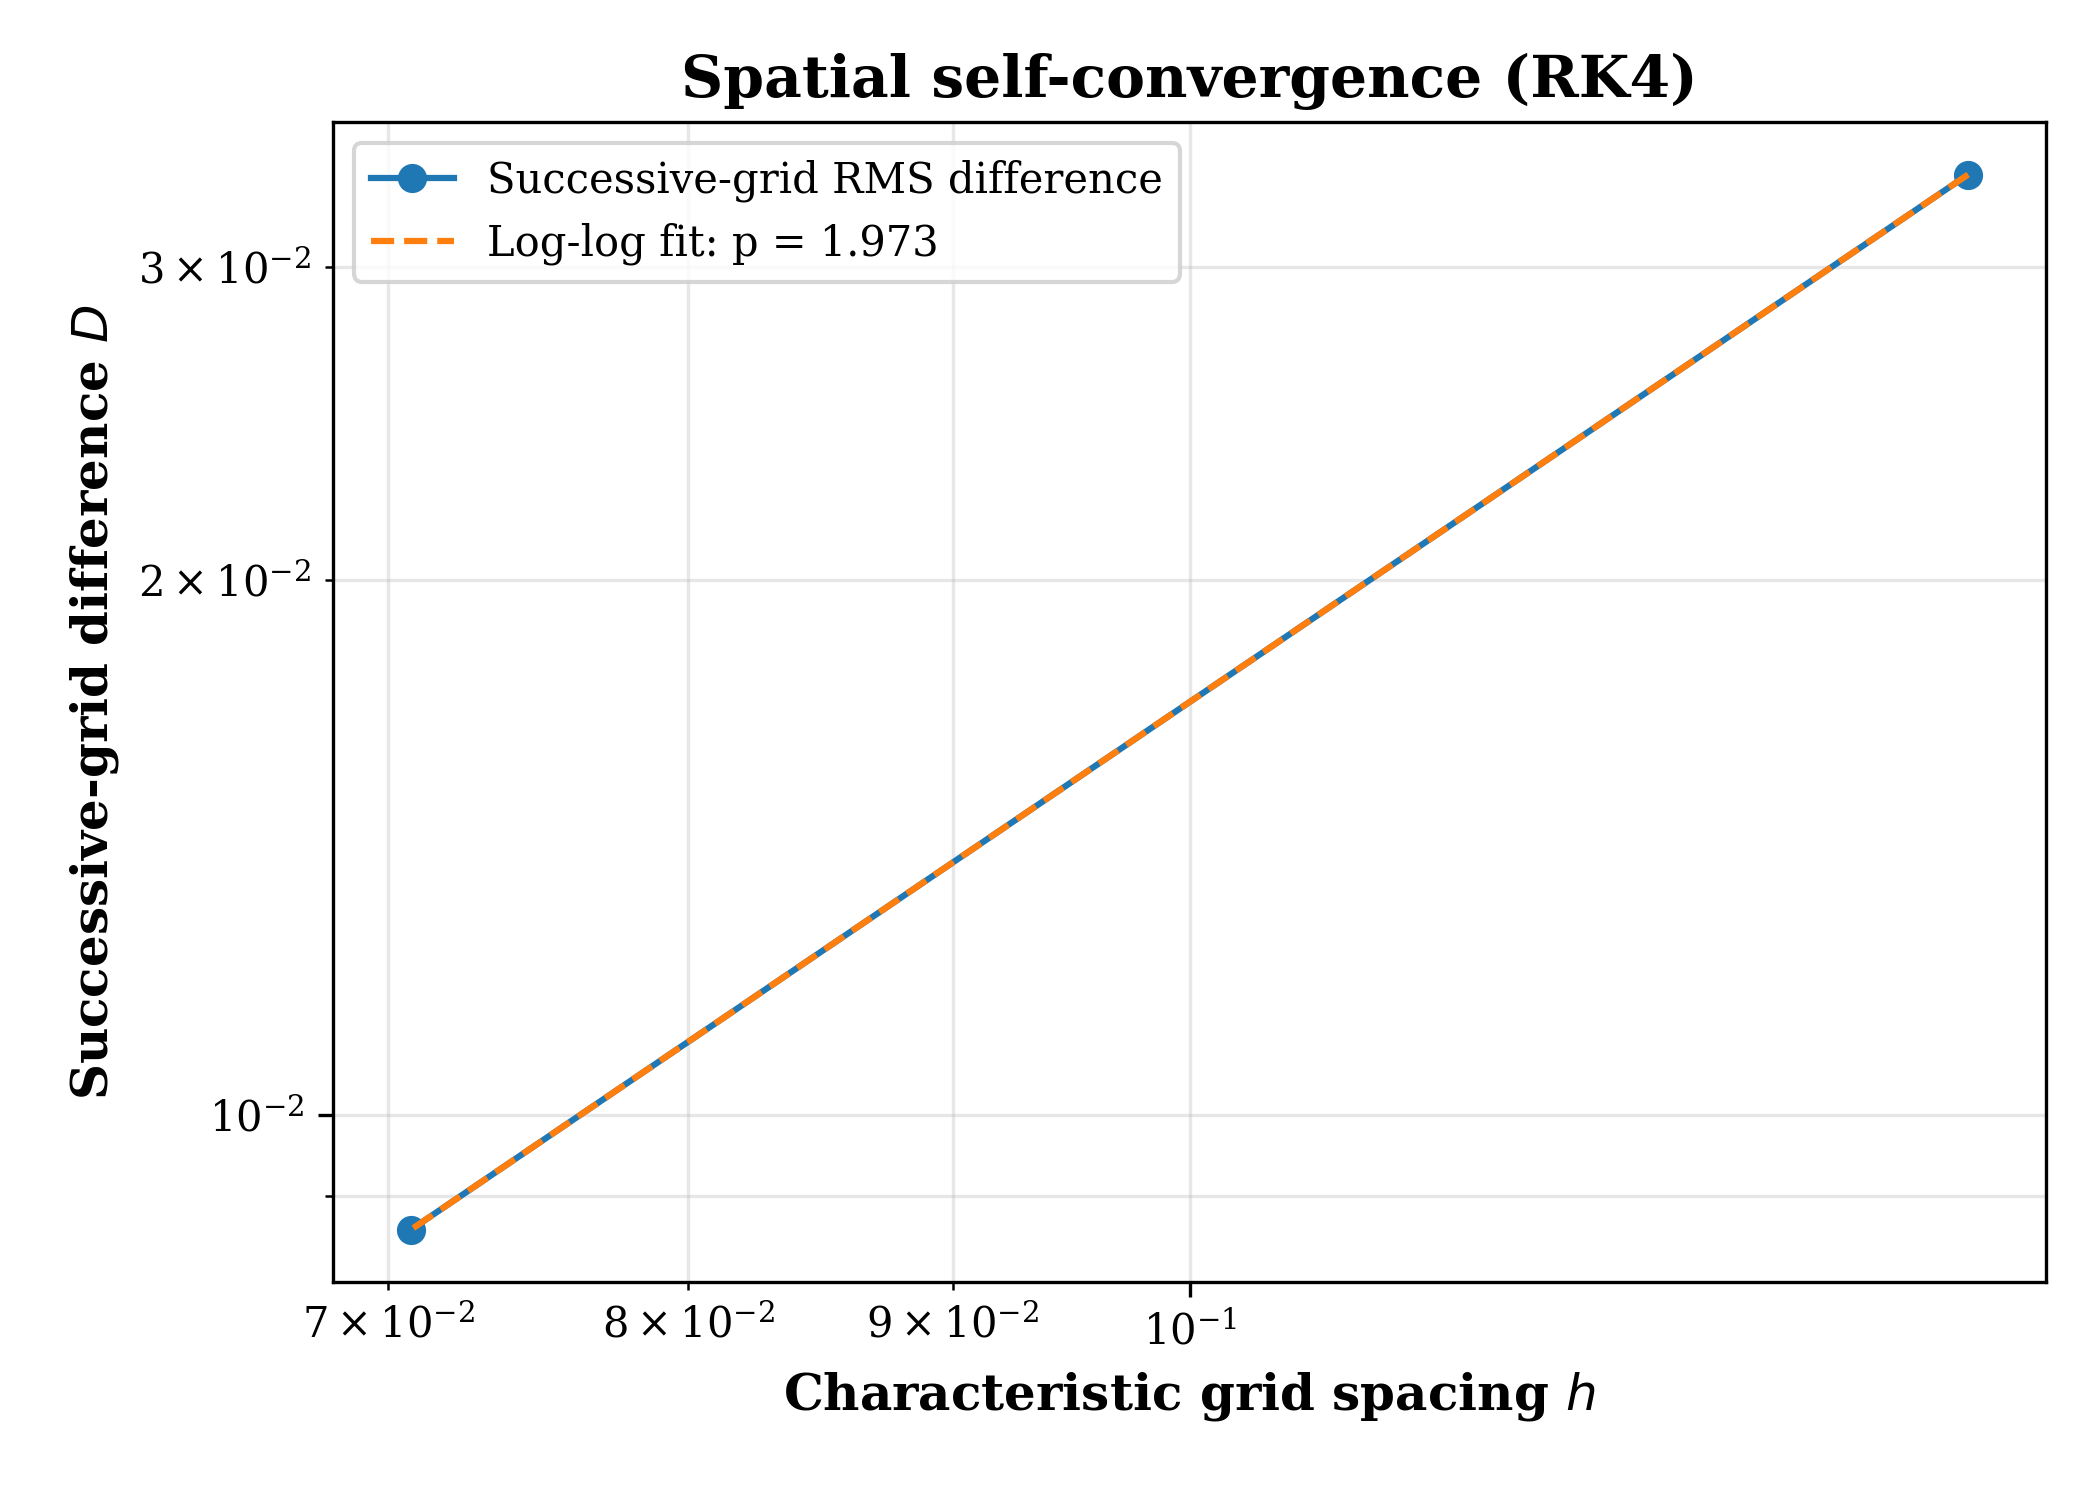
\includegraphics[width=\linewidth]
    {figures/grid_self_convergence_RK4.png}

    {\small (c) Classical RK4}
\end{minipage}
\hfill
\begin{minipage}[t]{0.48\textwidth}
    \centering
    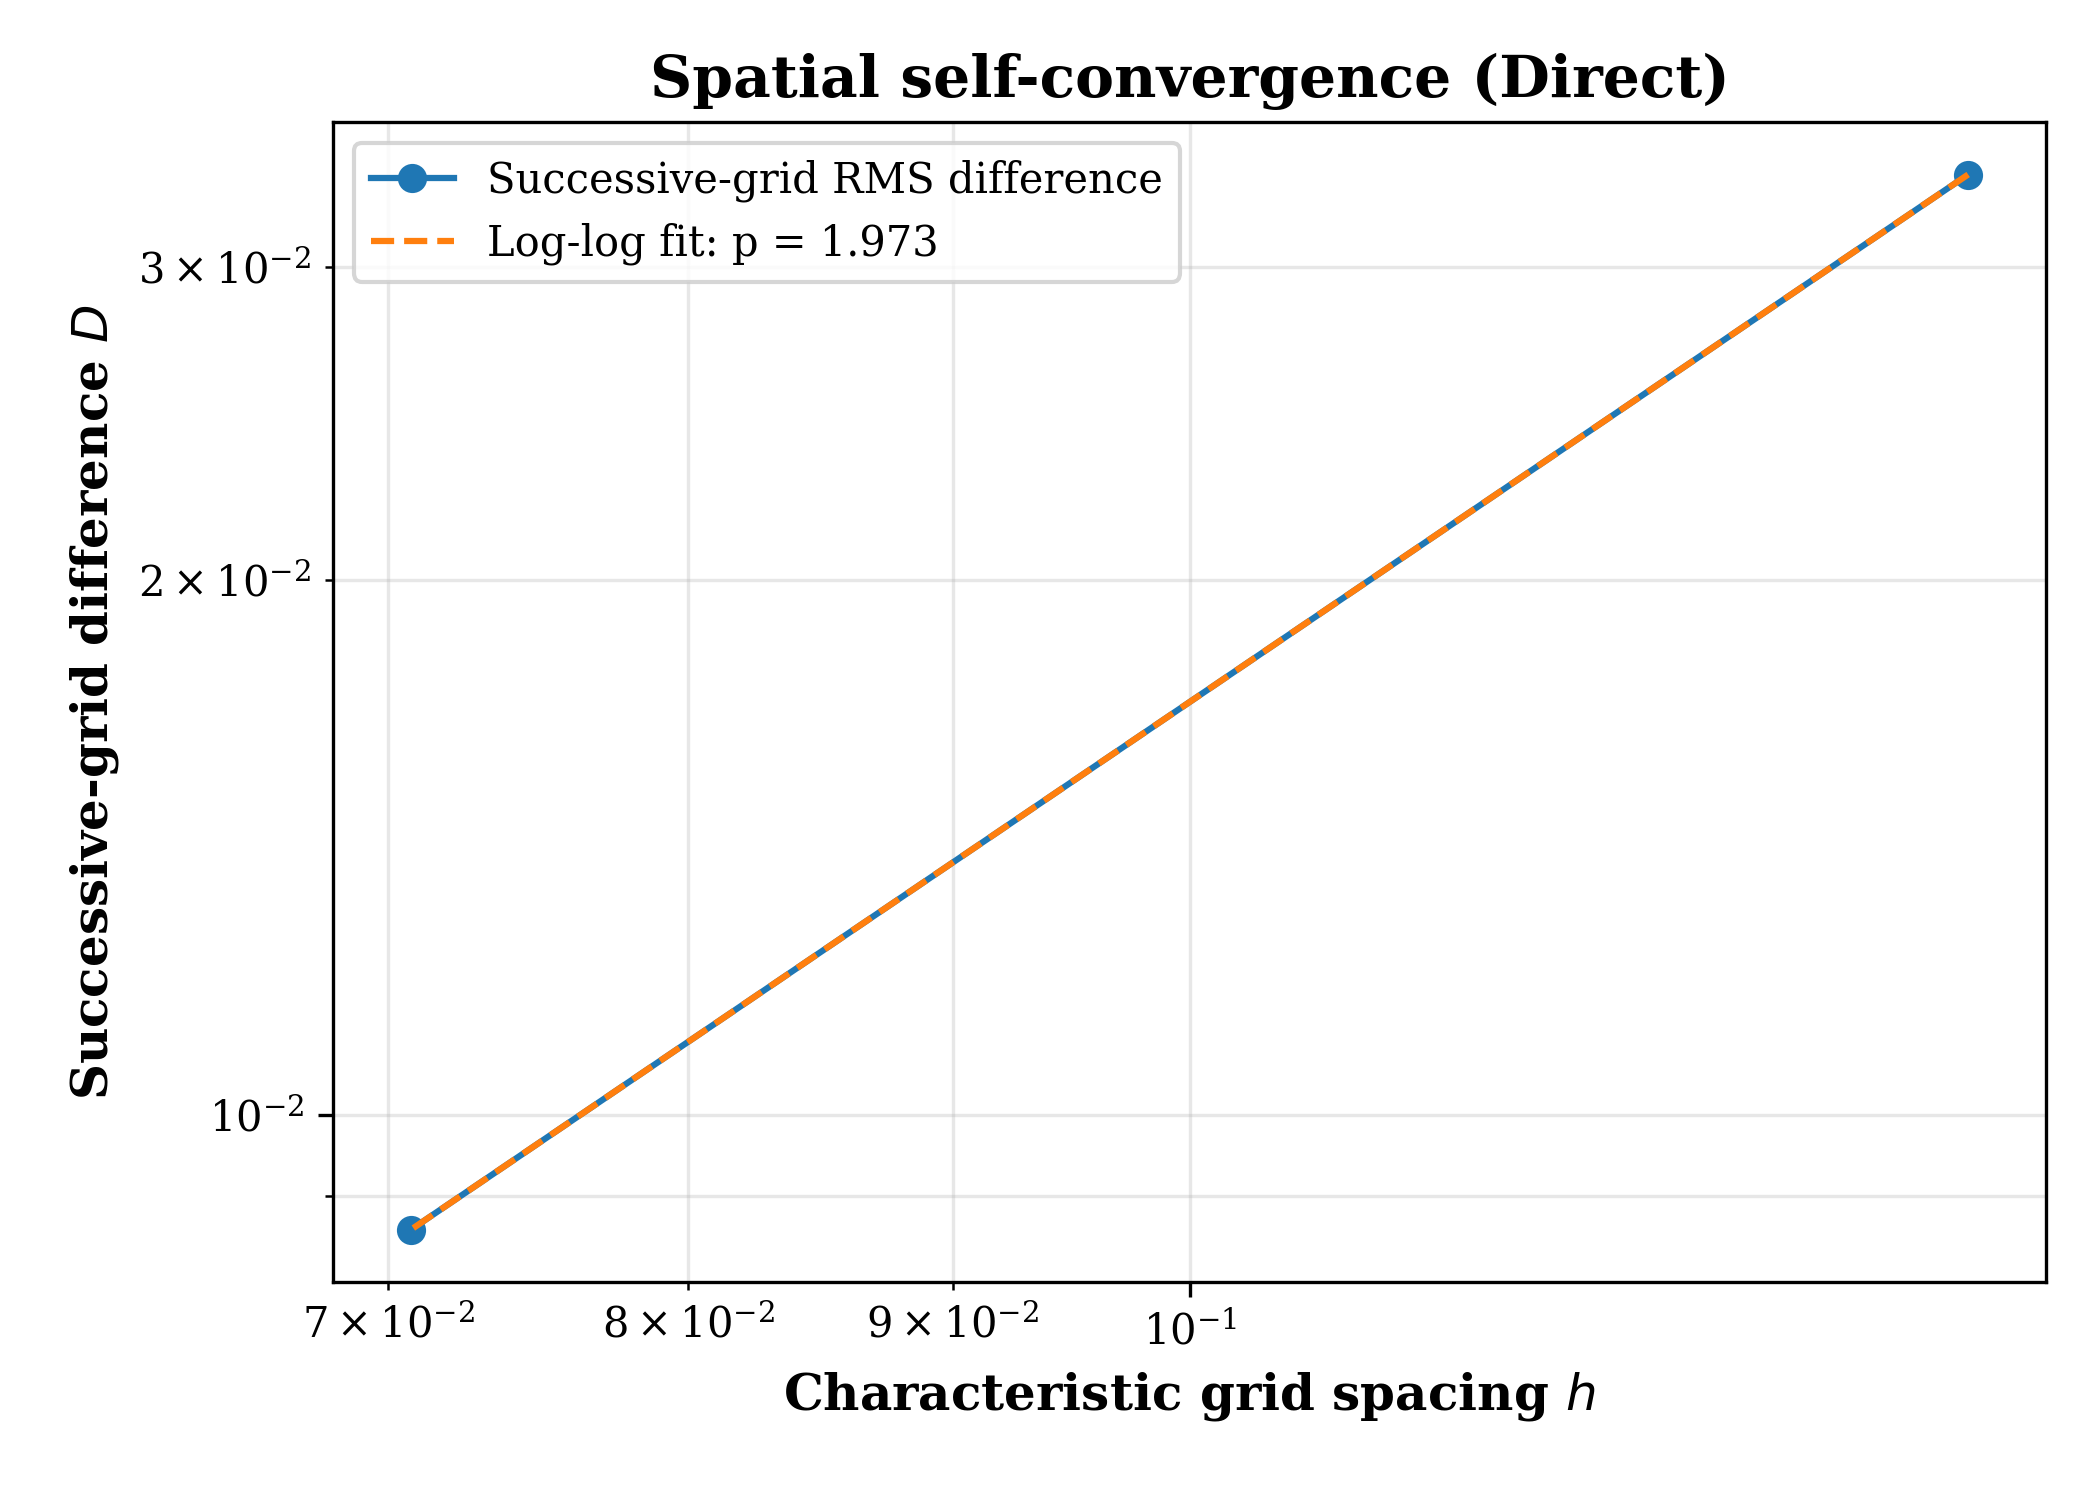
\includegraphics[width=\linewidth]
    {figures/grid_self_convergence_Direct.png}

    {\small (d) Direct implicit Euler}
\end{minipage}

\caption{Spatial self-convergence of the four numerical
methods for the linear inlet condition. Successive-grid
RMS differences are plotted against characteristic grid
spacing on logarithmic axes. All methods yield an observed
spatial convergence order of approximately two.}
\label{fig:all_solver_grid_convergence}
\end{figure}

Overall, the results demonstrate consistent second-order
spatial self-convergence across all four numerical methods.
The agreement in successive-grid differences also supports
the consistency of their implementations and their
convergence toward a common discrete steady-state solution.
However, self-convergence does not independently establish
the absolute error of the finest-grid solution.

\subsection{Temporal Accuracy Assessment}
\label{subsec:temporal_accuracy}

Temporal accuracy is assessed through a self-convergence study
in which the spatial grid and integration horizon are kept
fixed while the pseudo-time step is successively reduced.
For each time step, the solver advances the initial temperature
field over the same total pseudo-time interval. This allows
the differences between the resulting temperature fields to
be attributed primarily to temporal discretization.

The computational domain is discretized using a fixed grid
of $25\times10$ cells. The initial time step is
$\Delta t_0=0.05$, and three successive halvings are applied,
giving four time-step levels:
\begin{equation}
\Delta t_\ell=\frac{\Delta t_0}{2^\ell},
\qquad \ell=0,1,2,3.
\label{eq:temporal_step_refinement}
\end{equation}

All calculations are performed over the same final pseudo-time
$\tau_f=0.5$. Consequently, the required number of iterations
for each time step is
\begin{equation}
N_\ell=\frac{\tau_f}{\Delta t_\ell},
\label{eq:temporal_iteration_count}
\end{equation}
which gives $10$, $20$, $40$, and $80$ iterations,
respectively.

To ensure that every calculation reaches the same integration
horizon, residual-based early termination is disabled by
setting the residual tolerance to zero. The maximum iteration
count is set equal to the required number of time steps, and
the actual number of iterations is checked after each run.

\subsubsection{Successive-Time-Step Differences}

Since all solutions are obtained on the same spatial grid,
their physical-cell temperature fields can be compared
directly, without spatial interpolation. Ghost cells are
excluded from the comparison.

The RMS difference between solutions obtained using two
successive time steps is defined as
\begin{equation}
D_{\ell,\ell+1}
=
\sqrt{
\frac{1}{n_xn_y}
\sum_{i=1}^{n_x}
\sum_{j=1}^{n_y}
\left(
T_{ij}^{\Delta t_\ell}
-
T_{ij}^{\Delta t_{\ell+1}}
\right)^2
},
\label{eq:temporal_difference_norm}
\end{equation}
where both solutions correspond to the same final pseudo-time
and spatial grid.

\subsubsection{Observed Temporal Convergence Order}

Assuming that the numerical solutions are in the asymptotic
temporal convergence range, the successive-time-step
differences approximately satisfy
\begin{equation}
D_{\ell,\ell+1}\propto(\Delta t_\ell)^p,
\label{eq:temporal_difference_scaling}
\end{equation}
where $p$ is the observed temporal order of convergence.

Since each time-step refinement reduces $\Delta t$ by a
factor of two, the observed order between successive
difference estimates is
\begin{equation}
\boxed{
p_{\mathrm{obs},\ell}
=
\frac{
\ln\left(D_{\ell,\ell+1}/D_{\ell+1,\ell+2}\right)
}{
\ln 2
}.
}
\label{eq:observed_temporal_order}
\end{equation}

In addition to the pairwise estimates, a fitted temporal
order is obtained through a least-squares linear fit of
$\ln D_{\ell,\ell+1}$ against $\ln\Delta t_\ell$:
\begin{equation}
\ln D_{\ell,\ell+1}
=
p_{\mathrm{fit}}\ln\Delta t_\ell+C,
\label{eq:temporal_log_fit}
\end{equation}
where $p_{\mathrm{fit}}$ is the fitted slope and $C$ is
the intercept.

\begin{algorithm}[H]
\caption{Temporal Self-Convergence Analysis}
\label{alg:temporal_self_convergence}
\begin{algorithmic}[1]
\Require Fixed mesh $M$, initial time step $\Delta t_0$,
number of time-step levels $N_{\Delta t}=4$, final
pseudo-time $\tau_f$, solver, and physical parameters
\Ensure Successive-time-step differences, observed and
fitted temporal orders, and convergence diagnostics

\State Generate the time-step sequence using
Equation~\eqref{eq:temporal_step_refinement}
\State Initialize solution and diagnostic records

\For{each time step $\Delta t_\ell$}
    \State Calculate the required iteration count
    $N_\ell$ using Equation~\eqref{eq:temporal_iteration_count}
    \State Initialize the temperature and velocity fields
    on the fixed mesh
    \State Set residual tolerance to zero and maximum
    iterations to $N_\ell$
    \State Execute the selected solver
    \State Verify that exactly $N_\ell$ iterations were performed
    \State Check that the final temperature field contains
    only finite values
    \State Store the final temperature field, residual,
    iteration count, and computation time
\EndFor

\For{each pair of successive time steps}
    \State Extract physical-cell temperatures from both solutions
    \State Calculate the RMS difference using
    Equation~\eqref{eq:temporal_difference_norm}
    \State Store the resulting difference
\EndFor

\For{each pair of successive difference estimates}
    \State Calculate the observed temporal order using
    Equation~\eqref{eq:observed_temporal_order}
\EndFor

\State Fit $\ln D_{\ell,\ell+1}$ against
$\ln\Delta t_\ell$ using least squares
\State Record the fitted slope $p_{\mathrm{fit}}$
\State Generate the log--log temporal self-convergence plot
\State Save time steps, differences, observed orders,
fitted order, residuals, iteration counts, and computation times
\State \Return temporal convergence results and diagnostics
\end{algorithmic}
\end{algorithm}

The temporal self-convergence study provides an estimate of
the time-integration accuracy without requiring an exact
transient solution. Its reliability depends on comparing
solutions at the same integration horizon, using sufficiently
fine time steps to reach the asymptotic convergence range.

\subsubsection{Temporal Accuracy Results}
\label{subsec:temporal_accuracy_results}

The temporal accuracy of the four numerical methods was
assessed on a fixed $25\times10$ spatial grid using
$\mathrm{Pe}=17.5$, $\mathrm{Br}=0.2$, and a linear inlet
temperature profile $T_{\mathrm{in}}(y)=y$. All calculations
were advanced over the same final pseudo-time $\tau_f=0.5$,
using successively halved time steps:
\begin{equation}
\Delta t=
\{0.05,\;0.025,\;0.0125,\;0.00625\}.
\end{equation}

The residual-based steady-state termination criterion was
disabled to ensure that all solutions were evaluated at the
same integration horizon. Consequently, the calculations
were performed for exactly $10$, $20$, $40$, and $80$
iterations, respectively.

The successive-time-step RMS differences and the resulting
temporal convergence orders are summarized in
Table~\ref{tab:temporal_accuracy_results}.

\begin{table}[H]
\centering
\caption{Temporal self-convergence results for the four
numerical methods.}
\label{tab:temporal_accuracy_results}
\small
\setlength{\tabcolsep}{5pt}
\renewcommand{\arraystretch}{1.3}
\resizebox{\textwidth}{!}{%
\begin{tabular}{c c c c c c c}
\hline
Method
& $D_{0,1}$
& $D_{1,2}$
& $D_{2,3}$
& $p_{\mathrm{obs},1}$
& $p_{\mathrm{obs},2}$
& $p_{\mathrm{fit}}$
\\
\hline
APF
& $4.8819\times10^{-3}$
& $2.5673\times10^{-3}$
& $1.3341\times10^{-3}$
& 0.92721
& 0.94437
& 0.93579
\\

RK2
& $9.3241\times10^{-4}$
& $2.1548\times10^{-4}$
& $5.2779\times10^{-5}$
& 2.11338
& 2.02955
& 2.07147
\\

RK4
& $2.0929\times10^{-5}$
& $1.2419\times10^{-6}$
& $7.5599\times10^{-8}$
& 4.07489
& 4.03803
& 4.05646
\\

Direct
& $4.7960\times10^{-3}$
& $2.5499\times10^{-3}$
& $1.3306\times10^{-3}$
& 0.91137
& 0.93840
& 0.92488
\\
\hline
\end{tabular}%
}
\end{table}

Here, $D_{0,1}$, $D_{1,2}$, and $D_{2,3}$ denote the
RMS differences between solutions obtained using successive
time steps. The observed orders are calculated using
Equation~\eqref{eq:observed_temporal_order}, while
$p_{\mathrm{fit}}$ represents the slope of the corresponding
log--log least-squares fit.

\begin{figure}[H]
\centering

\begin{minipage}[t]{0.48\textwidth}
    \centering
    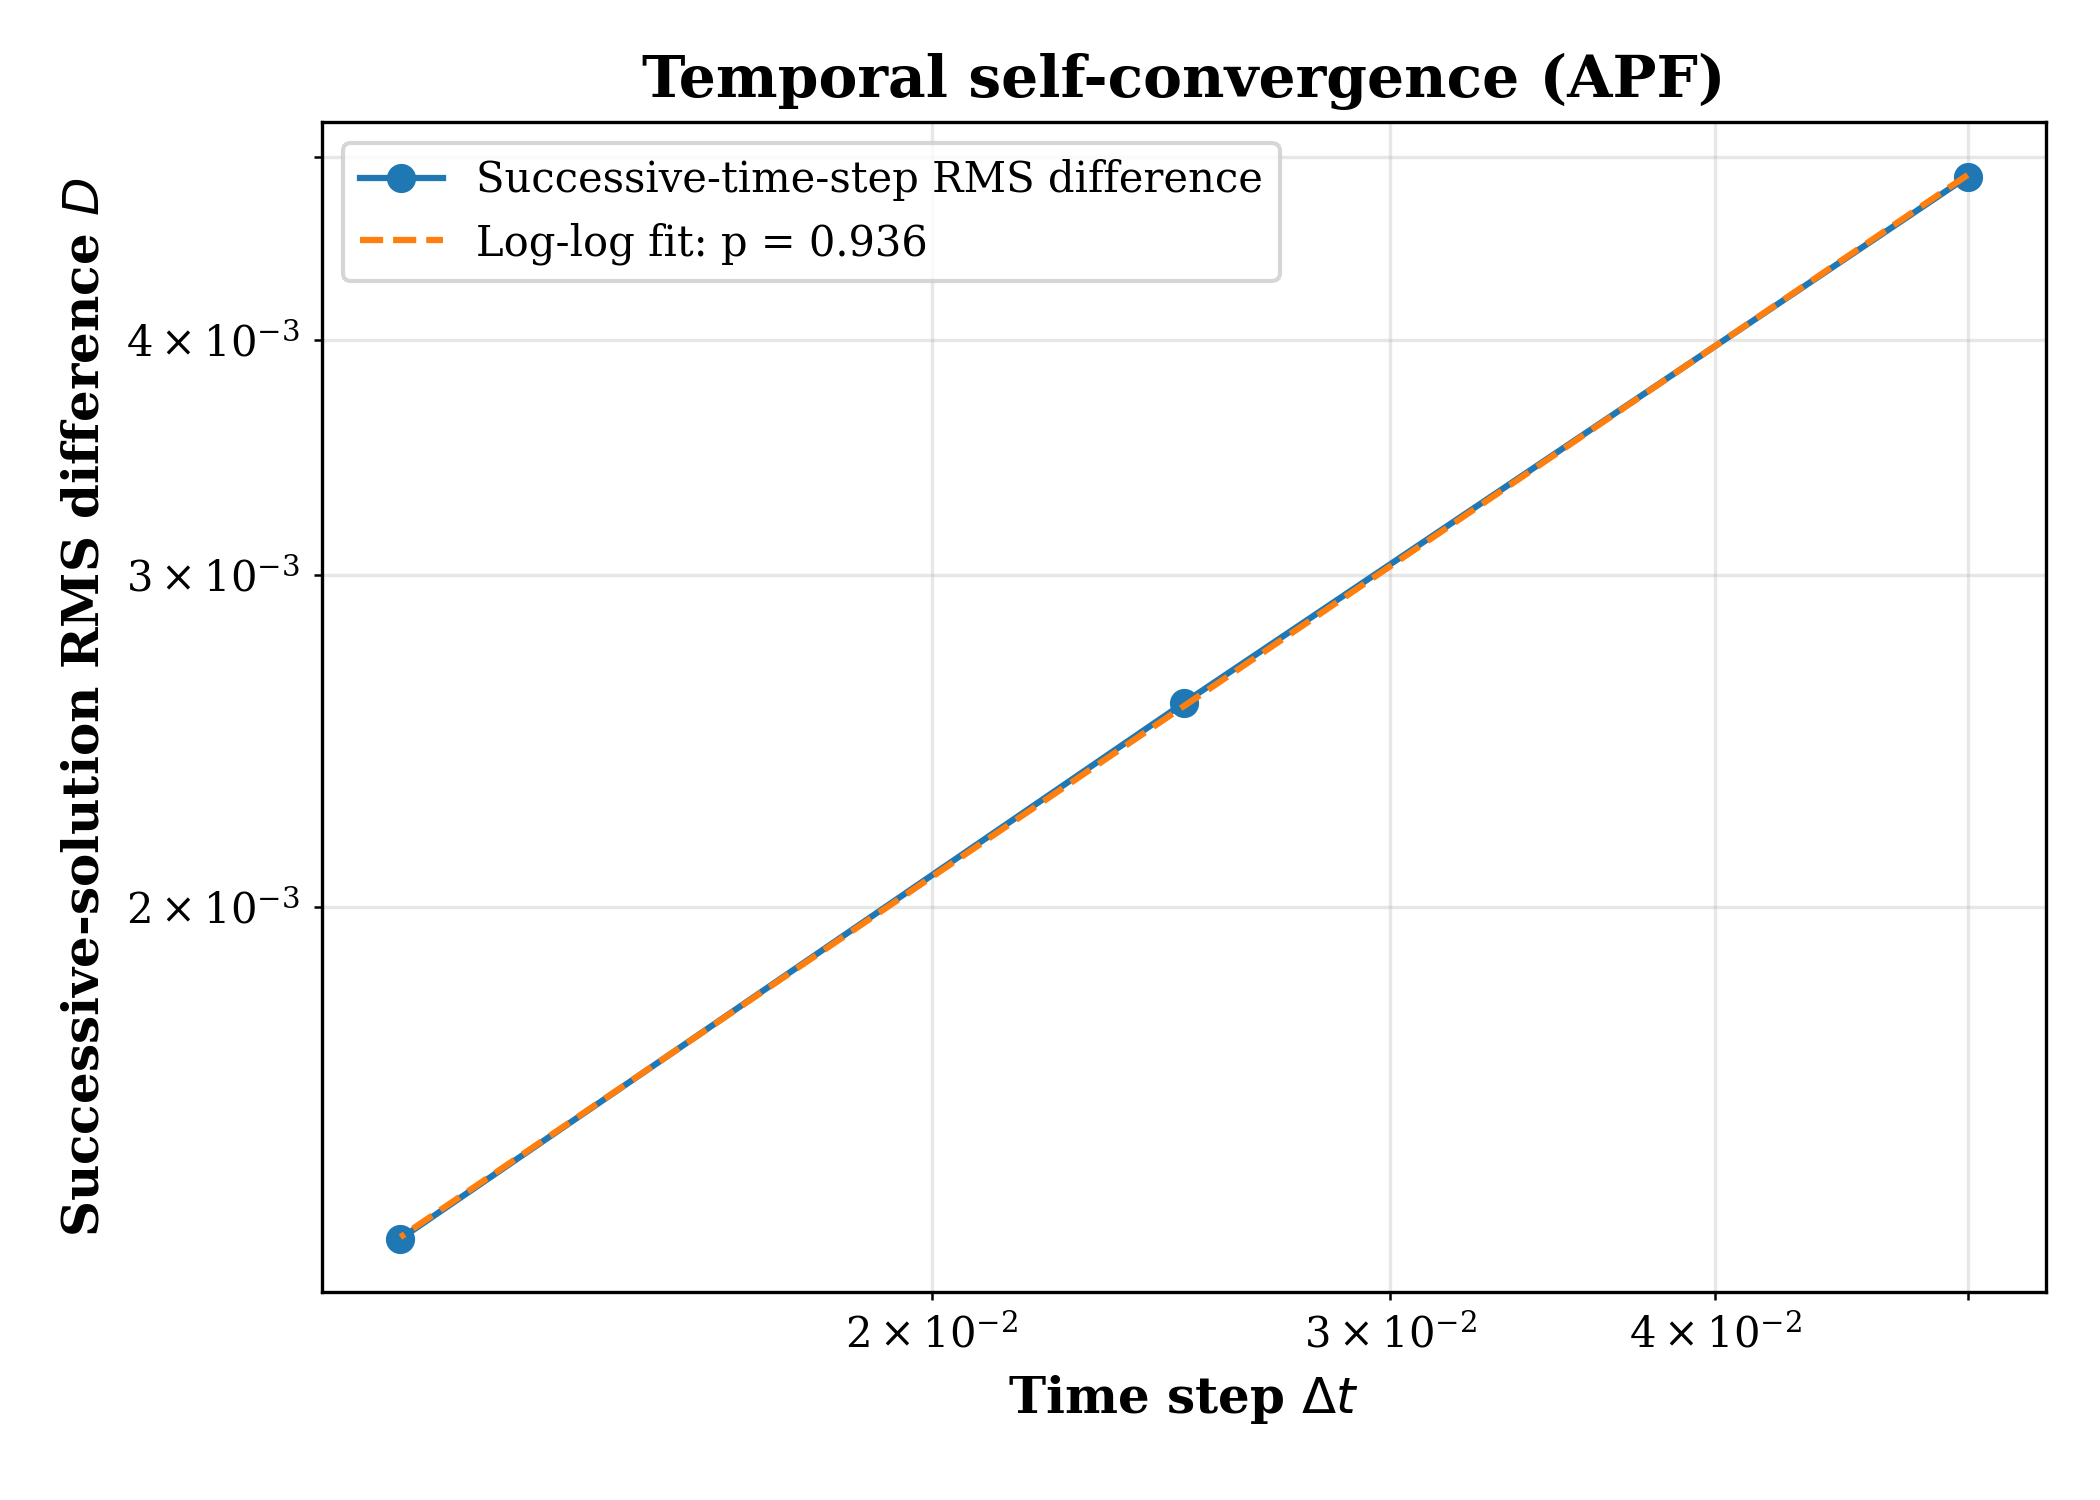
\includegraphics[width=\linewidth]
    {figures/temporal_self_convergence_APF.png}

    {\small (a) Approximate factorization (APF)}
\end{minipage}
\hfill
\begin{minipage}[t]{0.48\textwidth}
    \centering
    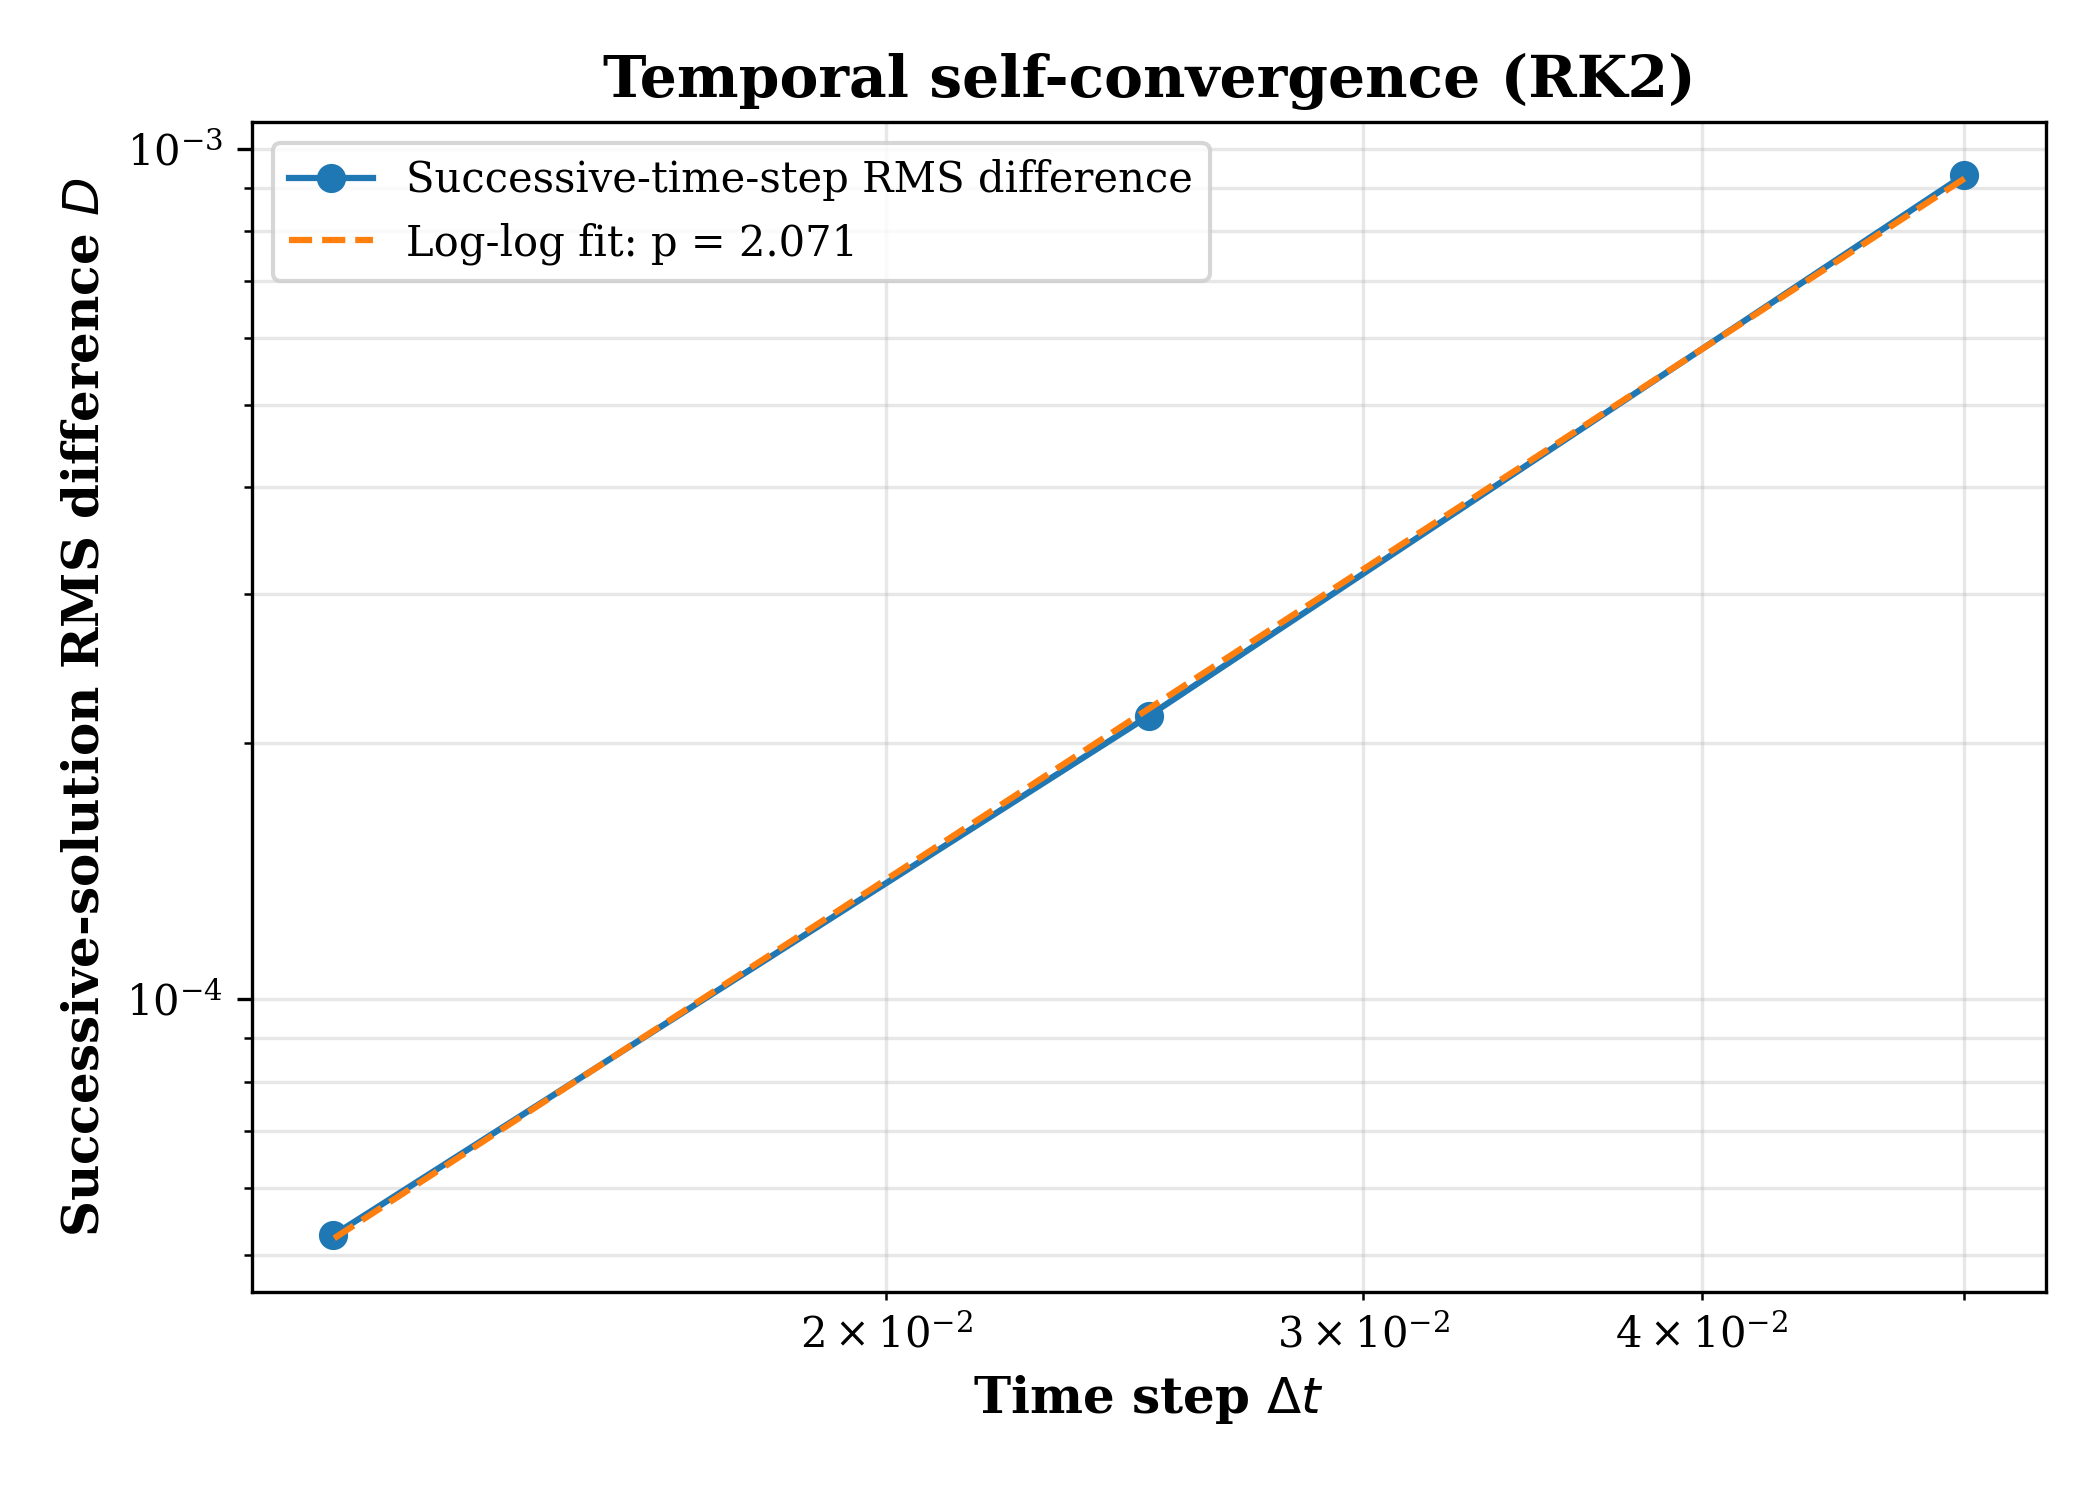
\includegraphics[width=\linewidth]
    {figures/temporal_self_convergence_RK2.png}

    {\small (b) Explicit midpoint RK2}
\end{minipage}

\vspace{0.4cm}

\begin{minipage}[t]{0.48\textwidth}
    \centering
    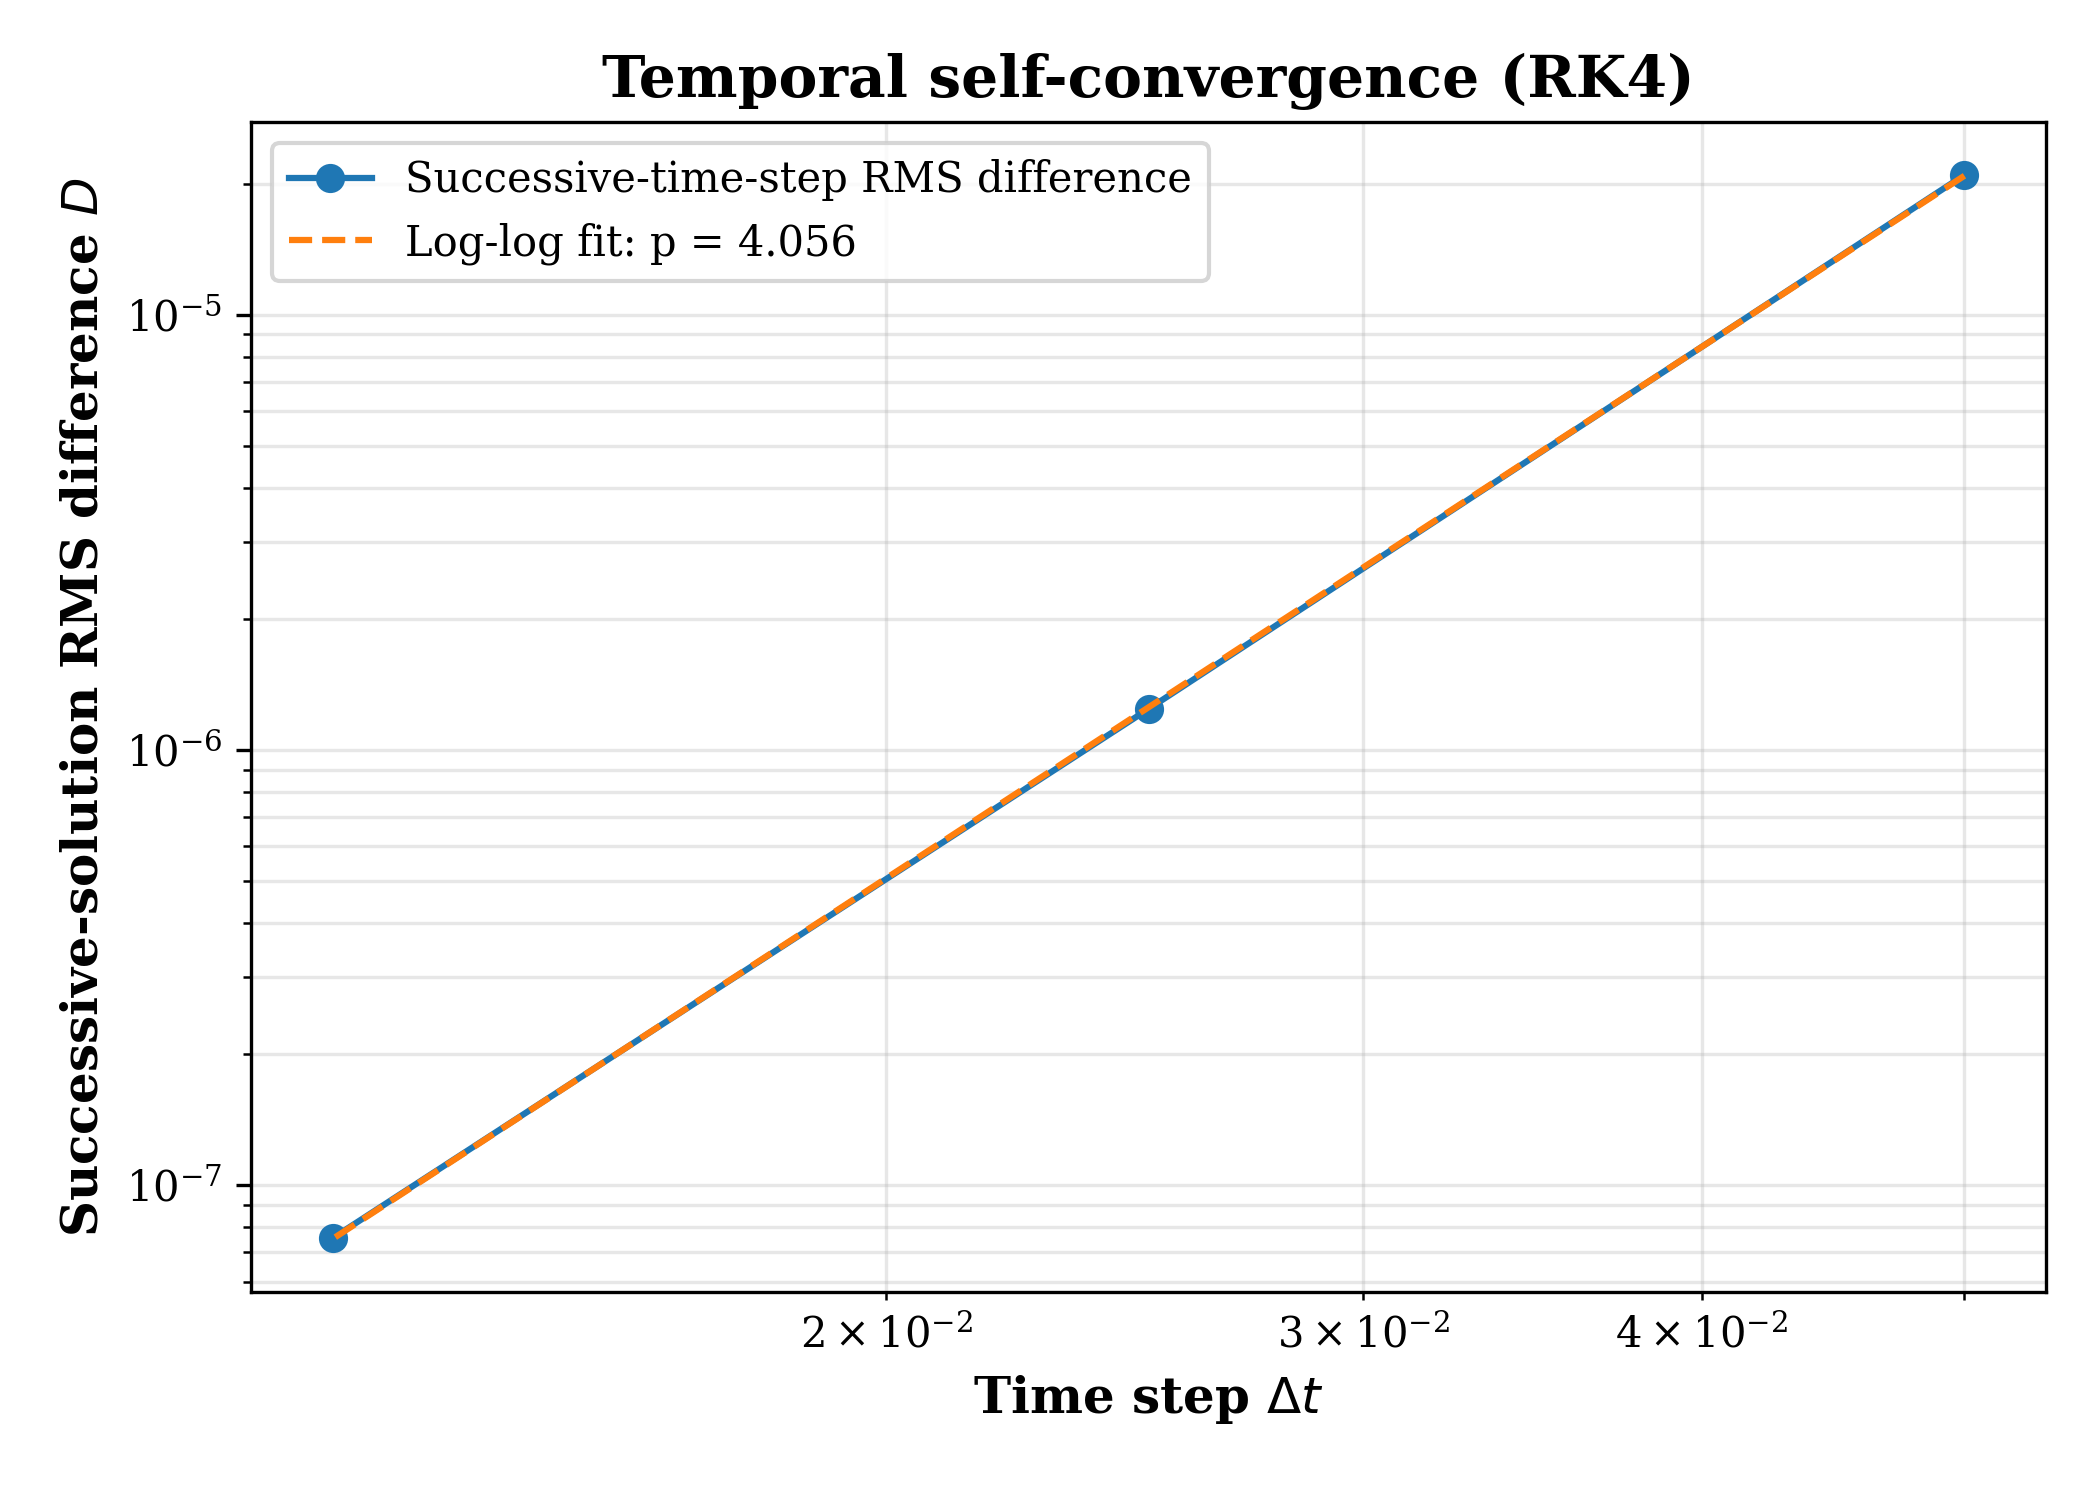
\includegraphics[width=\linewidth]
    {figures/temporal_self_convergence_RK4.png}

    {\small (c) Classical RK4}
\end{minipage}
\hfill
\begin{minipage}[t]{0.48\textwidth}
    \centering
    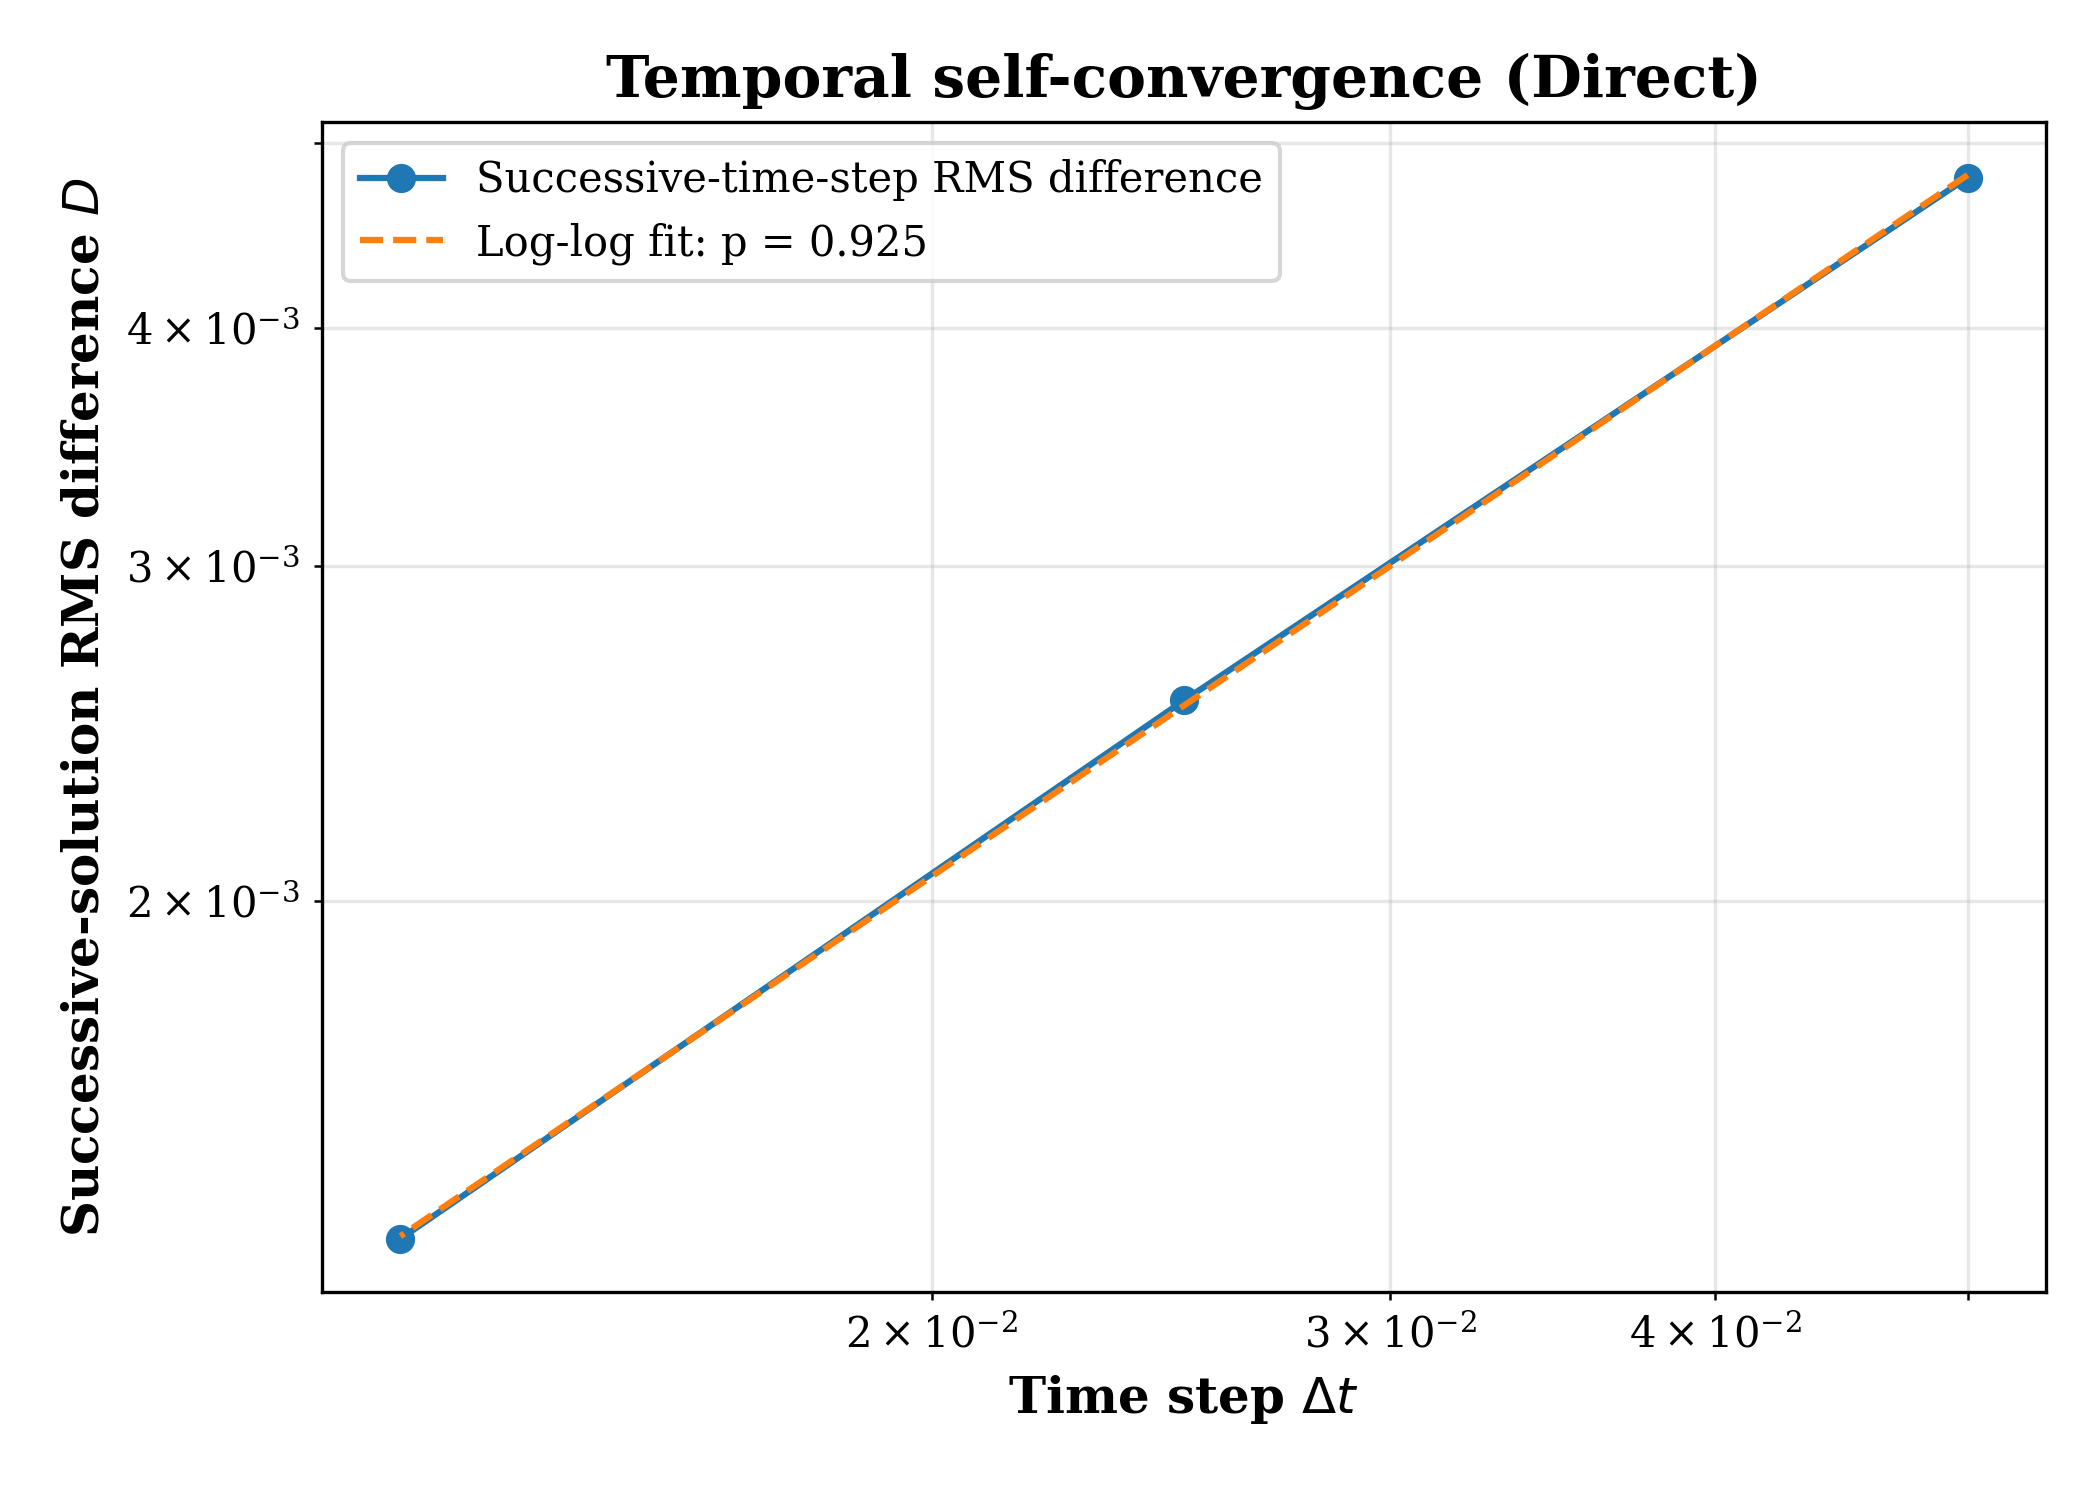
\includegraphics[width=\linewidth]
    {figures/temporal_self_convergence_Direct.png}

    {\small (d) Direct implicit Euler}
\end{minipage}

\caption{Temporal self-convergence of the four numerical
methods on the fixed $25\times10$ grid. Successive-time-step
RMS differences are plotted against the time step on
logarithmic axes.}
\label{fig:temporal_self_convergence}
\end{figure}

The results indicate approximately first-order temporal
convergence for both APF and the direct implicit Euler method,
with fitted orders of $0.93579$ and $0.92488$, respectively.
The explicit midpoint method exhibits approximately
second-order convergence, with a fitted order of $2.07147$.
The classical fourth-order Runge--Kutta method achieves a
fitted order of $4.05646$. These estimates are consistent
with the expected temporal accuracy of the respective
integration schemes.

The successive-difference values also decrease systematically
as the time step is refined. In particular, the RK4 method
exhibits substantially smaller differences than the other
methods for the tested time-step range, consistent with its
higher temporal order. The pairwise estimates for all methods
are reasonably close to their respective theoretical orders,
indicating that the selected time-step range provides a
consistent assessment of temporal convergence.

The final RMS residuals remain approximately between
$0.391$ and $0.393$ for all methods. This is expected because
the calculations are intentionally terminated at the fixed
pseudo-time $\tau_f=0.5$, before reaching steady state.
The residual values therefore characterize the transient
solution at the selected integration horizon and are not
used as a convergence criterion in this study.

Overall, the results confirm the expected temporal orders
of the four numerical methods: first order for APF and
implicit Euler, second order for explicit midpoint RK2,
and fourth order for classical RK4.

\subsection{Stability and Time-Step Efficiency}
\label{subsec:stability_time_step}

\subsubsection{Stability Analysis}

To assess the stability of the time-integration methods, the
semi-discrete system was expressed in matrix form as
\begin{equation}
    \frac{d\mathbf{T}}{dt}
    =
    \mathbf{A}\mathbf{T}+\mathbf{b},
    \label{eq:semi_discrete_matrix}
\end{equation}
where $\mathbf{A}$ represents the linear spatial discretization,
including the contributions of the boundary conditions, and
$\mathbf{b}$ contains the temperature-independent source terms.
Since the prescribed velocity field makes the viscous-dissipation
source independent of temperature, it does not affect the
eigenvalue-based stability analysis.

The eigenvalues of $\mathbf{A}$ were computed numerically for
the $50\times20$ grid. The maximum real part and maximum
eigenvalue magnitude were found to be
\begin{equation}
    \max_k \Re(\lambda_k)
    =
    -1.216672\times10^{1},
    \qquad
    \max_k |\lambda_k|
    =
    1.142857\times10^{2}.
\end{equation}
The negative real parts indicate that the semi-discrete system
is asymptotically stable.

The absolute stability of a time-integration method can be
examined by applying it to the scalar test equation
$\dot{w}=\lambda w$. Defining $z=\lambda\Delta t$, the
numerical solution takes the form
$w^{n+1}=G(z)w^n$, where stability requires
$|G(z)|\leq1$. The amplification factors for the methods
considered here are
\begin{align}
    G_{\mathrm{IE}}(z)
    &=\frac{1}{1-z},
    \\
    G_{\mathrm{RK2}}(z)
    &=1+z+\frac{z^2}{2},
    \\
    G_{\mathrm{RK4}}(z)
    &=1+z+\frac{z^2}{2}
      +\frac{z^3}{6}+\frac{z^4}{24},
\end{align}
for implicit Euler, explicit midpoint RK2, and classical
explicit RK4, respectively. For a given time step, the
stability condition is evaluated over the computed spectrum:
\begin{equation}
    \max_k \left|G(\lambda_k\Delta t)\right|
    \leq 1.
    \label{eq:modal_stability_condition}
\end{equation}

Implicit Euler is A-stable and therefore stable for the
computed spectrum, since all eigenvalues have negative
real parts. In contrast, the explicit methods have
conditional stability, and their allowable time steps
depend on the eigenvalue distribution. The maximum stable
time step for each method was estimated numerically using
the search procedure presented in
Algorithm~\ref{alg:maximum_stable_timestep}.

\begin{algorithm}[htbp]
    \caption{Numerical estimation of the maximum stable time step}
    \label{alg:maximum_stable_timestep}
    \small
    \begin{algorithmic}[1]
        \Require Eigenvalues $\{\lambda_k\}$, integration scheme,
                 initial time step $\Delta t_0$
        \Ensure Estimated maximum stable time step

        \State $\alpha \gets \max_k \Re(\lambda_k)$

        \If{$\alpha > \text{stability tolerance}$}
            \State \Return NaN
            \Comment{The semi-discrete system is unstable}
        \EndIf

        \If{scheme is implicit Euler}
            \State \Return $\infty$
            \Comment{Implicit Euler is A-stable}
        \EndIf

        \State $\Delta t_{\mathrm{low}} \gets 0$
        \State $\Delta t_{\mathrm{high}} \gets
               \max(\Delta t_0,10^{-12})$
        \State bracketed $\gets$ False

        \Comment{Bracket the stability boundary}
        \For{$m=1,\ldots,N_{\mathrm{double}}$}
            \If{$\max_k |G(\lambda_k\Delta t_{\mathrm{high}})|>1$}
                \State bracketed $\gets$ True
                \State \textbf{break}
            \EndIf
            \State $\Delta t_{\mathrm{low}}
                   \gets \Delta t_{\mathrm{high}}$
            \State $\Delta t_{\mathrm{high}}
                   \gets 2\Delta t_{\mathrm{high}}$
        \EndFor

        \If{not bracketed}
            \State \Return $\infty$
            \Comment{No instability found within the search range}
        \EndIf

        \Comment{Refine the boundary by bisection}
        \For{$m=1,\ldots,N_{\mathrm{bisect}}$}
            \State $\Delta t_{\mathrm{mid}}
                   \gets \frac{1}{2}
                   (\Delta t_{\mathrm{low}}+
                   \Delta t_{\mathrm{high}})$
            \If{$\max_k |G(\lambda_k\Delta t_{\mathrm{mid}})|
                  \leq 1$}
                \State $\Delta t_{\mathrm{low}}
                       \gets \Delta t_{\mathrm{mid}}$
            \Else
                \State $\Delta t_{\mathrm{high}}
                       \gets \Delta t_{\mathrm{mid}}$
            \EndIf
        \EndFor

        \State \Return $\Delta t_{\mathrm{low}}$
        \Comment{Return the stable side of the estimated limit}
    \end{algorithmic}
\end{algorithm}

At the configured time step $\Delta t=0.1$, the maximum
amplification factors were $0.45113$, $54.87755$, and
$516.90726$ for implicit Euler, RK2, and RK4, respectively.
Thus, implicit Euler was stable at this time step, whereas
both explicit methods were unstable. The numerical search
estimated maximum stable time steps of $0.01750$ for RK2
and $0.0243713$ for RK4. The estimated stability limit of
RK4 is therefore greater than that of RK2 for the present
spatial discretization.

The results are summarized in
Table~\ref{tab:maximum_timestep}. The implicit Euler method
has no finite absolute-stability limit for the computed
spectrum. The AFI value represents the largest tested
convergent time step, rather than a theoretically established
stability bound. The eigenvalue-based stability analysis
for implicit Euler should also not be interpreted as a
formal stability result for AFI, which uses approximate
factorization and was assessed separately through numerical
convergence tests.

\begin{table}[htbp]
    \centering
    \small
    \caption{Stability limits and selected pseudo-time steps
    for the numerical methods.}
    \label{tab:maximum_timestep}
    \begin{tabular}{@{}l c p{3.0cm} p{5.0cm}@{}}
        \hline
        Method
        & $\max_k |G|$ at $\Delta t=0.1$
        & Maximum stable or selected $\Delta t$
        & Assessment
        \\
        \hline
        AFI
        & --
        & $0.271$ (largest tested)
        & Largest tested value for which convergence was obtained.
        \\[0.1cm]
        Direct implicit Euler
        & $0.45113$
        & No finite stability limit; $1.0$ selected
        & A-stable for the computed eigenvalue spectrum.
        \\[0.1cm]
        Explicit RK2
        & $54.87755$
        & $0.01750$ (estimated)
        & Conditionally stable; unstable at $\Delta t=0.1$.
        \\[0.1cm]
        Explicit RK4
        & $516.90726$
        & $0.0243713$ (estimated)
        & Conditionally stable; unstable at $\Delta t=0.1$.
        \\
        \hline
    \end{tabular}
\end{table}

For the direct implicit solver, a representative time step
of $\Delta t=1$ was selected for the efficiency comparison.
This choice is substantially more moderate than the very
large values identified in the preliminary time-step sweep.
It is nevertheless expected to provide strong modal damping.
In particular, for backward Euler and the computed spectrum,
\begin{equation}
    \max_k |G_{\mathrm{IE}}(\lambda_k\Delta t)|
    \leq
    \frac{1}{1-\Delta t\max_k\Re(\lambda_k)}.
\end{equation}
At $\Delta t=1$, this gives
\begin{equation}
    \max_k |G_{\mathrm{IE}}(\lambda_k)|
    \leq 0.07595.
\end{equation}
The selected time step must still be checked through the
steady-state residual to verify convergence.

These stability limits concern pseudo-time integration
toward the steady solution and do not establish the accuracy
of a physical transient simulation.

\subsubsection{Time-Step Efficiency}

A time-step efficiency study was performed for AFI and the
direct implicit solver on the $50\times20$ grid. Several
candidate time steps were tested for each method, with
three independent runs per candidate. Each run started
from the initial temperature field and was considered
converged when the steady-state residual satisfied the
prescribed tolerance of $10^{-12}$. All tested cases in
the preliminary study converged in all three runs.

For AFI, the fastest tested case used
$\Delta t=0.266$, with a median computation time of
$5.6624~\mathrm{s}$, 296 iterations, and a final residual
of $9.51\times10^{-13}$. Its runtime was only marginally
lower than that obtained with $\Delta t=0.265$, indicating
a relatively shallow minimum in the tested range rather
than a precisely established optimal time step.
Figure~\ref{fig:afi_timestep_efficiency} shows the
computation time across the tested AFI time steps.

\begin{figure}[htbp]
    \centering
    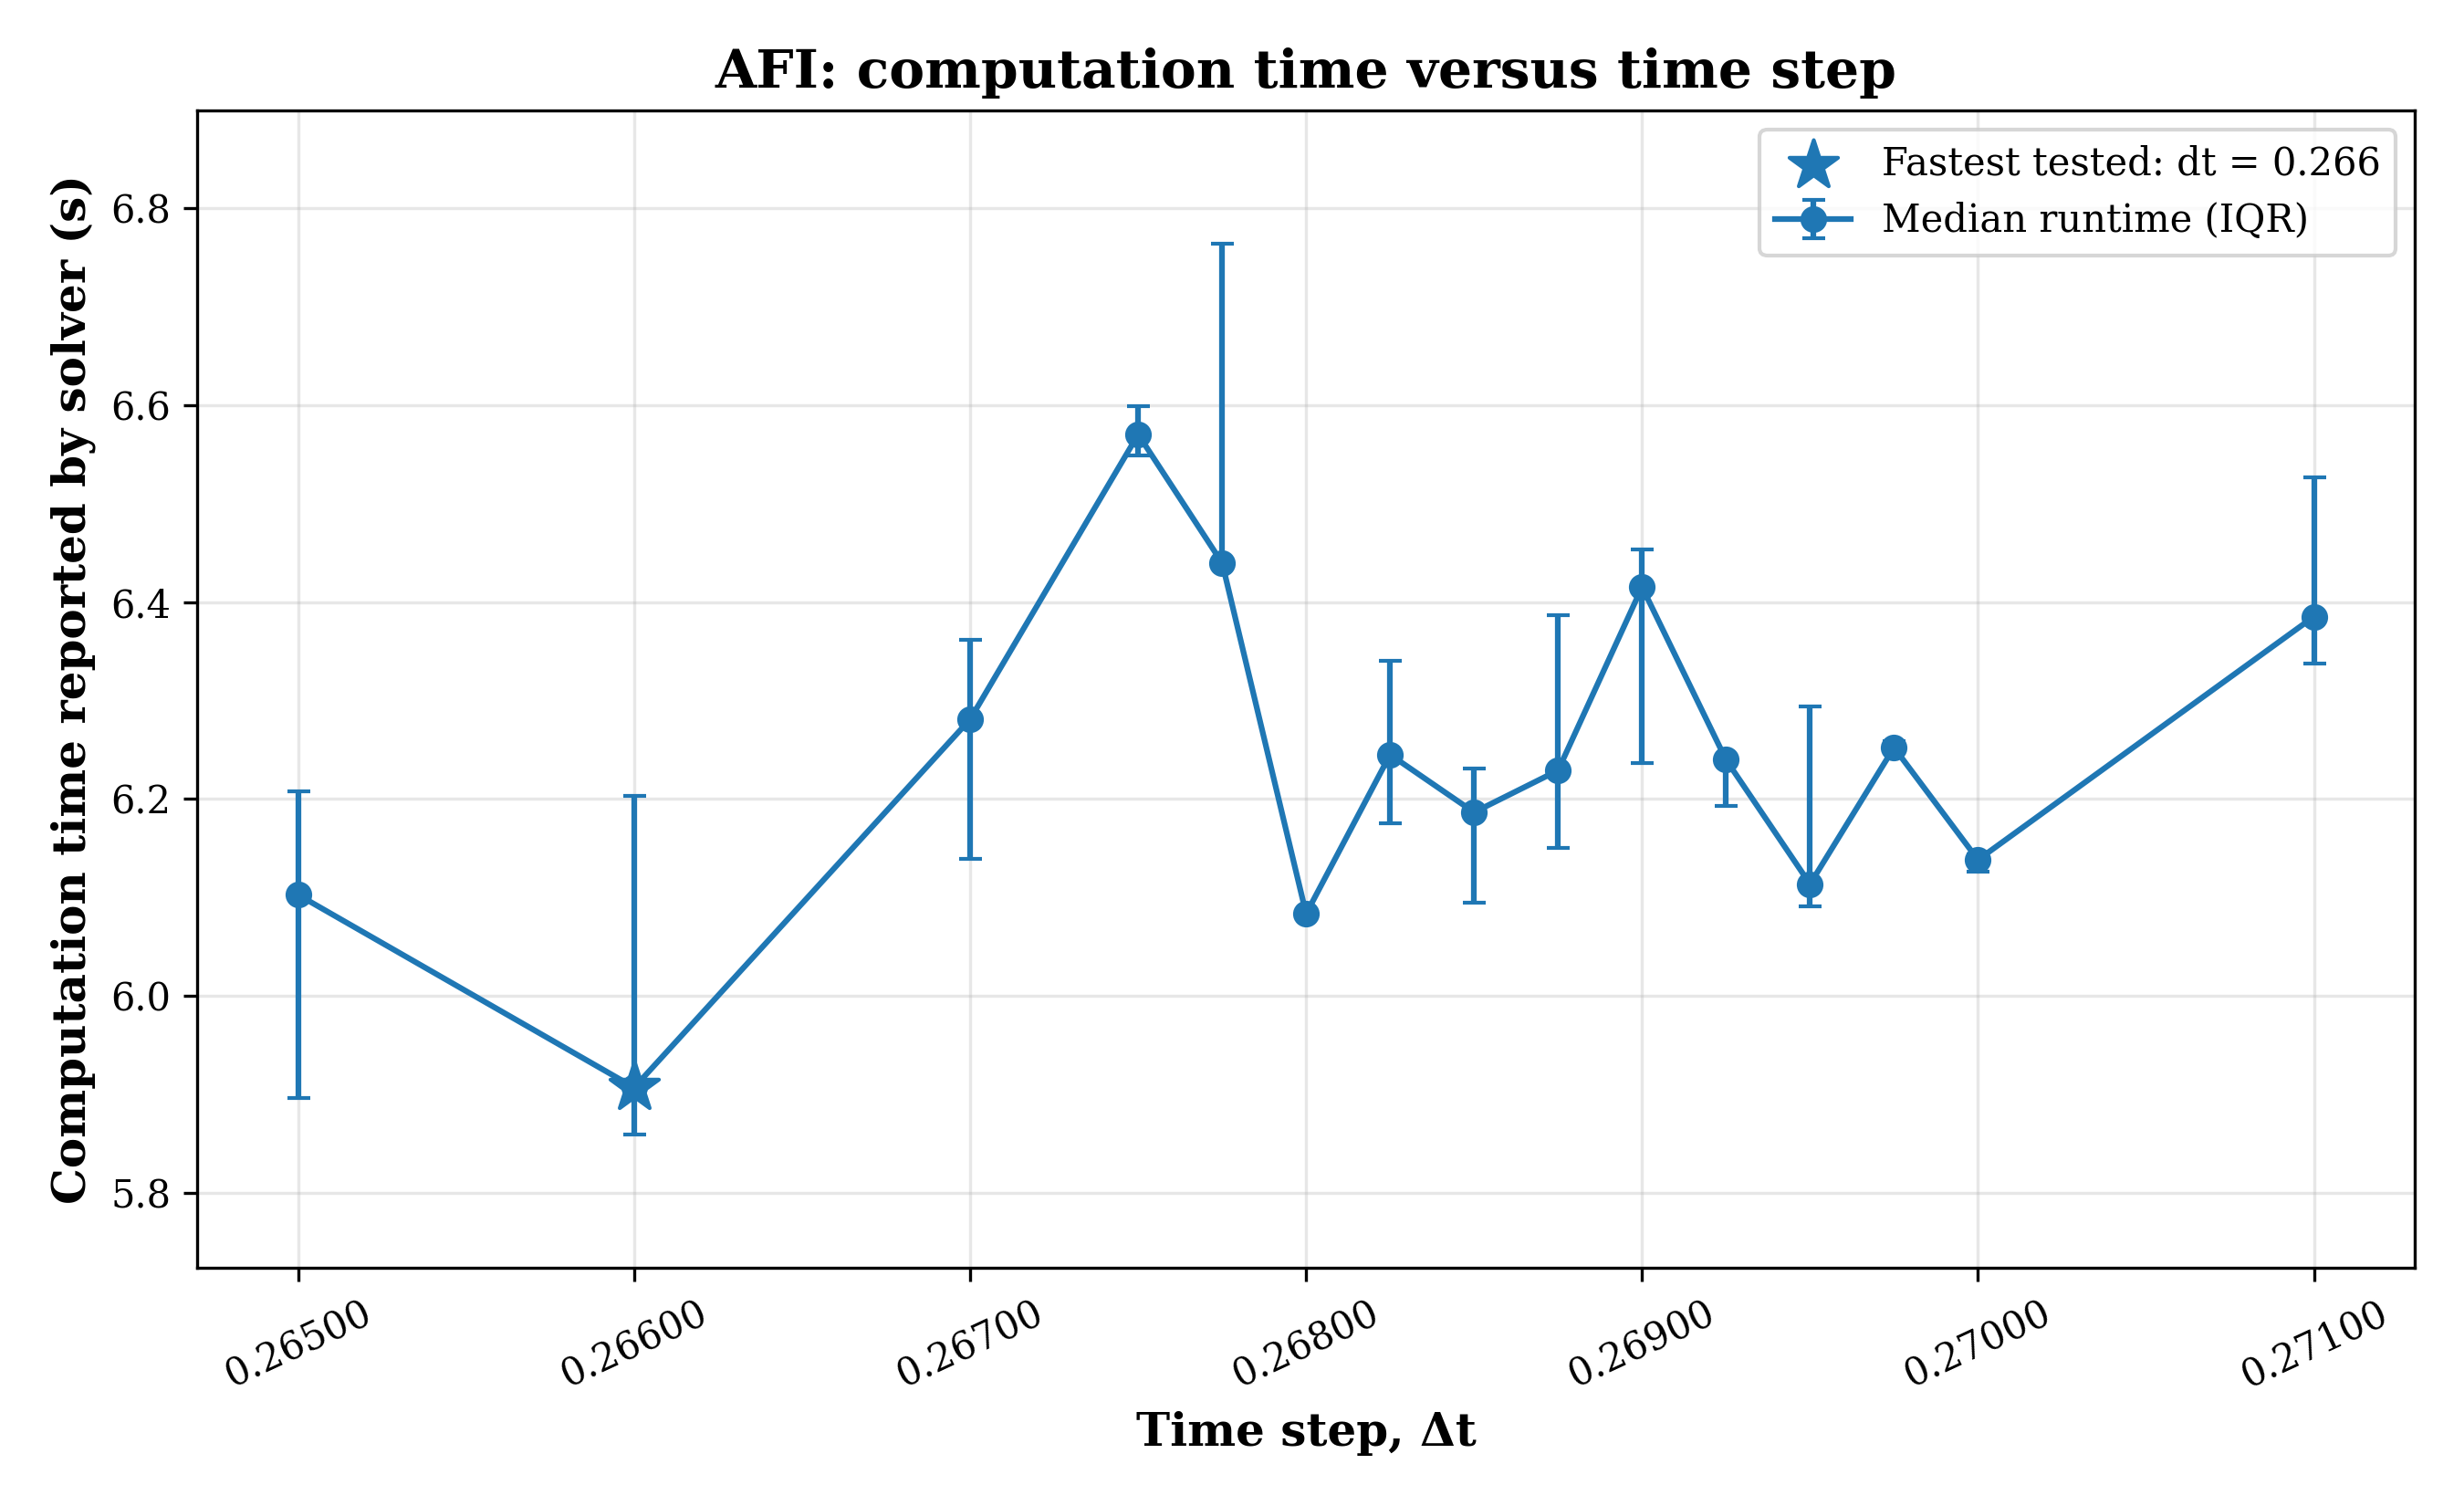
\includegraphics[width=0.85\textwidth]
    {figures/runtime_vs_dt_AFI.png}
    \caption{Median computation time of AFI as a function
    of the pseudo-time step. The minimum among the tested
    values occurs at $\Delta t=0.266$.}
    \label{fig:afi_timestep_efficiency}
\end{figure}

For the direct implicit solver, the representative value
$\Delta t=1$ was selected instead of the very large
time step that produced the minimum runtime in the
preliminary sweep. The preliminary sweep identified
$\Delta t=20000$ as its fastest tested case, but this
extremely aggressive pseudo-time step was not retained
for the comparison. The direct solver must therefore be
rerun at $\Delta t=1$ to determine its median computation
time, iteration count, and final residual. These results
will be used to assess its practical efficiency alongside
AFI under the selected settings.

\subsubsection{Comparison of the Converged Solutions}

To verify that the two solvers produce the same
steady-state solution, their temperature fields at the
selected time steps should be compared over the physical
cells, excluding ghost cells. The relative $L_2$ difference
is defined as
\begin{equation}
    \varepsilon_{\mathrm{AFI,Direct}}
    =
    \frac{
    \left\|
    \mathbf{T}_{\mathrm{AFI}}
    -
    \mathbf{T}_{\mathrm{Direct}}
    \right\|_2
    }{
    \left\|
    \mathbf{T}_{\mathrm{Direct}}
    \right\|_2
    }.
    \label{eq:afi_direct_relative_difference}
\end{equation}
This quantity should be recalculated using the direct
solution obtained with $\Delta t=1$. The previously
obtained value of $1.15\times10^{-14}$ corresponds to
the direct-solver run at $\Delta t=20000$ and is therefore
not reported as the result of the revised comparison.

The computation-time comparison should likewise use the
new direct-solver measurement at $\Delta t=1$. Since the
direct solver's runtime and iteration count can change
with the selected time step, no speedup ratio is reported
until the revised run has been completed. Any resulting
performance comparison remains specific to the present
grid, problem configuration, and implementation.

\subsection{Comparison of Solver Performance}

The computational performance of the four numerical methods
was compared using the selected pseudo-time steps:
$\Delta t=0.265$ for AFI, $\Delta t=1$ for the direct
implicit solver, $\Delta t=0.017$ for RK2, and
$\Delta t=0.024$ for RK4. These values were selected based
on the preceding time-step and stability analyses. The
explicit methods use time steps slightly below their
estimated stability limits, while the direct solver uses
a representative time step of $1$ rather than an
excessively large value.

All simulations were performed on the same $50\times20$
grid with $\mathrm{Pe}=17.5$, $\mathrm{Br}=0.2$, and a
convection coefficient of $1$. Five independent runs
were performed for each method, with the initial
temperature field reconstructed before every run. The
convergence criterion was a steady-state residual
tolerance of $10^{-12}$. The elapsed wall-clock time was
measured around each solver call, including solver-specific
setup operations such as matrix assembly and factorization.
The construction of the initial temperature and velocity
fields and the independent residual evaluation were
excluded from the measured time.

Table~\ref{tab:solver_comparison} summarizes the results.
All five runs of each method converged to the prescribed
residual tolerance. The reported computation times are
the medians of the five runs, and the standard deviations
indicate the variation in runtime.

\begin{table}[htbp]
    \centering
    \small
    \caption{Performance comparison of the four numerical
    methods on the $50\times20$ grid.}
    \label{tab:solver_comparison}
    \begin{tabular}{@{}l c c c c c@{}}
        \hline
        Method
        & $\Delta t$
        & Iterations
        & Median time (s)
        & Std. dev. (s)
        & Final residual
        \\
        \hline
        AFI
        & $0.265$
        & $295$
        & $6.2817$
        & $0.1800$
        & $9.398\times10^{-13}$
        \\[0.1cm]
        Direct implicit Euler
        & $1.0$
        & $16$
        & $0.1403$
        & $0.0094$
        & $6.322\times10^{-13}$
        \\[0.1cm]
        Explicit RK2
        & $0.017$
        & $392$
        & $8.0148$
        & $0.1089$
        & $9.907\times10^{-13}$
        \\[0.1cm]
        Explicit RK4
        & $0.024$
        & $309$
        & $10.7187$
        & $0.1100$
        & $9.748\times10^{-13}$
        \\
        \hline
    \end{tabular}
\end{table}

In addition to the final performance measurements, the
convergence histories were examined to compare the
behavior of the methods throughout the iterations.
Figures~\ref{fig:residual_vs_iteration} and
\ref{fig:residual_vs_time} show the steady-state residual
as a function of iteration number and elapsed computation
time, respectively. For each method, the plotted history
corresponds to the successful run whose total runtime was
closest to the median runtime of its five runs. This
provides a representative convergence history for each
method without superimposing all five runs.

\begin{figure}[htbp]
    \centering
    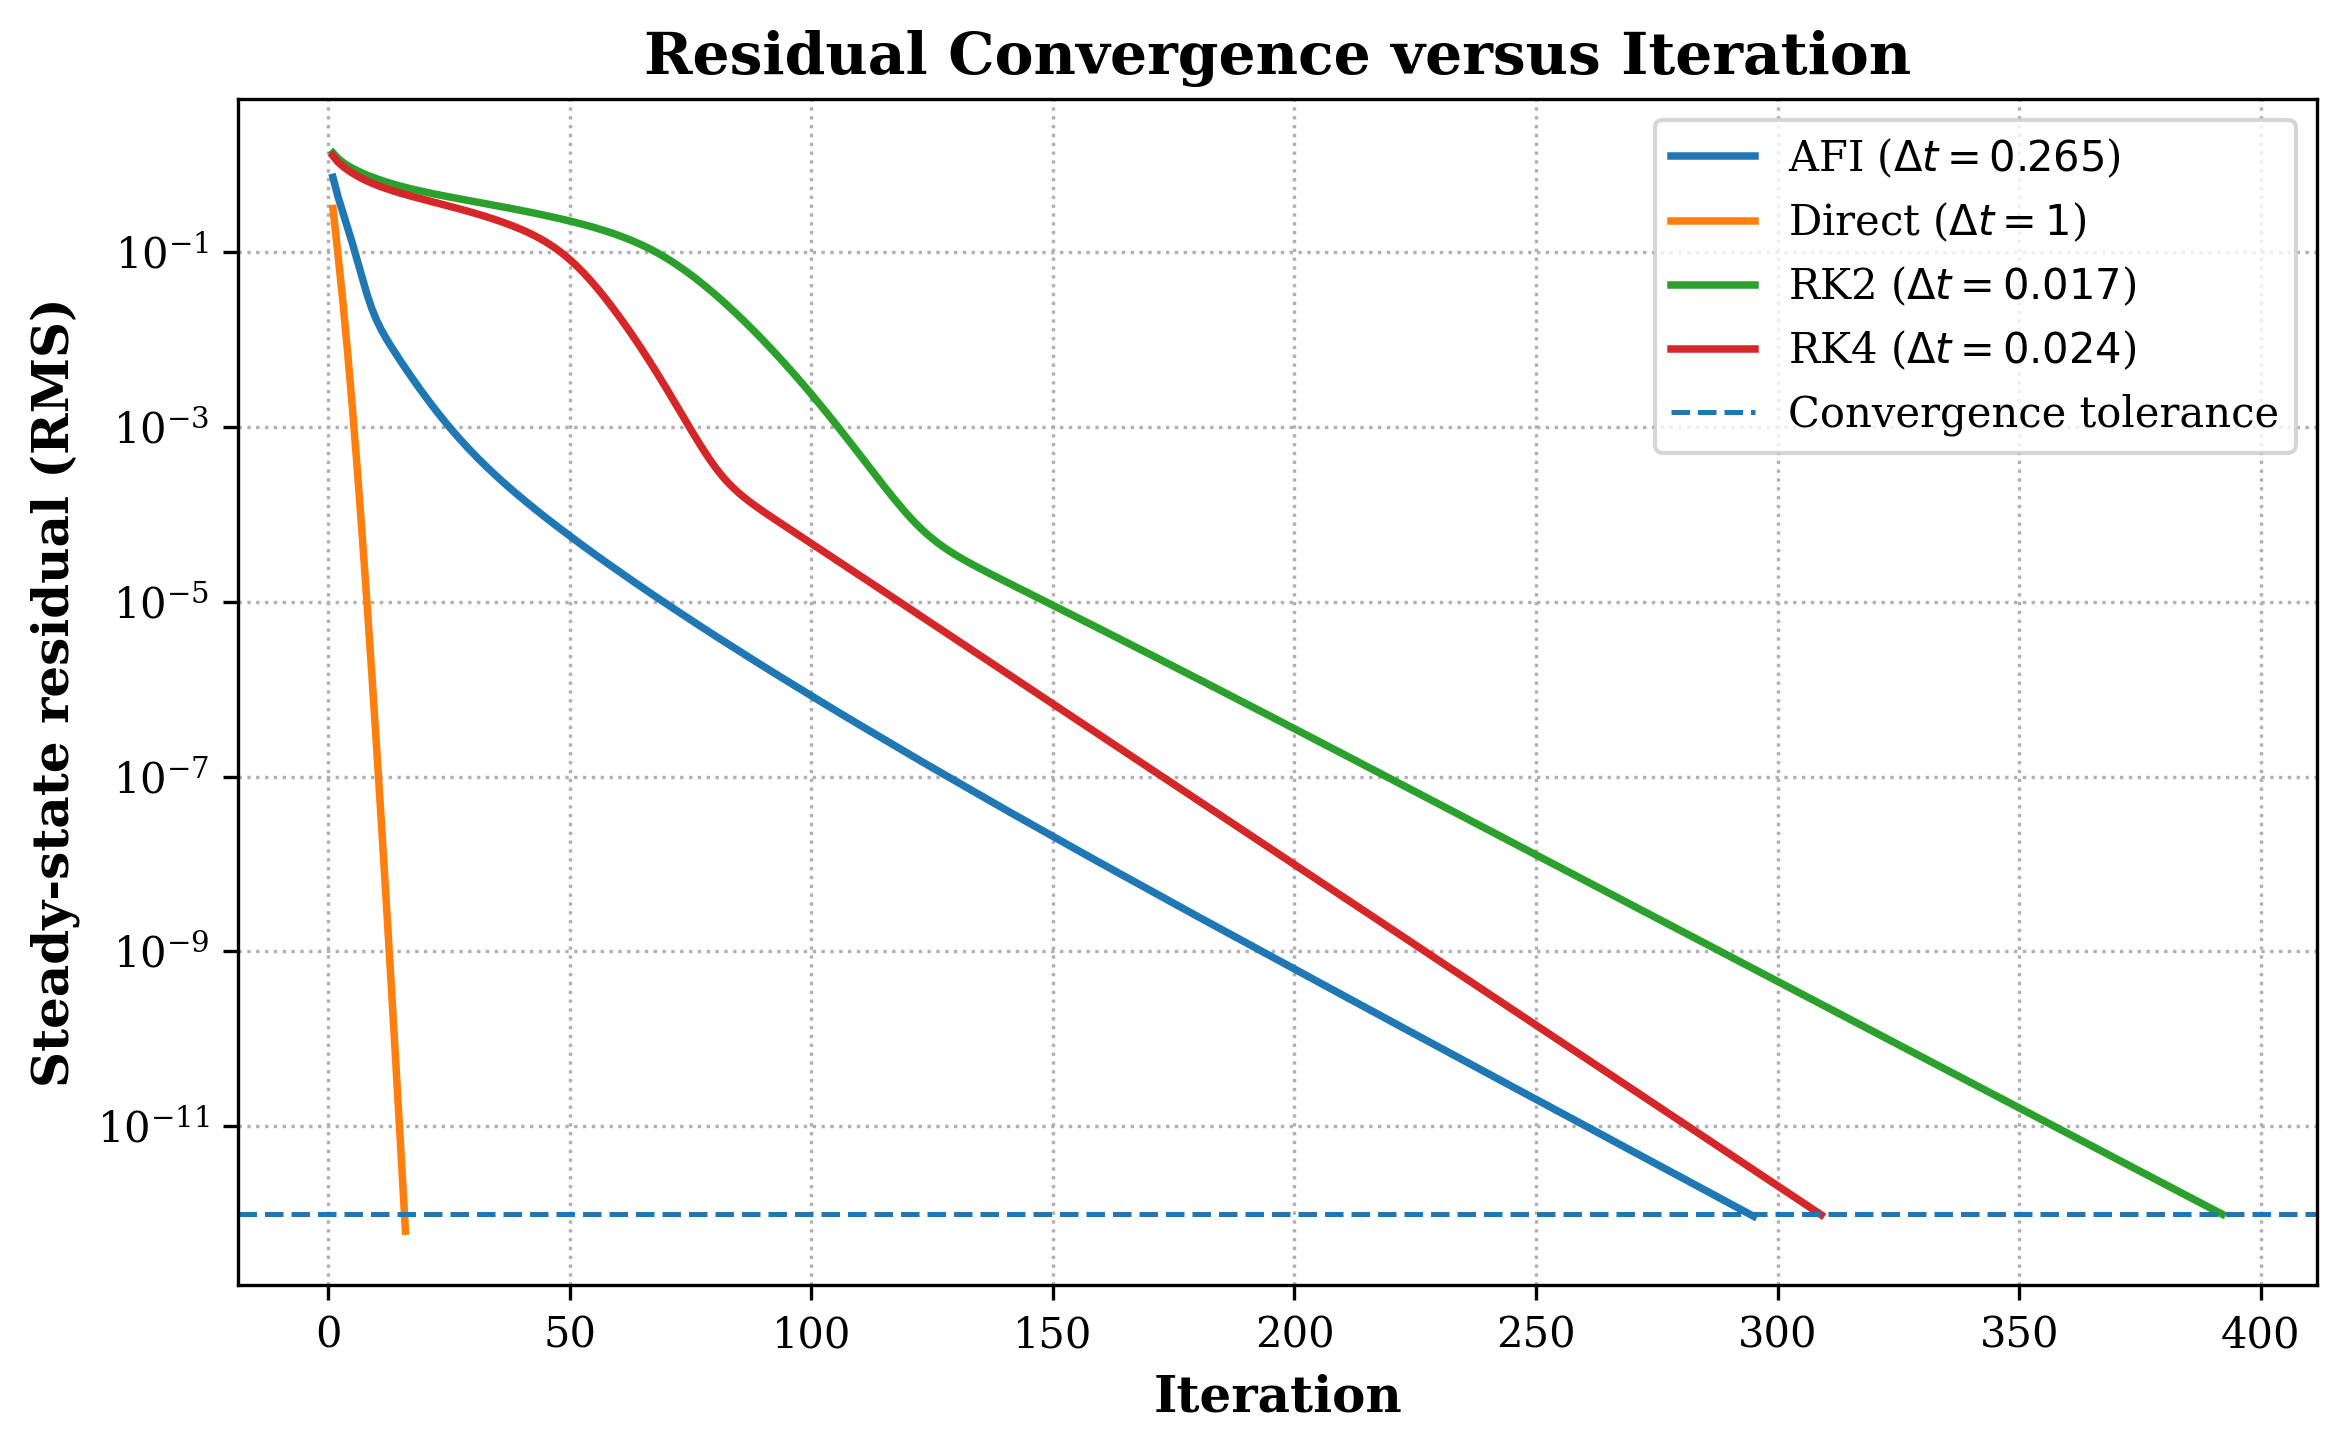
\includegraphics[width=0.85\textwidth]
    {figures/residual_vs_iteration.png}
    \caption{Steady-state residual versus iteration number
    for the four numerical methods. The dashed line
    indicates the convergence tolerance of $10^{-12}$.}
    \label{fig:residual_vs_iteration}
\end{figure}

Figure~\ref{fig:residual_vs_iteration} compares the
convergence behavior in terms of iteration count. The
direct implicit solver reached the prescribed tolerance
in only 16 iterations, compared with 295 for AFI, 392
for RK2, and 309 for RK4. RK4 required fewer iterations
than RK2, while the direct method converged in
substantially fewer iterations than the other methods.

\begin{figure}[htbp]
    \centering
    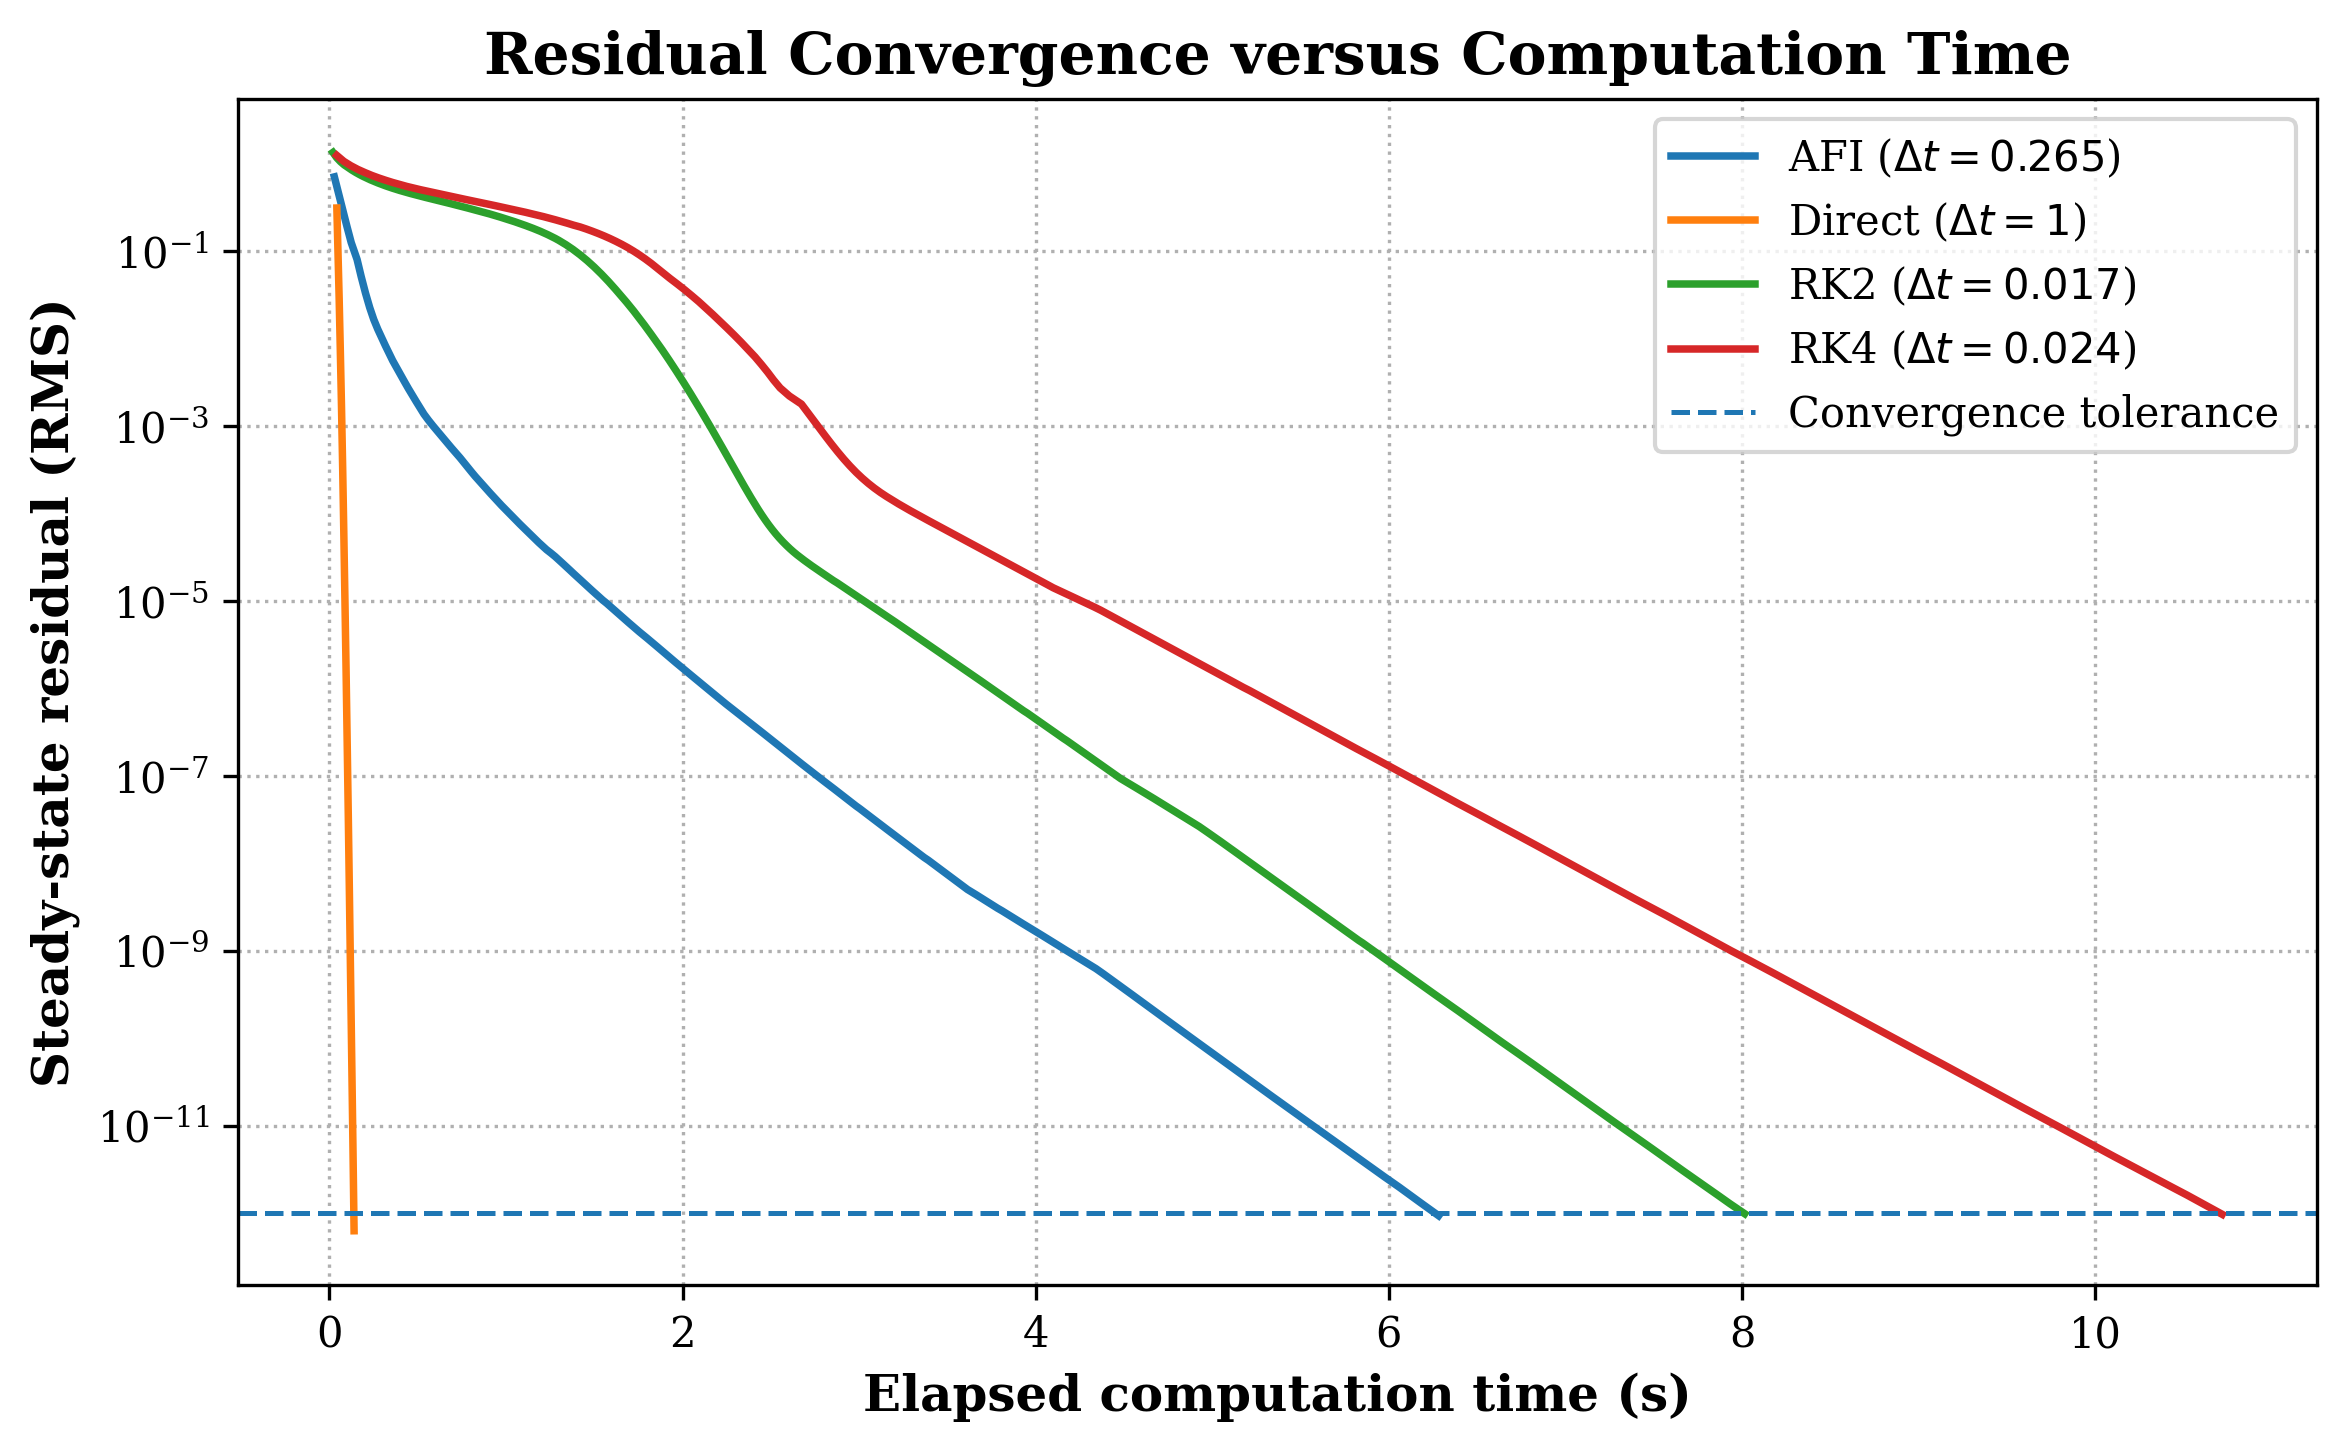
\includegraphics[width=0.85\textwidth]
    {figures/residual_vs_time.png}
    \caption{Steady-state residual versus elapsed
    computation time for the four numerical methods.
    The dashed line indicates the convergence tolerance
    of $10^{-12}$.}
    \label{fig:residual_vs_time}
\end{figure}

The residual-versus-time histories provide a direct
comparison of the computational effort required to
reach the prescribed convergence tolerance. The direct
implicit solver achieved the lowest median computation
time, at $0.1403~\mathrm{s}$. Relative to this method,
AFI, RK2, and RK4 required approximately 44.8, 57.1,
and 76.4 times more computation time, respectively.
Although RK4 required fewer iterations than RK2, its
overall computation time was higher. This is consistent
with the greater computational cost of its four-stage
time-integration procedure compared with the two-stage
RK2 method.

AFI was faster than both explicit Runge--Kutta methods
for the selected time steps, despite requiring more
iterations than RK4 and fewer than RK2. This indicates
that iteration count alone does not determine the
computational cost; the operations required within each
iteration also influence the total runtime.

All four methods satisfied the same steady-state
residual criterion in all five runs. The direct implicit
solver was the most computationally efficient among
the tested methods. However, these runtime ratios apply
specifically to the present grid, implementation, and
selected time steps. They should not be interpreted as
general performance rankings for other grid sizes or
problem configurations.


\subsection{Pseudo-Time Evolution of the Temperature Field}
\label{subsec:temperature_evolution}

The development of the temperature field during the numerical
solution is illustrated in Figure~\ref{fig:final_temperature}.
The sequence of temperature distributions shows the combined
effects of convection, thermal diffusion, and viscous
dissipation as the solution evolves from the initial condition
toward the steady state.

The effect of convection is evident from the deformation
of the temperature contours along the channel. Since the
prescribed parabolic velocity profile varies across the
channel height, fluid near the centreline is transported
downstream faster than fluid near the walls. This produces
a curved, approximately hyperbolic pattern in the
temperature distribution.

Viscous dissipation introduces a symmetric heating
contribution across the channel. This follows from the
squared wall-normal velocity gradient, which is symmetric
about the channel centreline and reaches its maximum
magnitude near the two walls. Consequently, the temperature
in the fluid cells adjacent to the lower wall initially
increases due to viscous heating. As the solution develops,
this local temperature increase is followed by a slight
decrease, as convective transport of relatively cooler
fluid from the inlet competes with the heating contribution.

The effect of thermal diffusion is particularly visible
in the downstream region of the channel. Heat is conducted
in the wall-normal direction from the warmer upper region
toward the cooler lower region, leading to a gradual
redistribution and smoothing of the temperature field
across the channel height.

Overall, the temperature evolution illustrates the
interaction between the three transport mechanisms and
their contributions to the resulting steady-state
temperature distribution.

\begin{figure}[htbp]
    \centering
    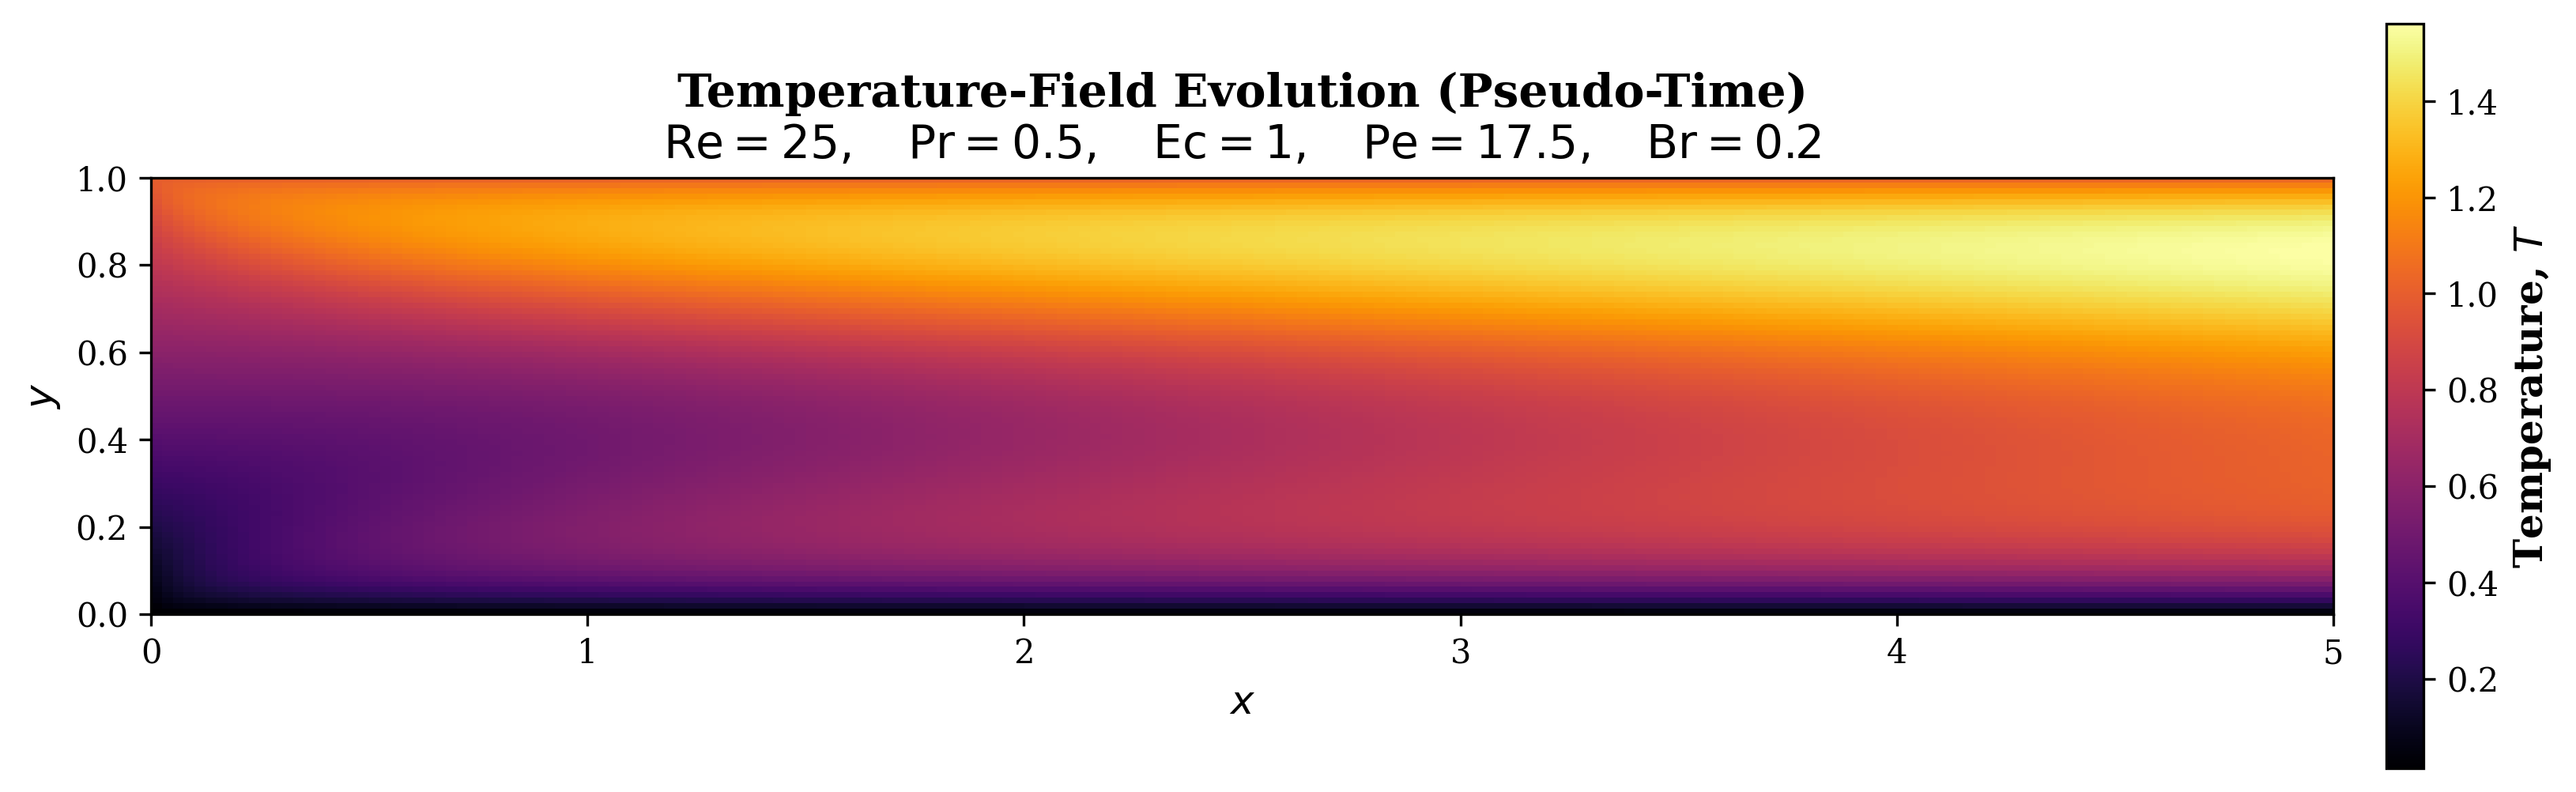
\includegraphics[width=0.85\textwidth]
    {figures/final_temperature.png}
    \caption{Representative temperature-field distribution
    during pseudo-time integration.}
    \label{fig:final_temperature}

    \vspace{0.2cm}
    \small
    \href{run:figures/temperature_evolution.gif}
    {Click here to view the complete temperature evolution
    animation (gif).}
\end{figure}

\subsection{Parameter Study}

A parameter study was conducted to examine the effects of viscous dissipation,
convection strength, and the Peclet number on the steady-state temperature
distribution. All cases were solved on a $100\times40$ mesh using the APF
solver, with a pseudo-time step of $\Delta t=0.05$ and a convergence
tolerance of $10^{-10}$. The initial temperature and inlet temperature
profiles were both prescribed as $T=y$.

\subsubsection{Effect of the Brinkman Number}

The Brinkman number controls the strength of viscous dissipation relative
to thermal diffusion. Three cases were considered, with
$Br=0$, $0.07$, and $0.2$, while the Peclet number and convection
coefficient were kept fixed at $Pe=17.5$ and $\gamma_c=1$.

For $Br=0$, the temperature field remains close to the initial linear
distribution. This behaviour is consistent with the prescribed boundary
conditions: the initial and inlet profiles are both $T=y$, and the
temperature distribution satisfies the wall temperatures. In the absence
of viscous dissipation, this profile is also a steady solution of the
energy equation.

As the Brinkman number increases, viscous heating produces a progressively
larger departure from the initial linear distribution. Since the
dissipation source is proportional to the square of the velocity gradient,
its contribution is strongest near the channel walls, where the velocity
gradient is largest. The upper part of the channel reaches higher
temperatures due to the combined effects of viscous heating and the
prescribed higher temperature at the upper wall.

Figure~\ref{fig:brinkman_study} compares the resulting temperature fields
for the three Brinkman numbers. All contours use the same temperature
scale to facilitate comparison.

\begin{figure}[htbp]
    \centering
    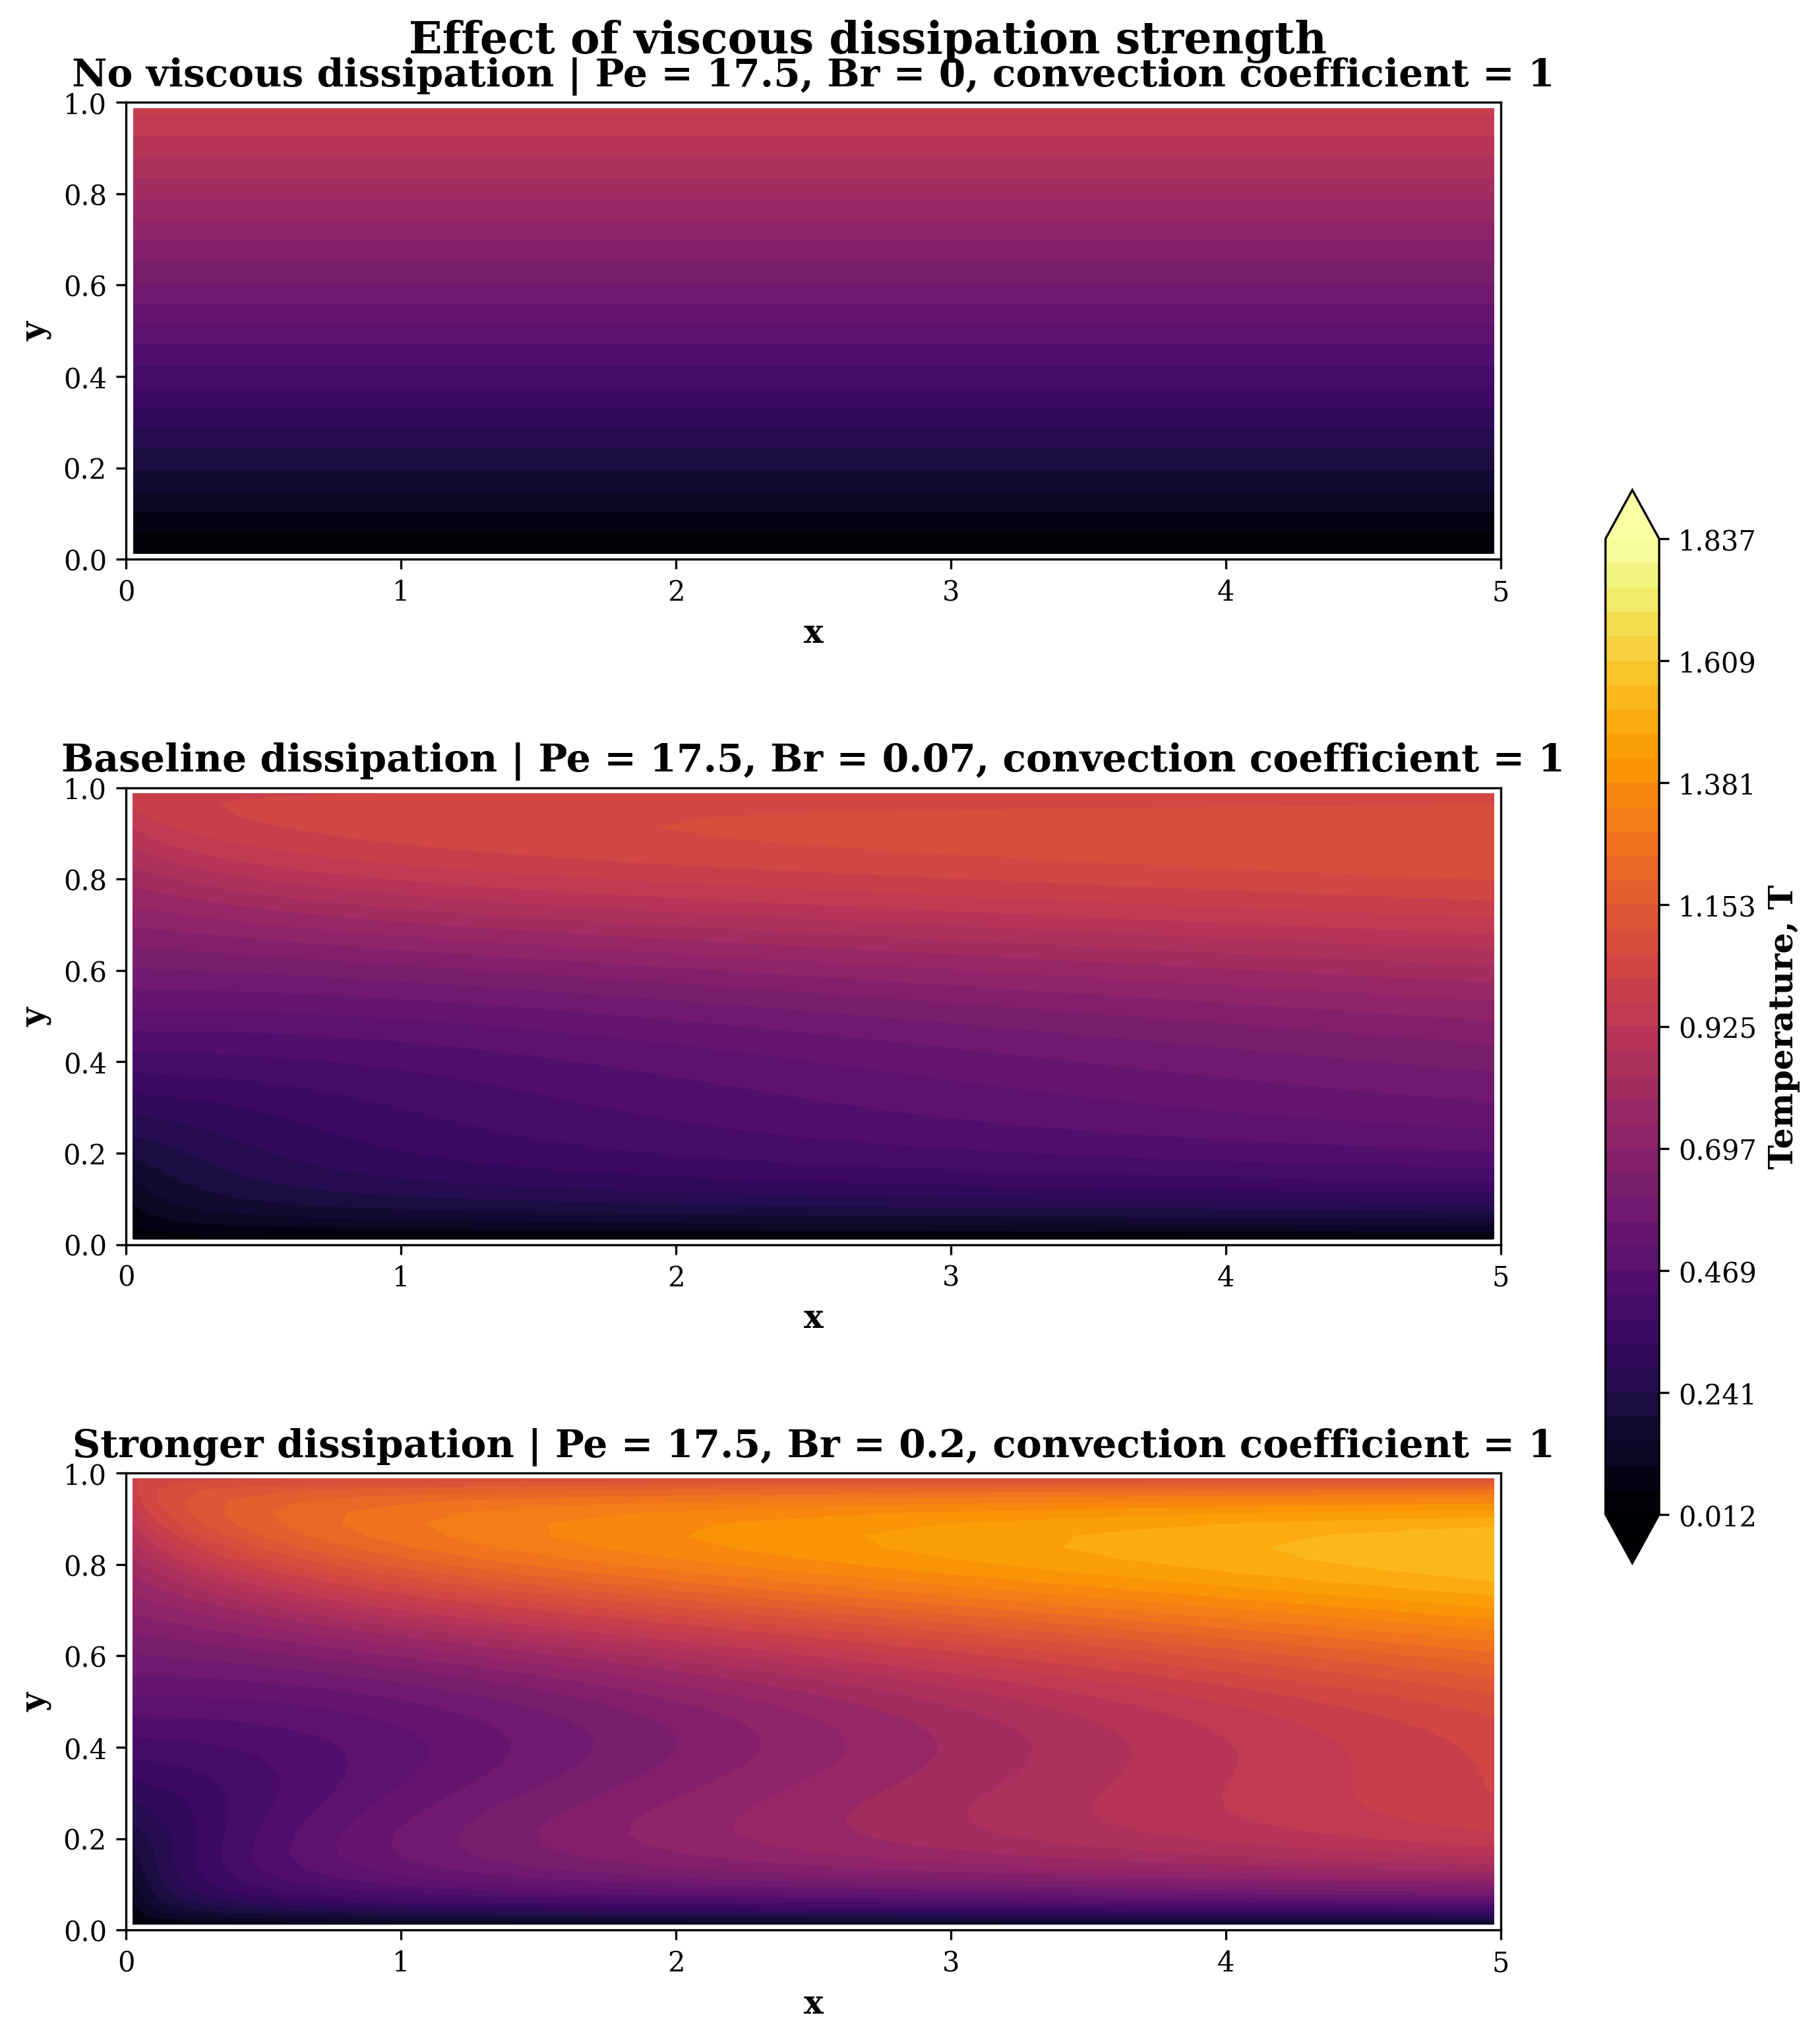
\includegraphics[width=0.88\textwidth]
    {figures/brinkman_number.png}
    \caption{Effect of the Brinkman number on the steady-state temperature
    distribution for $Pe=17.5$ and $\gamma_c=1$.}
    \label{fig:brinkman_study}
\end{figure}


\subsubsection{Effect of the Convection Coefficient}

The convection coefficient $\gamma_c$ scales the convective contribution
in the energy equation. Its effect was examined using
$\gamma_c=0.4$, $1$, and $10$, while keeping $Pe=17.5$ and $Br=0.2$
constant.

For a large convection coefficient, the temperature field remains closer
to the imposed inlet profile. This is expected because stronger convection
transports the inlet temperature distribution downstream and limits the
relative influence of thermal diffusion and viscous heating.

Reducing the convection coefficient weakens this transport. Consequently,
thermal diffusion and viscous dissipation have a greater influence on
the temperature field. The resulting distribution departs further from
the initial linear profile, with a more pronounced temperature increase
in the upper region of the channel.

The three cases are compared in Figure~\ref{fig:convection_study}.
The differences illustrate how the relative strengths of convection,
thermal diffusion, and viscous heating determine the resulting
temperature distribution.

\begin{figure}[htbp]
    \centering
    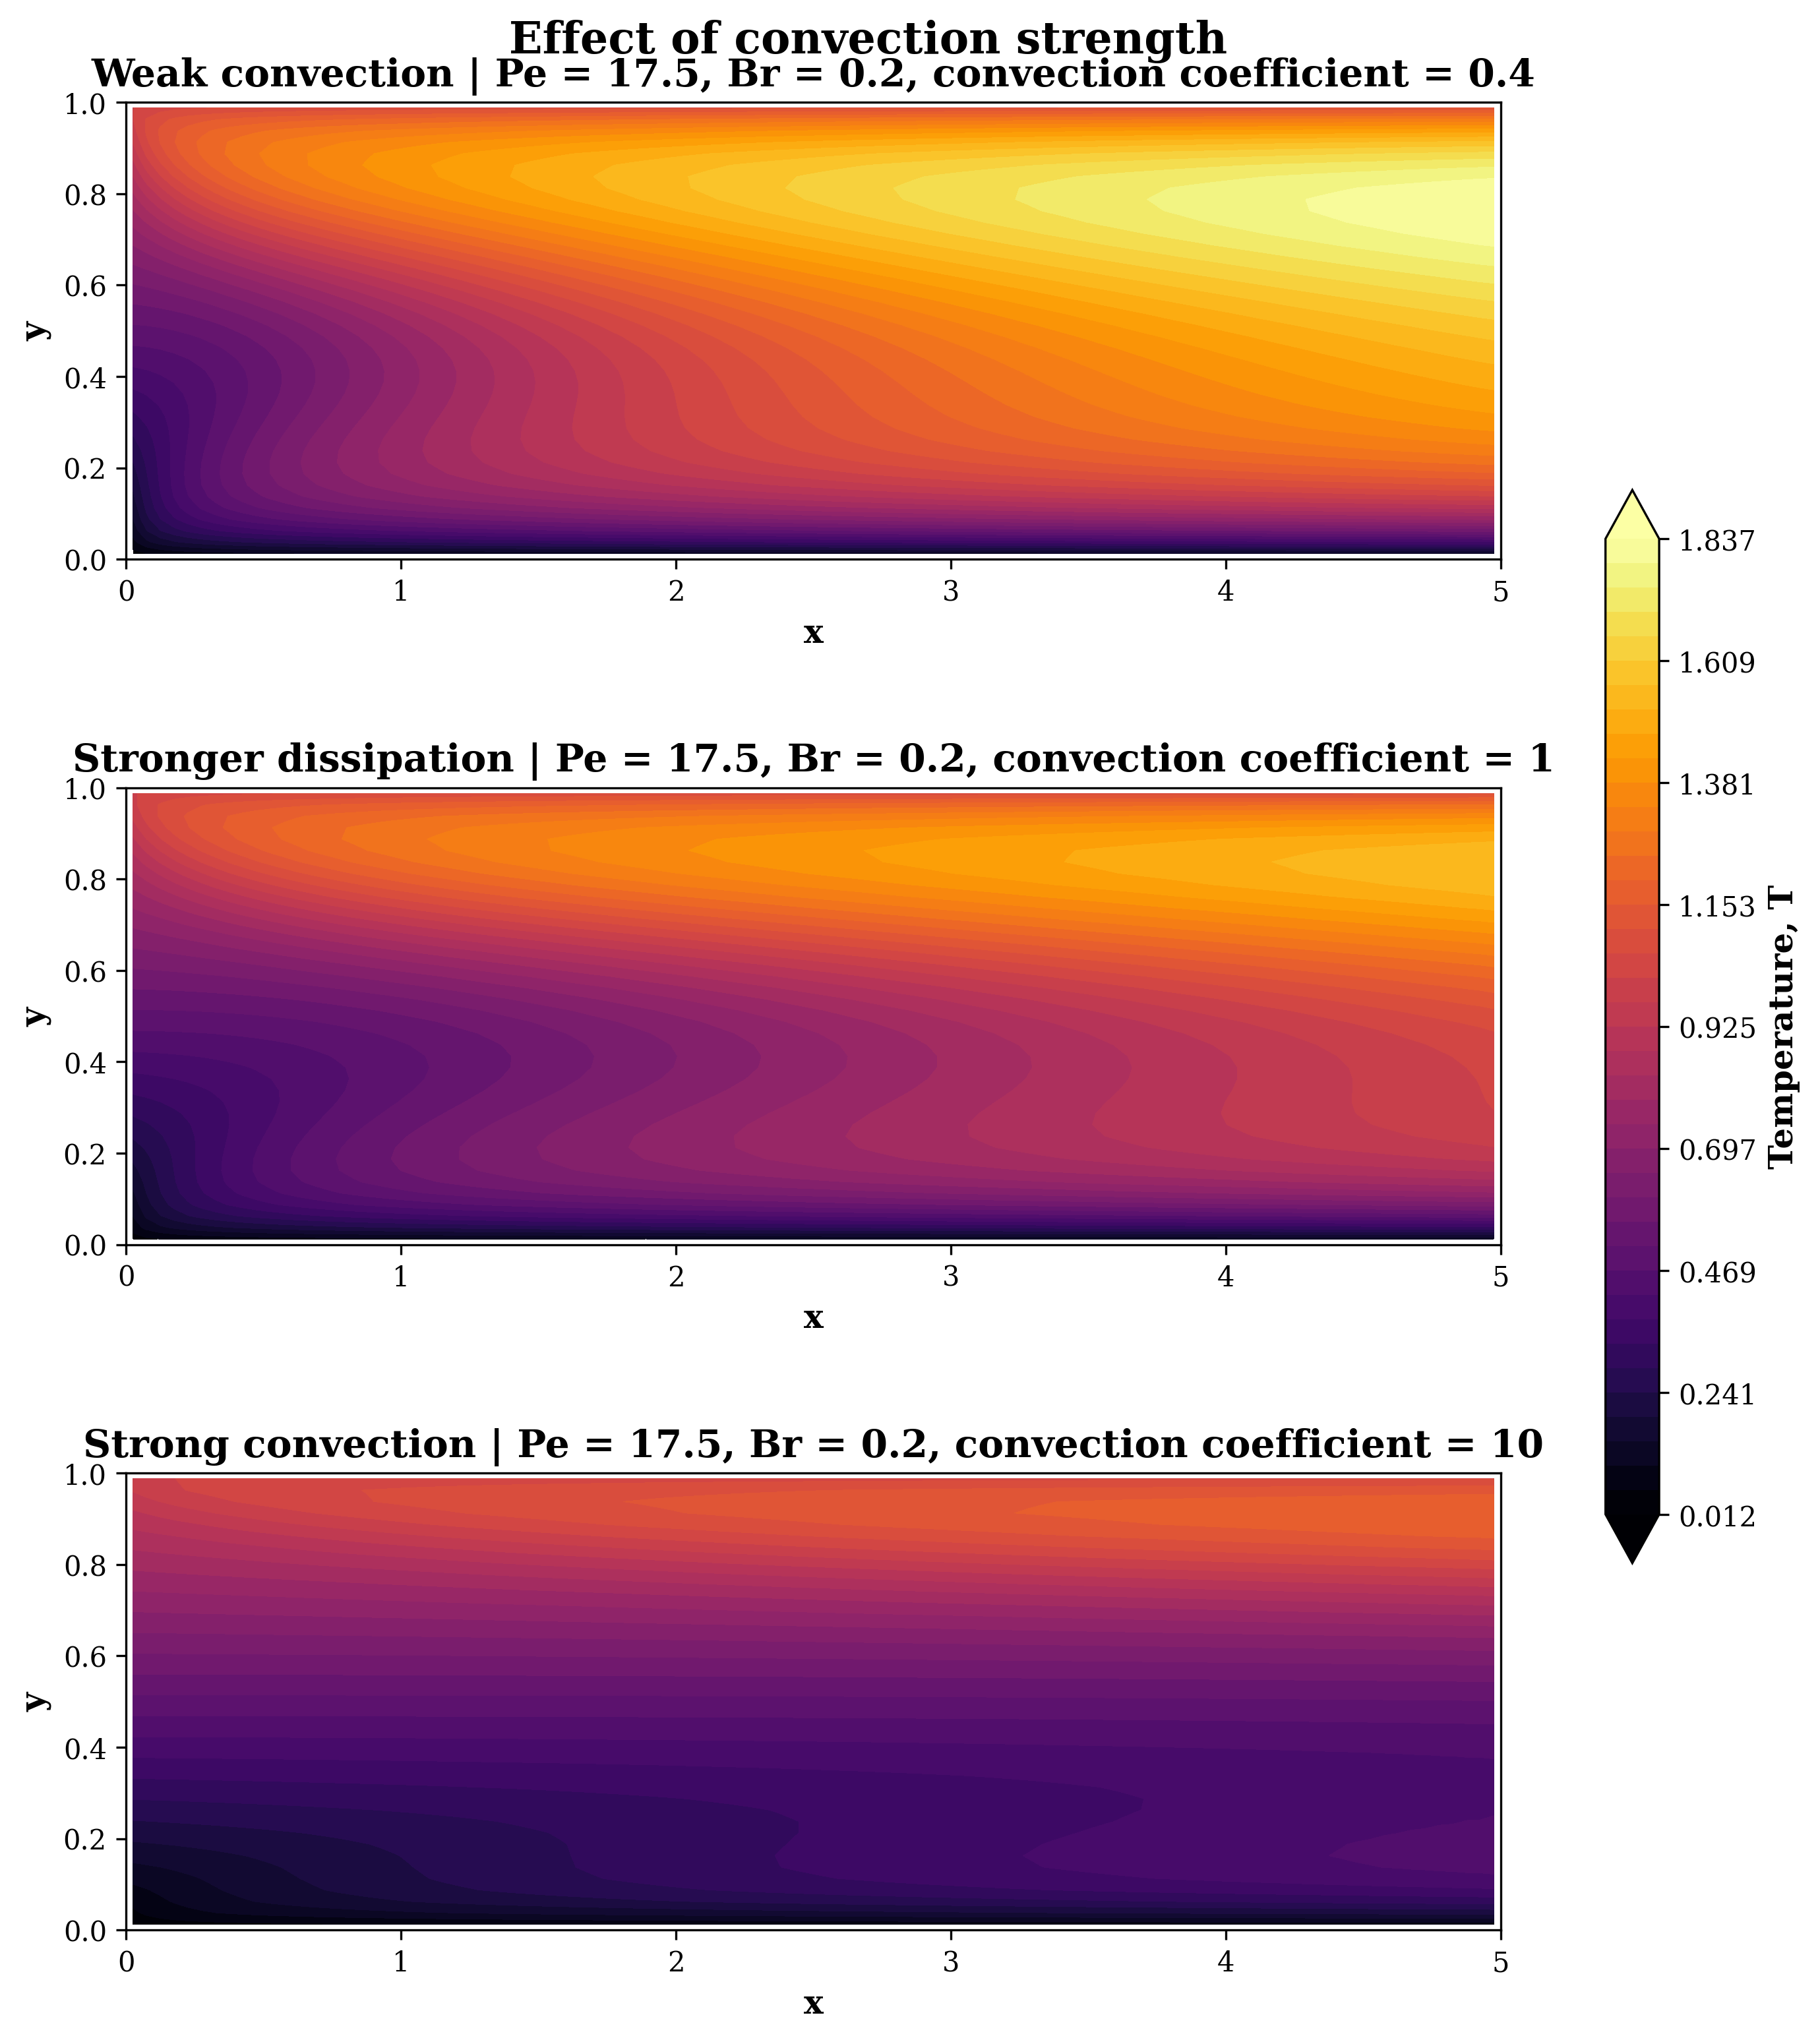
\includegraphics[width=0.88\textwidth]
    {figures/convection_coefficient.png}
    \caption{Effect of the convection coefficient on the steady-state
    temperature distribution for $Pe=17.5$ and $Br=0.2$.}
    \label{fig:convection_study}
\end{figure}


\subsubsection{Effect of the Peclet Number}

The Peclet number represents the relative strength of convective transport
to thermal diffusion. Its effect was studied at
$Pe=1$, $17.5$, and $50$. In these cases, the ratio $Br/Pe$ was held
constant at $0.004$, so the coefficient of the viscous dissipation source
remained unchanged.

A low Peclet number corresponds to stronger thermal diffusion relative
to convection. Since the initial and inlet temperature profiles are
identical, the temperature field tends to remain close to the linear
distribution. Thermal diffusion also smooths temperature variations
produced by the viscous heating source.

As the Peclet number increases, the relative influence of thermal
diffusion decreases. The temperature field therefore exhibits a greater
departure from the initial profile under the combined effects of
convection and viscous dissipation. In particular, the temperature
variations generated by the dissipation source are less strongly
smoothed by diffusion.

Figure~\ref{fig:peclet_study} compares the temperature fields at the
three Peclet numbers. The results demonstrate the influence of thermal
diffusion on the balance between convective transport and viscous
heating.

\begin{figure}[htbp]
    \centering
    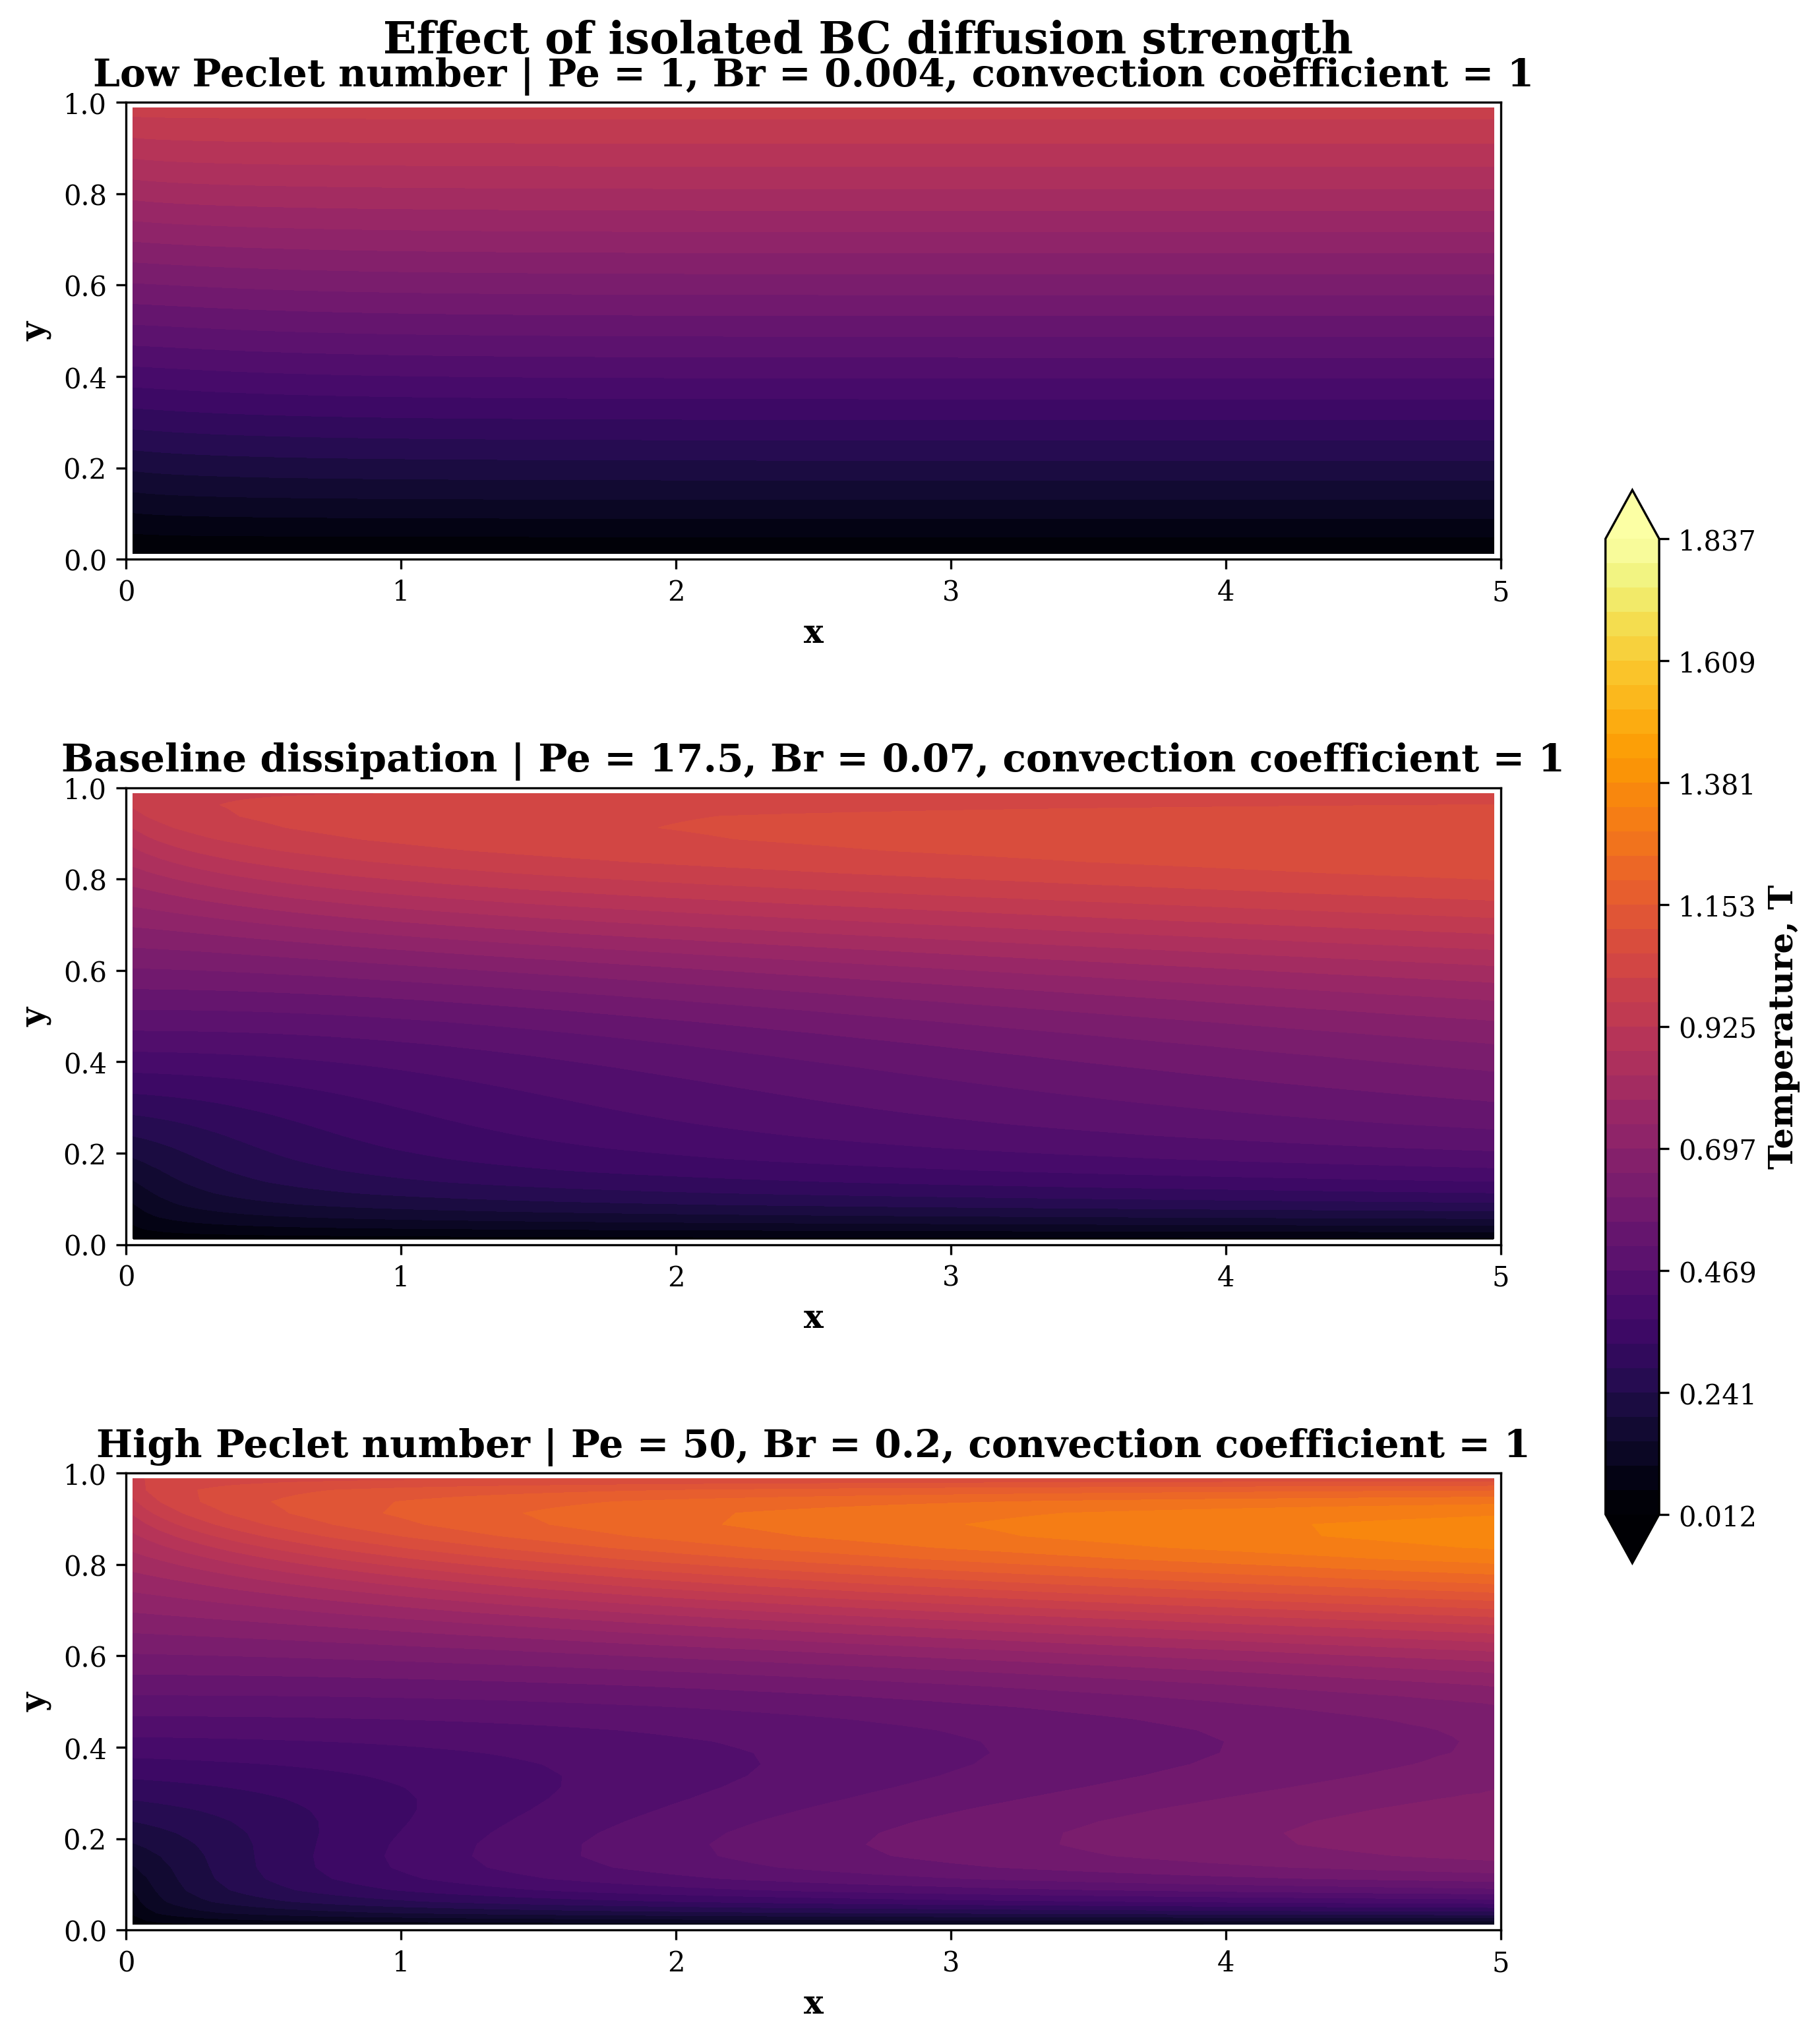
\includegraphics[width=0.88\textwidth]
    {figures/peclet_number.png}
    \caption{Effect of the Peclet number on the steady-state temperature
    distribution, with $Br/Pe=0.004$ and $\gamma_c=1$.}
    \label{fig:peclet_study}
\end{figure}


\subsubsection{Temperature Cross-Sections}

To examine the combined effects of convection and viscous dissipation
in more detail, temperature profiles were extracted at two streamwise
locations, $x/L_x=0.15$ and $0.85$. Three cases were selected for this
comparison:

\begin{itemize}
    \item Case 1: $Pe=17.5$, $Br=0.07$, and $\gamma_c=1$.
    \item Case 2: $Pe=17.5$, $Br=0.2$, and $\gamma_c=1$.
    \item Case 3: $Pe=17.5$, $Br=0.2$, and $\gamma_c=0.4$.
\end{itemize}

The first two cases have identical Peclet numbers and convection
coefficients. Their comparison therefore isolates the effect of
viscous dissipation. Increasing the Brinkman number from $0.07$ to
$0.2$ produces a more pronounced curvature in the wall-normal
temperature profiles. This reflects the stronger contribution of
viscous heating to the energy balance.

The second and third cases have the same Peclet and Brinkman numbers,
but different convection coefficients. Reducing $\gamma_c$ from
$1$ to $0.4$ weakens convective transport and increases the relative
influence of thermal diffusion and viscous heating. The resulting
profiles exhibit a warmer upper region and a less pronounced
wave-like variation, consistent with the smoothing effect of thermal
diffusion.

Together, these comparisons show that the temperature profiles result
from the combined effects of convective transport, thermal diffusion,
and viscous dissipation. Their relative contributions determine both
the temperature level and the shape of the wall-normal profiles.

\begin{figure}[htbp]
    \centering
    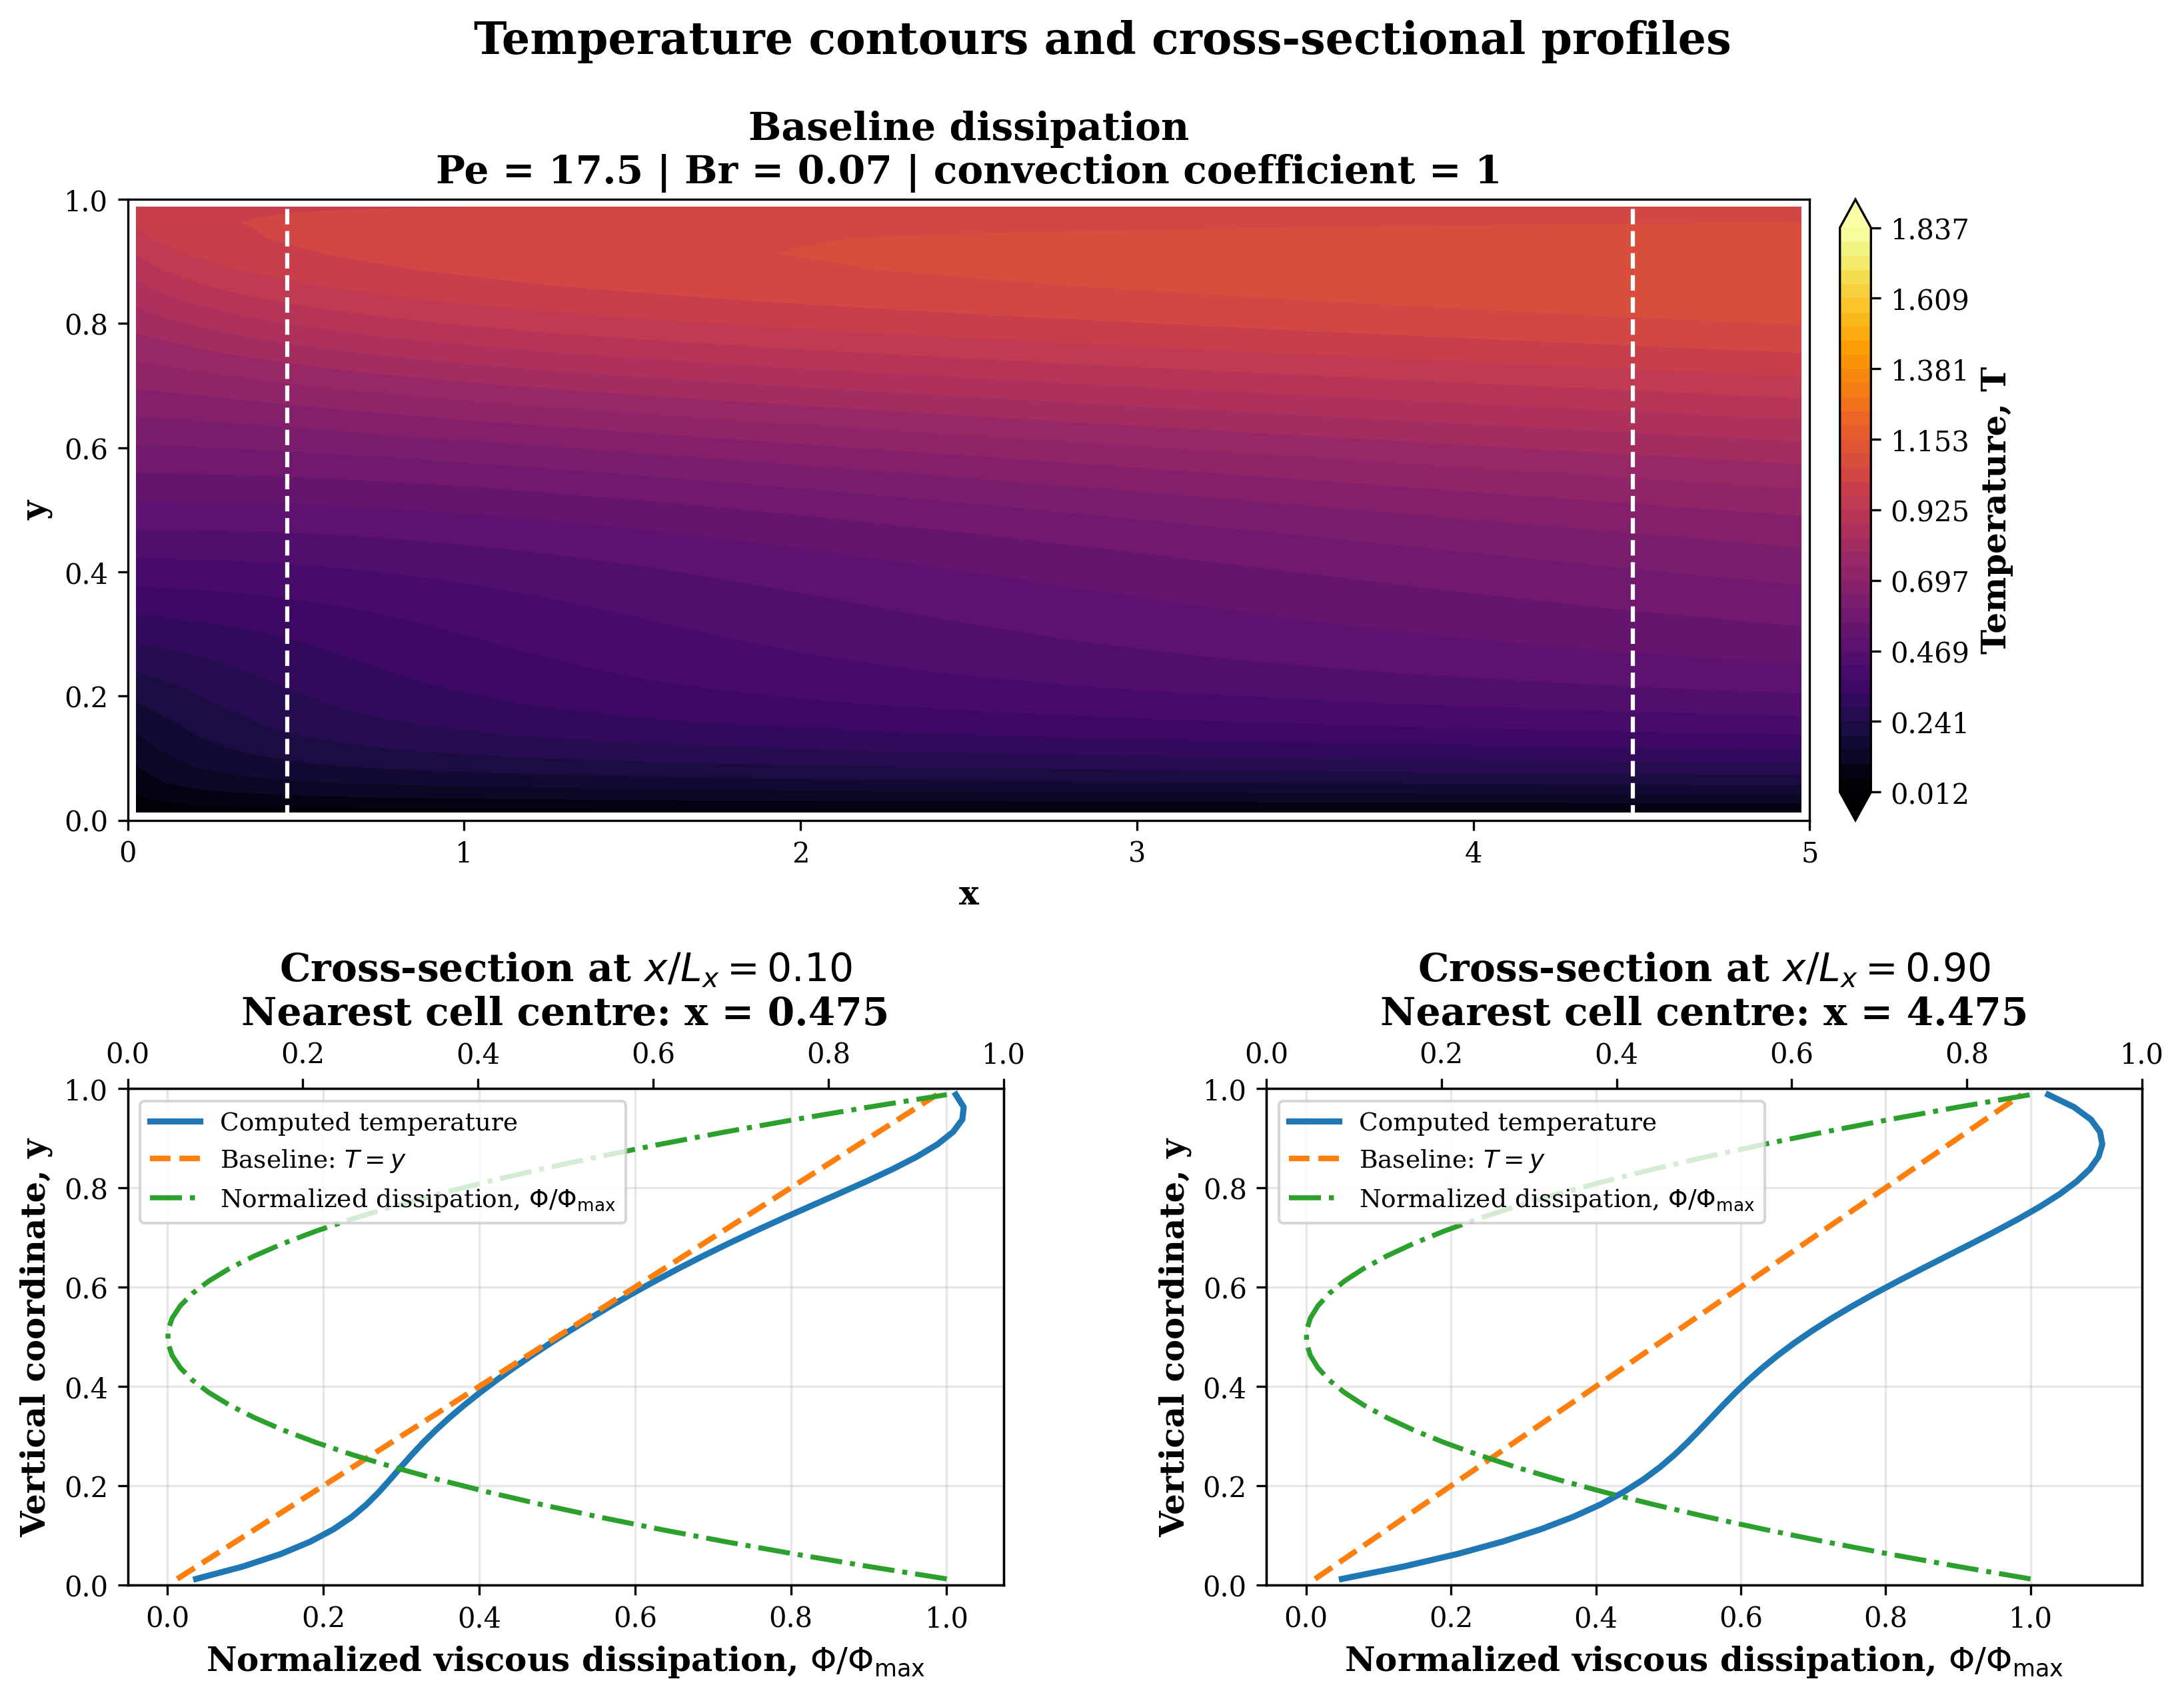
\includegraphics[width=0.88\textwidth]
    {figures/br_007_cross_sections.png}
    \caption{Temperature contours and wall-normal temperature profiles
    for $Pe=17.5$, $Br=0.07$, and $\gamma_c=1$.}
    \label{fig:cross_sections_br007}
\end{figure}

\begin{figure}[htbp]
    \centering
    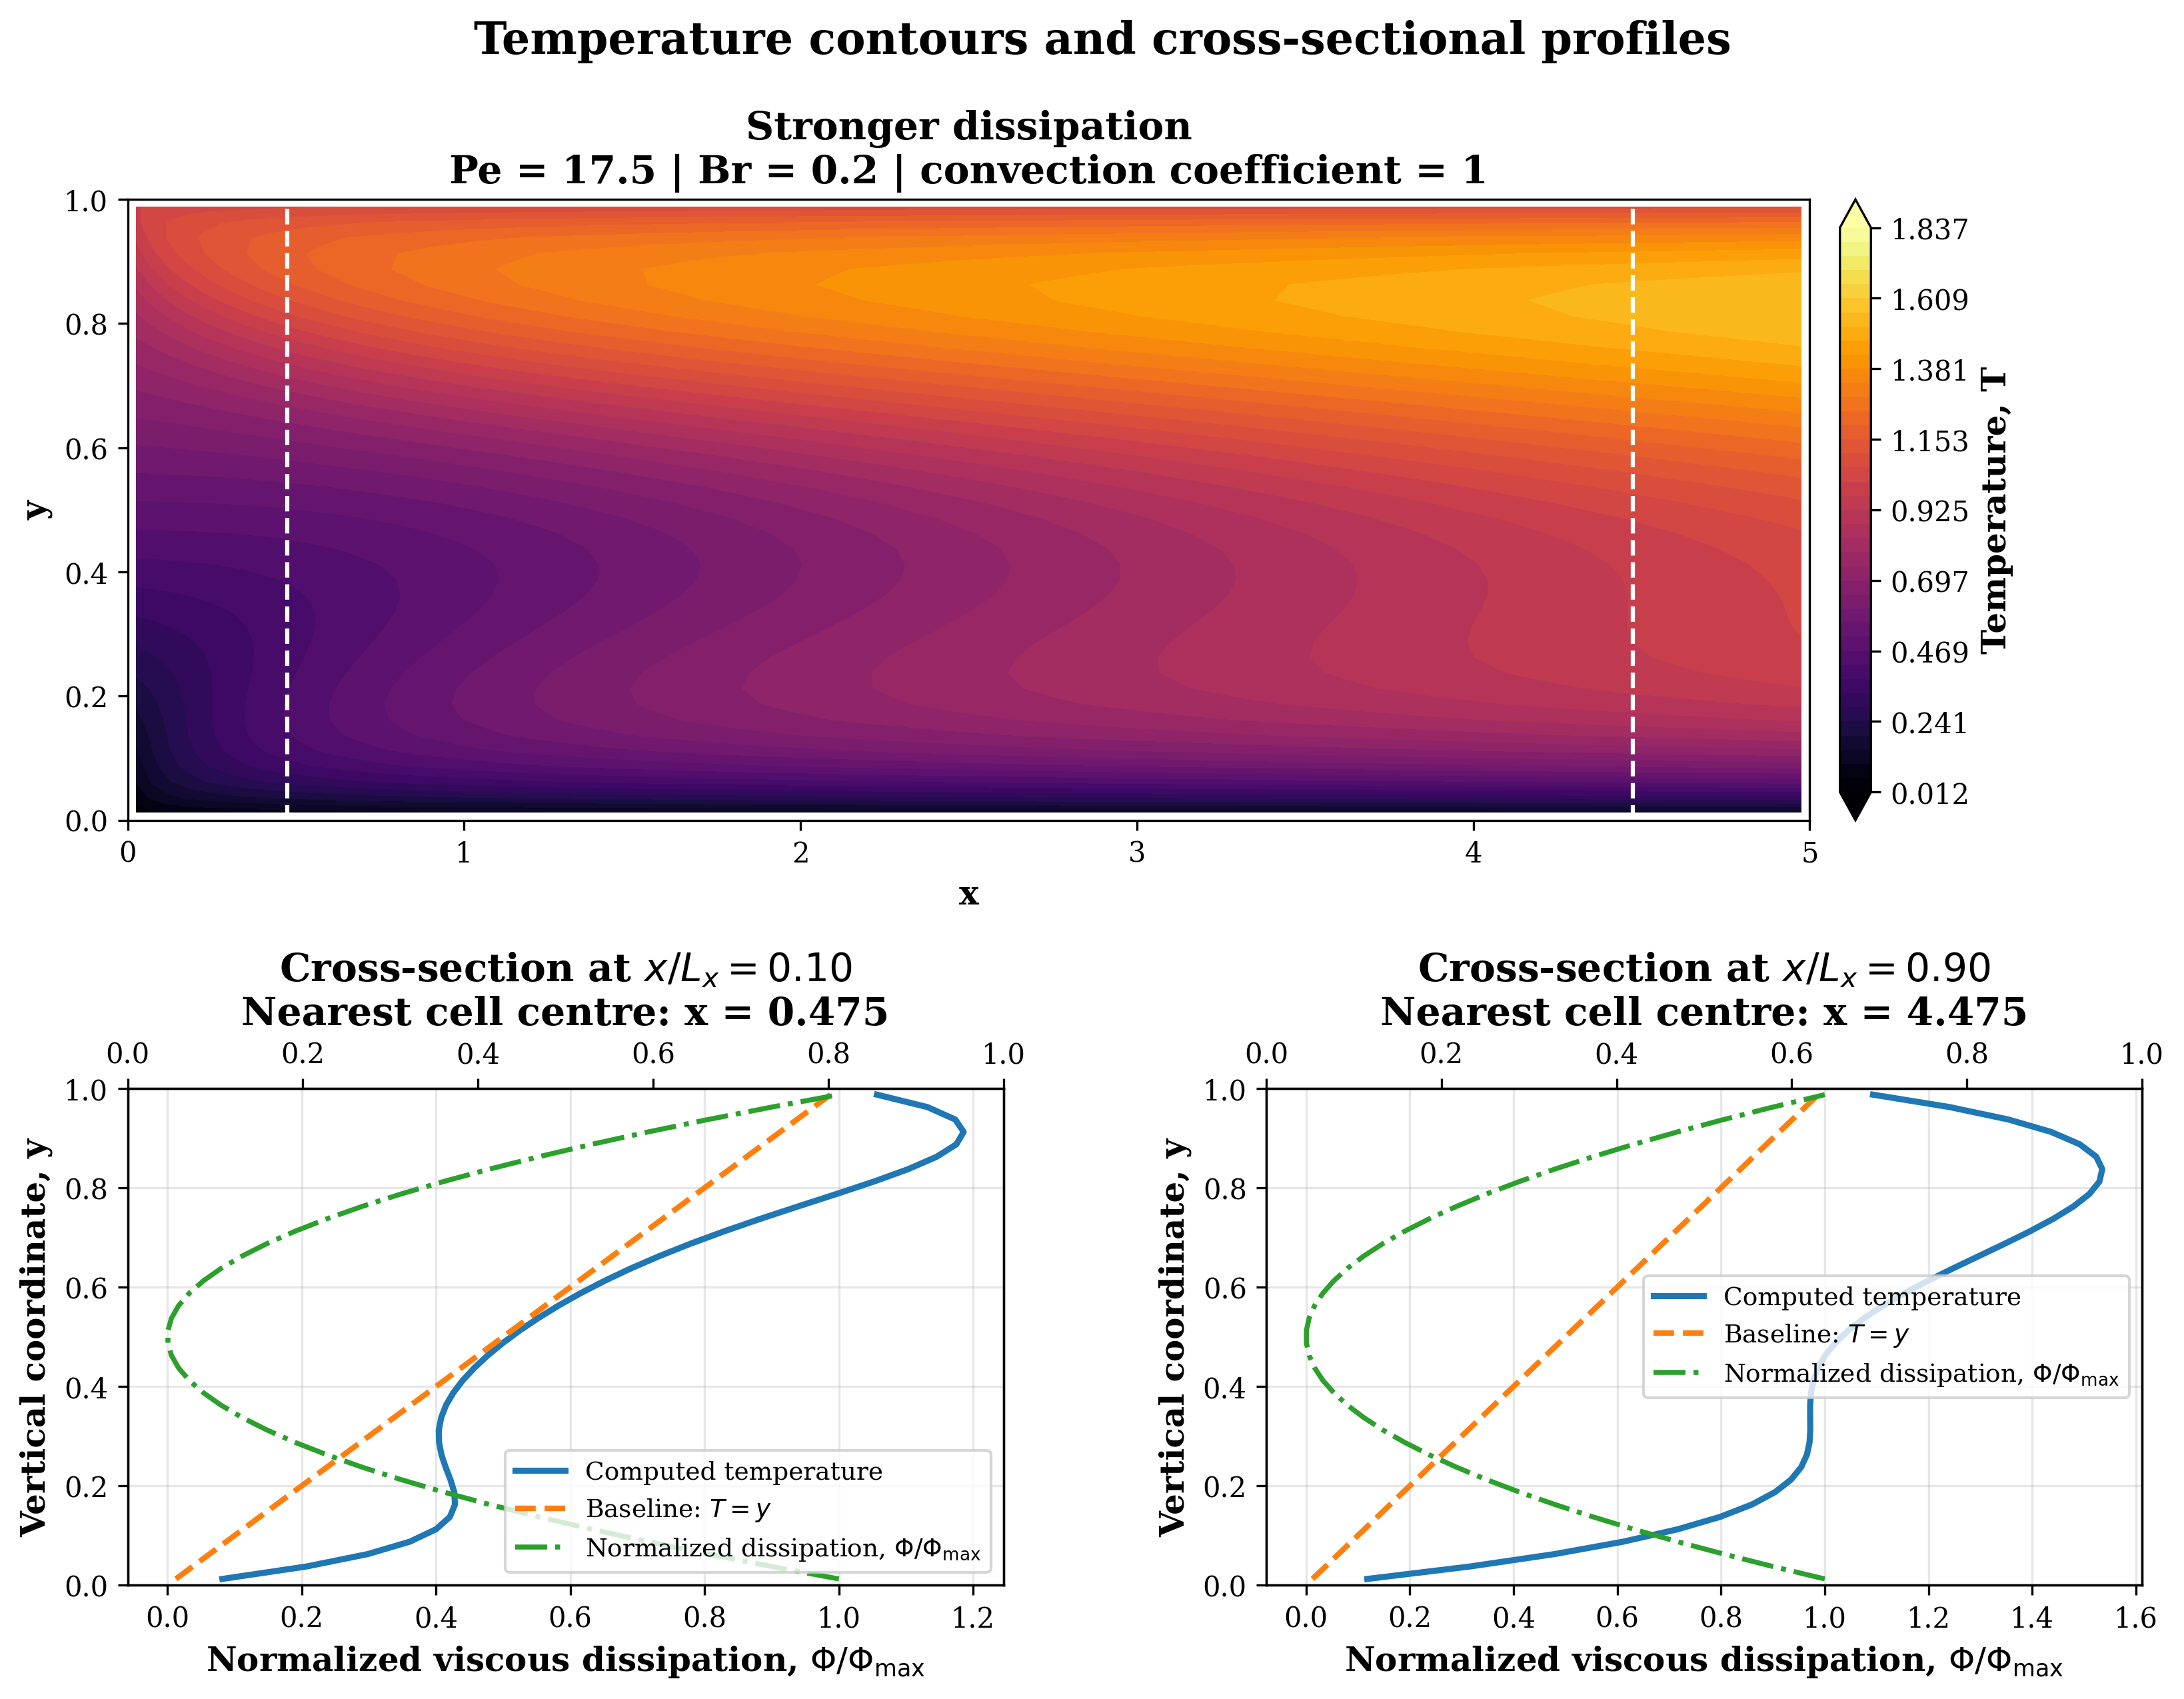
\includegraphics[width=0.88\textwidth]
    {figures/br_02_cross_sections.png}
    \caption{Temperature contours and wall-normal temperature profiles
    for $Pe=17.5$, $Br=0.2$, and $\gamma_c=1$.}
    \label{fig:cross_sections_br02}
\end{figure}

\begin{figure}[htbp]
    \centering
    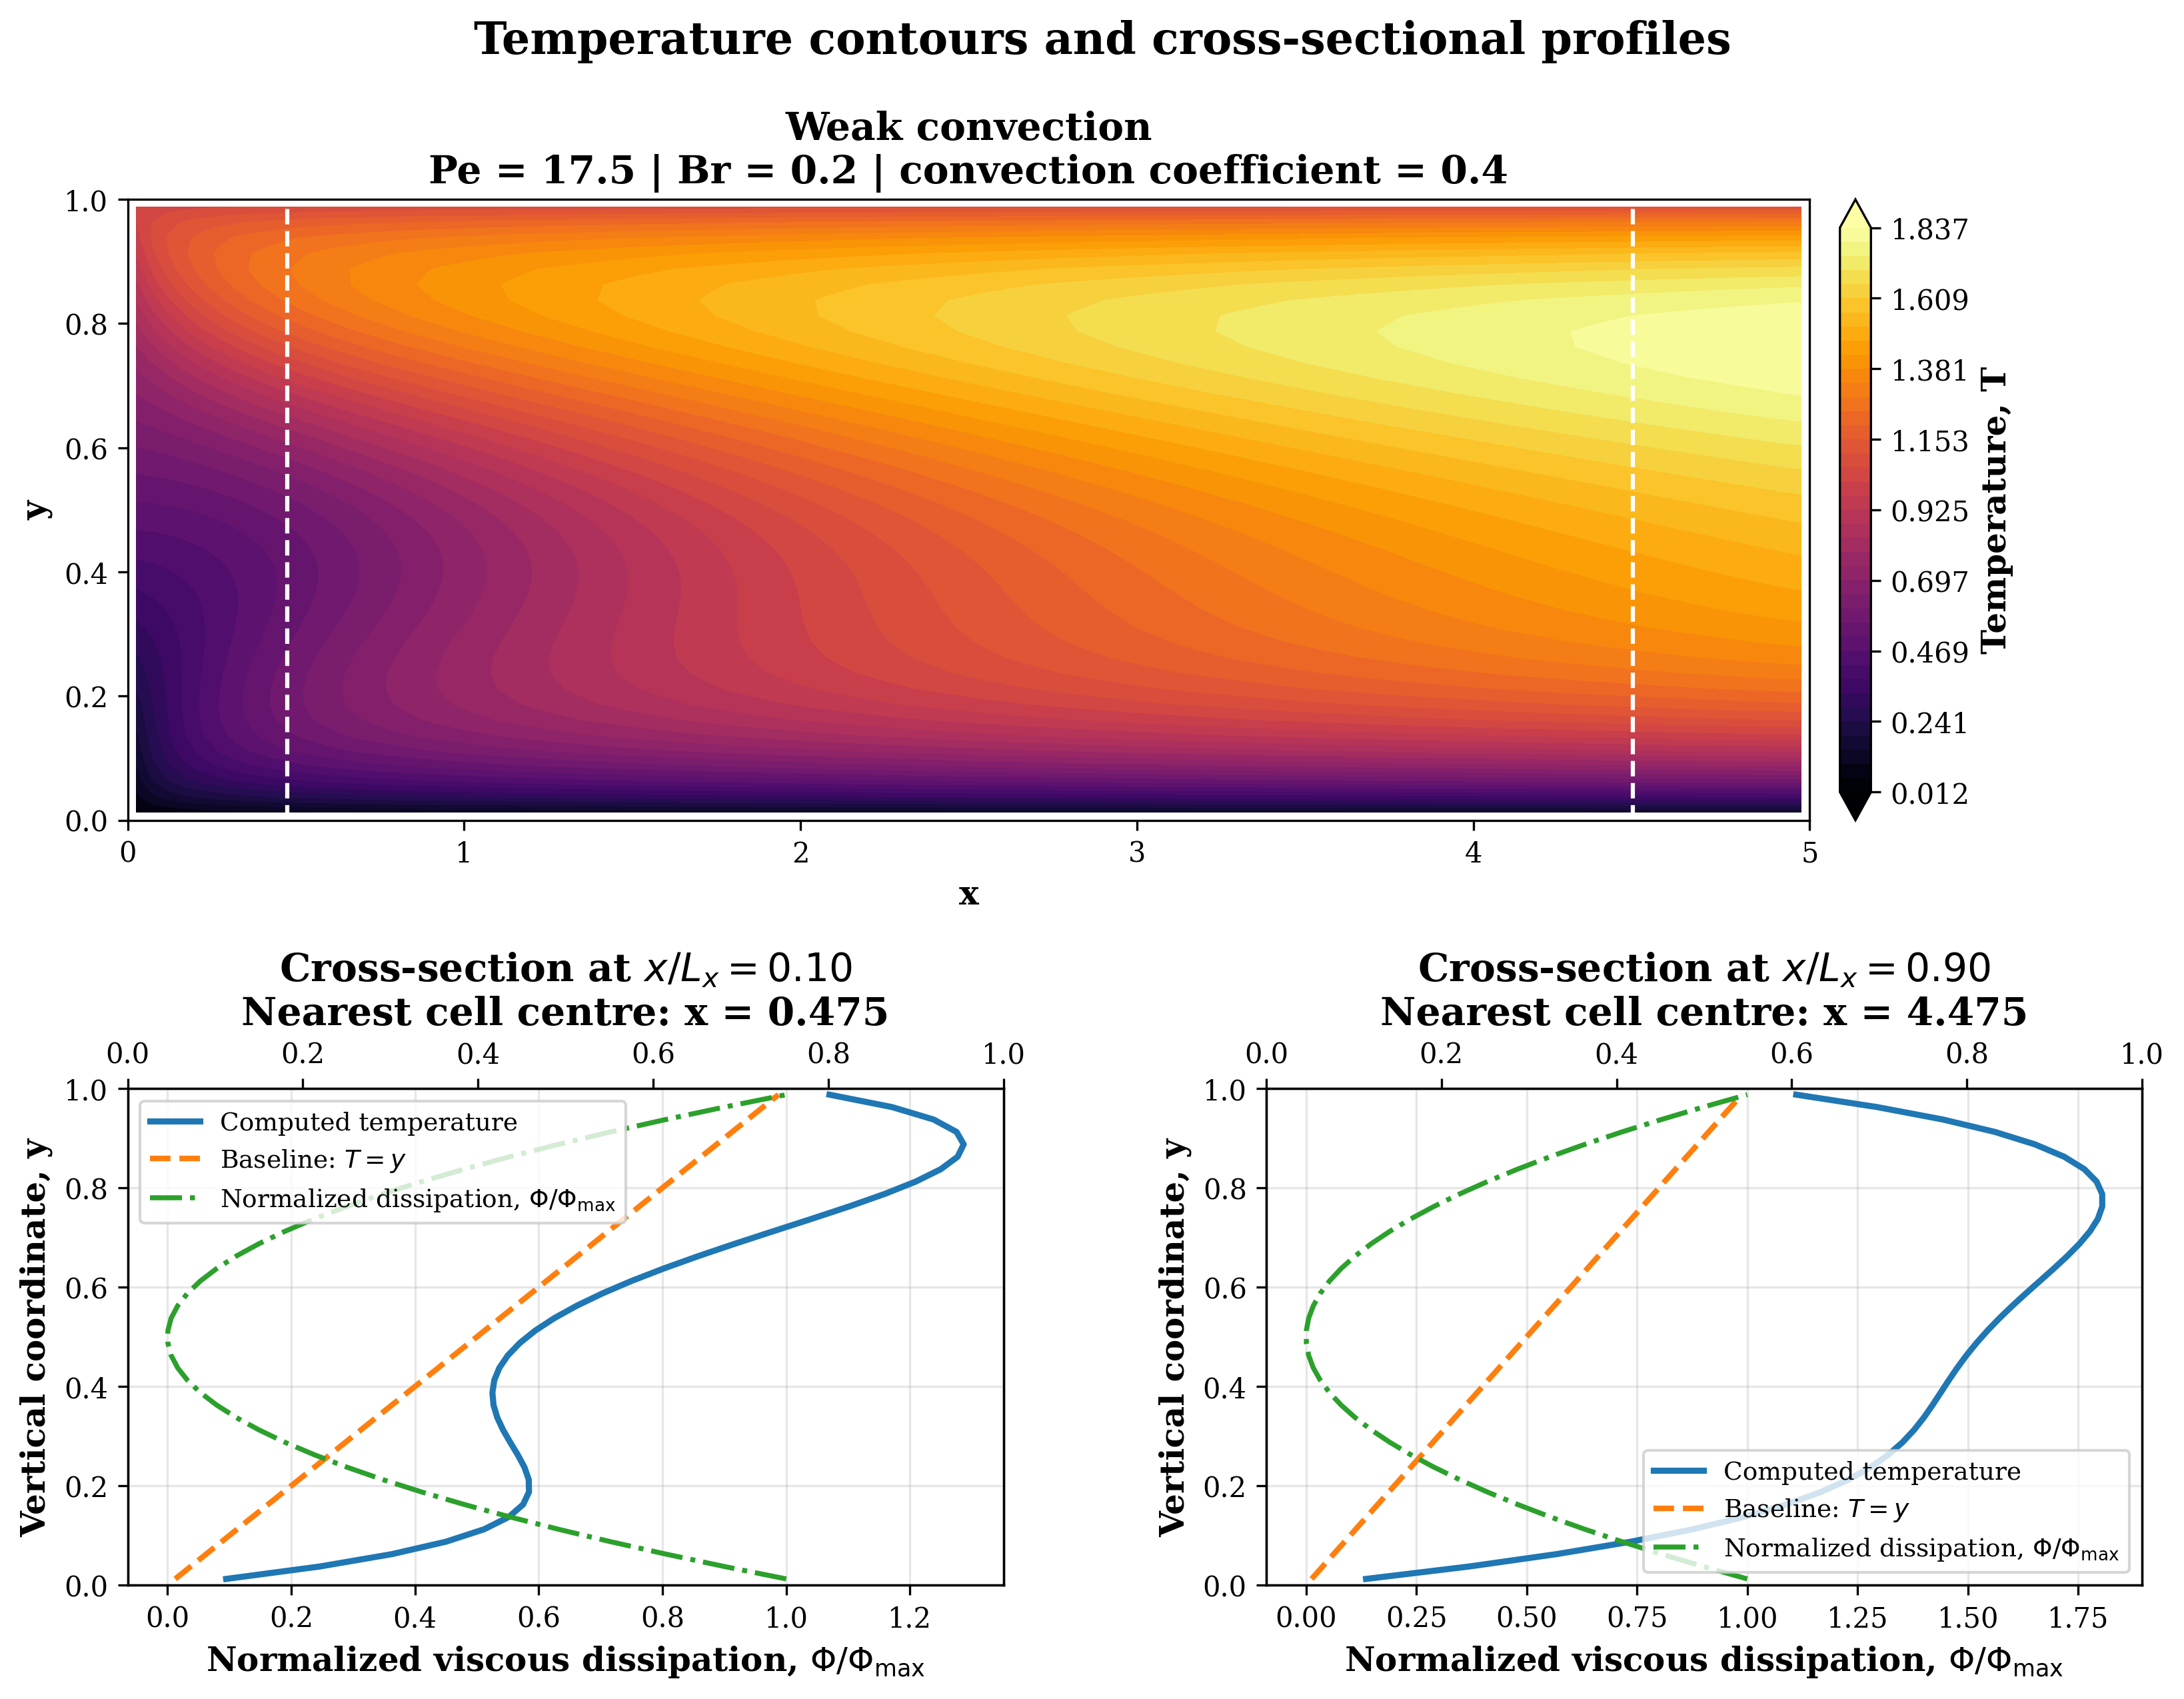
\includegraphics[width=0.88\textwidth]
    {figures/gamma_04_cross_sections.png}
    \caption{Temperature contours and wall-normal temperature profiles
    for $Pe=17.5$, $Br=0.2$, and $\gamma_c=0.4$.}
    \label{fig:cross_sections_gamma04}
\end{figure}

%------------------------------------------------
% Conclusion
%------------------------------------------------
\newpage
\section{Conclusion}

A finite-volume solver was developed to investigate the steady-state temperature distribution in a two-dimensional channel flow, accounting for convection, thermal diffusion, and viscous dissipation. The governing energy equation was discretized in space using central-difference approximations, resulting in a system of ordinary differential equations. Several time-integration methods were implemented to advance this system toward steady state, including the approximate factorization method (AFI), a sparse direct implicit method, and the explicit second- and fourth-order Runge--Kutta methods.

The numerical stability analysis showed that the explicit Runge--Kutta methods require sufficiently small time steps to maintain stability. The eigenvalue analysis provided estimates of their stability limits, which were then used to select suitable time steps for the solver comparison. The implicit methods allowed larger time steps, although their computational cost depended on the solution procedure and implementation.

The performance comparison showed that all four methods reached the prescribed residual tolerance of $10^{-12}$ on the $50\times20$ grid. Among the tested methods, the sparse direct solver achieved the shortest computation time, with a median runtime of approximately $0.14$ s. The AFI, RK2, and RK4 methods required approximately $6.28$, $8.01$, and $10.72$ s, respectively. Although RK4 required fewer iterations than RK2, its additional stages per iteration resulted in a higher total computation time. These results apply to the selected grid, time steps, convergence criterion, and implementations; they do not establish a general performance ranking for other configurations.

The temperature-field evolution illustrated the interaction between convection, thermal diffusion, and viscous dissipation during the approach to steady state. The parameter study further clarified their individual contributions. Increasing the Brinkman number strengthened viscous heating and produced larger departures from the initial linear temperature profile. Increasing the convection coefficient enhanced the downstream transport of the inlet temperature distribution, whereas reducing it allowed thermal diffusion and viscous dissipation to have a greater influence. In the Peclet-number study, the ratio $Br/Pe$ was kept constant so that the viscous-dissipation coefficient remained unchanged while the thermal-diffusion coefficient decreased with increasing Peclet number. The resulting temperature distributions demonstrated how the balance between these mechanisms determines the shape and magnitude of the temperature field.

Overall, the project provided a numerical framework for solving the two-dimensional energy equation and examining the effects of its governing parameters. The results also demonstrated that solver performance depends on the time-integration method, time-step selection, and computational implementation. Further work could include a more detailed grid-convergence study and comparisons of computational cost and accuracy over multiple grid resolutions. 


\end{document}